   \documentclass[11pt]{article}

  \usepackage{smoothing_paper}
\usepackage[section]{placeins}
\usepackage{tabularx,ragged2e,booktabs,caption}

\interfootnotelinepenalty=10000

%%%%%%%%%%%%%%%%%%%%%%%%%%%%%%%%chiheb commands

\newcommand{\ie}{\emph{i.e.}}
\newcommand{\eg}{\emph{e.g.}}
\newcommand{\cf}{\emph{cf.}}
\newcommand{\prob}[1]{\mathrm{P}\left(#1\right)}
\newcommand{\expt}[1]{\mathrm{E}\left[#1\right]}
\newcommand{\expth}[1]{\hat{\mathrm{E}}\left[#1\right]}



\newcommand{\rset}{\mathbb{R}}
\newcommand{\nset}{\mathbb{N}}
\newcommand{\zset}{\mathbb{Z}}



\newcommand{\PERIOD}{.}
\newcommand{\COMMA}{,}
\newcommand{\BIGSPACE}{\,\,\,\,\,\,\,}



\newcommand{\Ordo}[1]{{\mathcal{O}}\left(#1\right)}
\newcommand{\ordo}[1]{{o}\left(#1\right)}

%%%%%%%%%%%%%%%%%%%%%%%%%%%%%%%%%%%%%%%%%%%%%%%%%%%%%%%%%%%%%%%%%%%%%%%%
%%
%% DO WE RELLY NEED THE FOLLOWING??

%%  new margin
%%%%%%%%%%%%%%%%%%%%%%%%%%%%%%%%%%%%%%%%%%%
\pagestyle{plain}                                                      %%
%%%%%%%%%% EXACT 1in MARGINS %%%%%%%                                   %%
\setlength{\textwidth}{6.5in}     %%                                   %%
\setlength{\oddsidemargin}{0in}   %%   
\setlength{\evensidemargin}{0in}  %%        
\setlength{\textheight}{8.5in}    %%       
\setlength{\topmargin}{-0.2in}    %%   
\setlength{\headheight}{0in}      %%    
\setlength{\headsep}{0in}         %%                   
\setlength{\footskip}{.5in}       %%                       
%%%%%%%%%%%%%%%%%%%%%%%%%%%%%%%%%%%%                                   %%
\newcommand{\required}[1]{\section*{\hfil #1\hfil}}                    %%
\renewcommand{\refname}{\hfil References Cited\hfil}                   %%

\def\SMALLSKIP{\smallskip}
\def\MEDSKIP{\medskip}
\def\BIGSKIP{\bigskip}

%%
%%%%%%%%%%%%%%%%%%%%%%%%%%%%%%%%%%%%%%%%%%%%%%%%%%%%%%%%%%%%%%%%%%%%%

\makeatletter
\def\BState{\State\hskip-\ALG@thistlm}
\makeatother



%%%%%%%%%%%%%%%%%%%%%%%%%%%%%%%%%%%%%%%%

\title{ Smoothing  the  Payoff for  Efficient Computation of Option Pricing in
  Time-Stepping Setting} 
    \date{ }

\begin{document}
\maketitle

%\section{Scope and plan of the project}
%\input{scope_plan}

%\section{Motivation}

\section{Introduction}
\input{Introduction.tex}


\section{Problem formulation and Setting}\label{sec:General setting}
\input{Motivation}




%In the context of option pricing, we aim at approximating the option price, $E[g(\mathbf{X}(t))]$,  where $g:\mathbb{R}^d  \rightarrow \mathbb{R}$ is the payoff function  and where  the process of the asset prices $\mathbf{X} \in \mathbb{R}^d$ solves 
\begin{align*}
	\mathbf{X}(t)=\mathbf{X}(0)+ \int_{0}^{t} a(s,\mathbf{X}(s)) ds + \sum_{\ell=1}^{\ell_0} \int_{0}^{t} b^{\ell}(s,\mathbf{X}(s)) dW^{\ell}(s)
\end{align*}
Let us denote  by $\Phi: (\mathbf{z}_1,\dots,\mathbf{z}_N) \rightarrow \bar{\mathbf{X}}_T$, the mapping consisting of the time-stepping scheme, where $\{\mathbf{z}_i\}_{i=1}^N$ are independent $d$-dimensional Gaussian random vectors, and $N$ is the number of time steps. Without loss of Generality, we assume that $\Phi$ may include pre-processing transformations to reduce the effective dimension. We also assume that $d=1$ and the extension to higher dimension is trivial.

In this setting, we are interetsed in the basic problem of approximating
\begin{align}\label{eq:multivariate integral}
E[g(\mathbf{X}(T))] &\approx E[g(\bar{\mathbf{X}}_T)] \nonumber\\
&=\int_{\rset^N}g \circ \Phi(\mathbf{z})	d \mathbf{z}= \int_{-\infty}^{\infty} \dots \int_{-\infty}^{\infty} g \circ \Phi(z_1,\dots,z_N) \rho_d(\mathbf{z}) dz_1,\dots,dz_N \nonumber\\
&=I_N (g \circ \Phi) \COMMA
\end{align}
with
\begin{equation*}\label{eq: multivariate gaussian distribution}
\rho_N(\mathbf{z})=\frac{1}{(2 \pi)^{N/2}} e^{-\frac{1}{2} \mathbf{z}^T \mathbf{z}} \PERIOD
\end{equation*} 
where $\rho$ is a continuous and strictly positive probability density function on $\rset$ and $g$ is a real-valued function integrable with respect to $\rho_N$.
 
In this context, we work mainly with two possible structures of payoff function $g$. In fact, for the cases of call/put options, the payoff $g$ has a kink and  will be of the form 
\begin{align*}
g(\mathbf{x})=\max(\phi(\mathbf{x}),0).
\end{align*}
One can also encounter jumps in the payoff when working with binary digital options. In this case, $g$ is given by 
\begin{align*}
	g(\mathbf{x})=\mathbf{1}_{(\phi(\mathbf{x}) \ge 0)}.
\end{align*}
We introduce the notation $\mathbf{x}=(x_j,\mathbf{x}_{-j})$, where $\mathbf{x}_{-j}$ denotes the vector of length $d-1$ denoting all the variables other than $x_j$. Then, if we assume for some $j \in \{1,\dots,d\}$
\begin{align}
	\frac{\partial \phi}{\partial x_j}(\mathbf{x}) &>0,\: \forall \mathbf{x} \in \rset^d \: \: \textbf{(Monotonicity condition)}  \label{assump:Monotonicity condition}\\
	\underset{x \rightarrow +\infty}{\lim} \phi(\mathbf{x})&=\underset{x \rightarrow +\infty}{\lim} \phi(x_j,\mathbf{x}_{-j})=+\infty, \: \text{or} \:\: \frac{\partial^2 \phi} {\partial x_j^2}(\mathbf{x}) \: \: \textbf{(Growth condition)}  \label{assump:Growth condition} \COMMA
\end{align}
then, using Fubini's theorem,  we can rewrite \eqref{eq:multivariate integral} as
\begin{align}\label{eq:multivariate integral with smoothing}
I_N (g \circ \Phi) &= \int_{\rset^{d-1}} \left(\int_{-\infty}^\infty g \circ\Phi(z_j,\mathbf{z}_{-j}) \rho(z_j) dz_j  \right) \rho_{z-1}(\mathbf{z}_{-j}) d\mathbf{z}_{-j}\COMMA \\ \nonumber	  
&= \expt{E \left[g \circ\Phi(z_j,\mathbf{z}_{-j}) \mid z_j \right]}
\end{align}
where we evaluate the inner integral for each $\mathbf{z}_{-j}$ and which results in a smooth integrand for the outer $(N-1)$-dimensional integral. 

We note that  conditions (\eqref{assump:Monotonicity condition} and \eqref{assump:Growth condition}) imply that for each $\mathbf{z}_{-j}$, the function $\phi \circ \Phi(z_j,\mathbf{z}_{-j})$ either has a simple  root $z_j$ or is positive for all $z_j \in \rset$.

We generally do not have a closed form for the inside integral in \eqref{eq:multivariate integral with smoothing}. Therefore, the pre-integration (conditional sampling)  step should be performed numerically.
\section{Analyticity  and Smoothness Analysis}\label{sec:Analiticity Analysis}
\subsection{Haar construction of Brownian motion revisited}
\label{sec:haar-constr-brown}

For simplicity we shall assume throughout that we work on a fixed time
interval $[0,T]$ with $T = 1$.

With the Haar mother wavelet
\begin{equation}
  \label{eq:Haar-mother}
  \psi(t) \coloneqq
  \begin{cases}
    1, & 0 \le t < \half, \\
    -1, & \half \le t < 1, \\
    0, & \text{else},
  \end{cases}
\end{equation}
we construct the Haar basis of $L^2\left([0,1] \right)$ by setting
\begin{subequations}
  \label{eq:Haar-basis}
  \begin{gather}
    \label{eq:Haar-constant}
    \psi_{-1}(t) \coloneqq \indic{[0,1]}(t), \\
    \label{eq:Haar-nonconstant}
    \psi_{n,k}(t) \coloneqq 2^{n/2} \psi\left( 2^n t - k \right), \quad n \in
    \N_0, \ k = 0, \ldots, 2^n-1.
  \end{gather}
\end{subequations}
We note that $\supp \psi_{n,k} = [2^{-n}k, 2^{-n}(k+1)]$. Moreover, we define
a grid $\mathcal{D}^n \coloneqq \Set{t^n_\ell \mid \ell = 0, \ldots, 2^{n+1}}$ by
$t^n_\ell \coloneqq \f{\ell}{2^{n+1}}$. Notice that the Haar functions up to level
$n$ are piece-wise constant with points of discontinuity given by
$\mathcal{D}^n$.

Next we define the antiderivatives of the basis functions
\begin{subequations}
  \label{eq:Haar-int-basis}
  \begin{gather}
    \label{eq:Haar-int-constant}
    \Psi_{-1}(t) \coloneqq \int_0^t \psi_{-1}(s) ds, \\
    \label{eq:Haar-int-nonconstant}
    \Psi_{n,k}(t) \coloneqq \int_0^t \psi_{n,k}(s) ds.
  \end{gather}
\end{subequations}
For an i.i.d.~set of standard normal random variables (\emph{coefficients})
$Z_{-1}$, $Z_{n,k}$, $n \in \N_0$, $k = 0, \ldots, 2^n-1$, we can then define
a standard Brownian motion
\begin{equation}
  \label{eq:Brownian-motion}
  W_t \coloneqq Z_{-1} \Psi_{-1}(t) + \sum_{n=0}^\infty \sum_{k=0}^{2^n-1}
  Z_{n,k} \Psi_{n,k}(t),
\end{equation}
and the truncated version
\begin{equation}
  \label{eq:Brownian-motion-truncated}
  W_t^N \coloneqq Z_{-1} \Psi_{-1}(t) + \sum_{n=0}^N \sum_{k=0}^{2^n-1}
  Z_{n,k} \Psi_{n,k}(t).
\end{equation}
Note that $W^N$ already coincides with $W$ along the grid $\mathcal{D}^N$. We
define the corresponding increments for any function or process $F$ by
\begin{equation}
  \label{eq:increments}
  \Delta^N_\ell F \coloneqq F(t^N_{\ell+1}) - F(t^N_\ell).
\end{equation}

\subsection{Stochastic differential equations}
\label{sec:stoch-diff-equat}

For simplicity we consider a one-dimensional SDE $X$ given by
\begin{equation}
  \label{eq:SDE}
  dX_t = b(X_t) dW_t, \quad X_0 = x \in \R.
\end{equation}
We assume that $b$ is bounded and has bounded derivatives of all
orders. Recall that we want to compute
\begin{equation*}
  E\left[ g\left( X_T \right) \right]
\end{equation*}
for some function $g : \R \to \R$ which is not necessarily smooth.
We also define the solution of the Euler scheme along the grid $\mathcal{D}^N$
by $X^N_0 \coloneqq X_0 = x$ and
\begin{equation}
  \label{eq:euler}
  X^N_{\ell+1} \coloneqq X^N_\ell + b\left( X^N_{\ell} \right) \Delta^N_\ell W.
\end{equation}
For convenience, we also define $X^N_T \coloneqq X^N_{2^N}$.

Clearly, the random variable $X^N_\ell$ is a deterministic function of the
random variables $Z_{-1}$ and $Z^N \coloneqq \left(Z_{n,k} \right)_{n=0,
  \ldots, N, \ k=0, \ldots 2^n-1}$. Abusing notation, let us therefore write
\begin{equation*}
  X^N_\ell = X^N_\ell\left(Z_{-1}, Z^N \right)
\end{equation*}
for the appropriate (now deterministic) map $X^N_\ell: \R \times
\R^{2^{N+1}-1} \to \R$. We shall write $y \coloneqq z_{-1}$ and $z^N$ for the
(deterministic) arguments of the function $X^N_\ell$.

A note of caution is in order regarding convergence as $N \to \infty$: while
the sequence of random processes $X^N_\cdot$ converges to the solution
of~\eqref{eq:SDE} (under the usual assumptions on $b$), this is not true in
any sense for the deterministic functions.

Define
\begin{equation}
  \label{eq:H-function}
  H^N(z^N) \coloneqq E\left[ g\left( X^N_T\left( Z_{-1}, z^N \right) \right) \right].
\end{equation}
We claim that $H^N$ is analytic.

Let us consider a mollified version $g_\delta$ of $g$ and the corresponding
function $H^N_\delta$ (defined by replacing $g$ with $g_\delta$
in~\eqref{eq:H-function}). Tacitly assuming that we can interchange
integration and differentiation, we have
\begin{equation*}
  \f{\pa H^N_\delta(z^N)}{\pa z_{n,k}} = E\left[ g_\delta^\prime\left( X^N_T\left( Z_{-1},
    z^N \right) \right) \f{\pa X^N_T(Z_{-1}, z^N)}{\pa z_{n,k}}\right].
\end{equation*}
Multiplying and dividing by $\f{\pa X^N_T(Z_{-1}, z^N)}{\pa y}$ and replacing
the expectation by an integral w.r.t.~the standard normal density, we obtain
\begin{equation}
  \label{eq:1}
  \f{\pa H^N_\delta(z^N)}{\pa z_{n,k}} = \int_\R \f{\pa g_\delta\left( X^N_T
      (y, z^N) \right)}{\pa y} \left( \f{\pa X^N_T}{\pa y}(y, z^N)
  \right)^{-1} \f{\pa X^N_T}{\pa z_{n,k}}(y, z^N) \f{1}{\sqrt{2\pi}}
  e^{-\f{y^2}{2}} dy.
\end{equation}

If we are able to do integration by parts, then we can get rid of the
mollification and obtain smoothness of $H^N$ since we get
\begin{equation*}
  \f{\pa H^N(z^N)}{\pa z_{n,k}} = -\int_\R g\left( X^N_T
      (y, z^N) \right) \f{\pa}{\pa y} \left[ \left( \f{\pa X^N_T}{\pa y}(y, z^N)
  \right)^{-1} \f{\pa X^N_T}{\pa z_{n,k}}(y, z^N) \f{1}{\sqrt{2\pi}}
  e^{-\f{y^2}{2}}\right] dy.
\end{equation*}

We realize that there is a potential problem looming in the inverse of the
derivative w.r.t.~$y$.\footnote{Let us assume that
  $X^N_T(y,z^N) = \cos(y) + z_{n,k}$. Then~\eqref{eq:1} is generally not
  integrable.} Before we continue, let us introduce the following notation:
for sequences of random variables $F_N, G_N$ we say that
$F_N = \mathcal{O}(G_N)$ if there is a random variable $C$ with finite moments
of all orders such that for all $N$ we have $\abs{F_N} \le C \abs{G_N}$ a.s.

\begin{assumption}
  \label{ass:boundedness-derivative}
  There are positive random variables $C_p$ with finite moments of all orders
  such that
  \begin{equation*}
    \forall N \in \N,\ \forall \ell_1, \ldots, \ell_p \in \{0, \ldots, 2^N-1\}:\ \abs{\f{\pa^p
        X^N_T}{\pa X^N_{\ell_1} \cdots \pa X^N_{\ell_p}}} \le C_p \text{ a.s.}
  \end{equation*}
  In terms of the above notation, that means that $\f{\pa^p X^N_T}{\pa
    X^N_{\ell_1} \cdots \pa X^N_{\ell_p}} = \mathcal{O}(1)$.
\end{assumption}

\begin{remark}
  It is probably hard to argue that a deterministic constant $C$ may exist.
\end{remark}

Assumption~\ref{ass:boundedness-derivative} is natural, but now we need to
make a much more serious assumption, which is probably difficult to verify in
practice.

\begin{assumption}
  \label{ass:boundedness-inverse}
  For any $p \in \N$ we have that
  \begin{equation*}
    \left( \f{\pa X^N_T}{\pa y}\left( Z_{-1}, Z^N \right) \right)^{-p} = \mathcal{O}(1).
  \end{equation*}
\end{assumption}

\begin{lemma}
  \label{lem:dXdZ}
  We have
  \begin{equation*}
    \f{\pa X^N_T}{\pa z_{n,k}}(Z_{-1}, Z^N) = 2^{-n/2+1} \mathcal{O}(1)
  \end{equation*}
  in the sense that the $\mathcal{O}(1)$ term does not depend on $n$ or $k$.
\end{lemma}
\begin{proof}
  First let us note that Assumption~\ref{ass:boundedness-derivative} implies
  that $\f{\pa X^N_T}{\pa \Delta^N_\ell W} = \mathcal{O}(1)$. Indeed, we have
  \begin{equation*}
    \f{\pa X^N_T}{\pa \Delta^N_\ell W} = \f{\pa X^N_T}{\pa X^N_{\ell+1}}
    \f{\pa X^N_{\ell+1}}{\pa \Delta^N_\ell W} = \mathcal{O}(1) b(X^N_\ell) =
    \mathcal{O}(1).
  \end{equation*}
  Next we need to understand which increments $\Delta^N_\ell$ do depend on
  $Z_{n,k}$. This is the case iff $\supp \psi_{n,k}$ has a non-empty
  intersection with $]t^N_{\ell}, t^N_{\ell+1}[$. Explicitly, this means that
  \begin{equation*}
    \ell 2^{-(N-n+1)} -1 < k < (\ell+1) 2^{-(N-n+1)}.
  \end{equation*}
  If we fix $N$, $k$, $n$, this means that the derivative of $\Delta^N_\ell W$
  w.r.t.~$Z_{n,k}$ does not vanish iff
  \begin{equation*}
    2^{N-n+1} k \le \ell < 2^{N-n+1} (k+1).
  \end{equation*}
  Noting that
  \begin{equation}\label{eq:dWdZ}
    \abs{\f{\pa \Delta^N_\ell W}{\pa Z_{n,k}}} = \abs{\Delta^N_\ell \Psi_{n,k}}
    \le 2^{-(N-n/2)},
  \end{equation}
  we thus have
  \begin{equation}
    \label{eq:2}
    \f{\pa X^N_T}{\pa z_{n,k}}(Z_{-1}, Z^N) =
    \sum_{\ell=2^{N-n+1}k}^{2^{N-n+1}(k+1)-1} \f{\pa X^N_T}{\pa \Delta^N_\ell
      W} \f{\pa \Delta^N_\ell W}{\pa Z_{n,k}} = 2^{N-n+1} 2^{-(N-n/2)}
    \mathcal{O}(1) = 2^{-n/2+1} \mathcal{O}(1).\qedhere
  \end{equation}
\end{proof}

\begin{lemma}
  \label{lem:d2XdZdY}
  In the same sense as in Lemma~\ref{lem:dXdZ} we have
  \begin{equation*}
    \f{\pa^2 X^N_T}{\pa y \pa z_{n,k}}(Z_{-1}, Z^N) = 2^{-n/2+1} \mathcal{O}(1).
  \end{equation*}
\end{lemma}
\begin{proof}
  $\Delta^N_\ell W$ is a linear function in $Z_{-1}$ and $Z^N$, implying that
  all mixed derivatives $\f{\pa^2\Delta^N_\ell W}{\pa Z_{n,k} \pa Z_{-1}}$ vanish.
  From equation~\eqref{eq:2} we hence see that
  \begin{equation*}
    \f{\pa^2 X^N_T}{\pa z_{n,k} \pa y}(Z_{-1}, Z^N) =
    \sum_{\ell=2^{N-n+1}k}^{2^{N-n+1}(k+1)-1} \f{\pa^2 X^N_T}{\pa \Delta^N_\ell
      W \pa Z_{-1}} \f{\pa \Delta^N_\ell W}{\pa Z_{n,k} }.
  \end{equation*}
  Further,
  \begin{equation*}
    \f{\pa^2 X^N_T}{\pa \Delta^N_\ell W \pa Z_{-1}} = \sum_{j=0}^{2^{N+1}-1}
    \f{\pa^2 X^N_T}{\pa \Delta^N_\ell W \pa \Delta^N_j W} \f{\pa \Delta^N_j W}{\pa
      Z_{-1}}.
  \end{equation*}
  Note that
  \begin{equation}
    \label{eq:d2XdWdW}
    \f{\pa^2 X^N_T}{\pa \Delta^N_\ell W \pa \Delta^N_j W} = \f{\pa^2
      X^N_T}{\pa X^N_{\ell+1} \pa X^N_{j+1}} b(X^N_\ell) b(X^N_j) + \indic{j
      < \ell} \f{\pa X^N_T}{\pa X_\ell^N} b^\prime(X^N_\ell) \f{\pa
      X^N_\ell}{\pa X^N_{j+1}} b(X^N_j) = \mathcal{O}(1)
  \end{equation}
  by Assumption~\ref{ass:boundedness-derivative}. We also have $\f{\pa \Delta^N_j W}{\pa
    Z_{-1}} = \mathcal{O}(2^{-N})$, implying the statement of the lemma.
\end{proof}

\begin{remark}
  Lemma~\ref{lem:dXdZ} and~\ref{lem:d2XdZdY} also hold (mutatis mutandis) for
  $z_{n,k} = y$ (with $n = 0$).  
\end{remark}

\begin{proposition}
  \label{prop:first-derivatives}
  We have $\f{\pa H^N(z^N)}{\pa z_{n,k}} = \mathcal{O}(2^{-n/2})$ in the sense
  that the constant in front of $2^{-n/2}$ does not depend on $n$ or $k$.
\end{proposition}
\begin{proof}
  We have
  \begin{align*}
    \f{\pa H^N(z^N)}{\pa z_{n,k}} &= -\int_\R g\left( X^N_T
      (y, z^N) \right) \f{\pa}{\pa y} \left[ \left( \f{\pa X^N_T}{\pa y}(y, z^N)
  \right)^{-1} \f{\pa X^N_T}{\pa z_{n,k}}(y, z^N)  \f{1}{\sqrt{2\pi}}
                                    e^{-\f{y^2}{2}} \right] dy\\
    &= -\int_\R g\left( X^N_T(y, z^N) \right) \Biggl[- \left( \f{\pa
      X^N_T}{\pa y}(y, z^N) \right)^{-2} \f{\pa^2 X^N_T}{\pa y^2}(y, z^N)
      \f{\pa X^N_T}{\pa z_{n,k}}(y, z^N) +\\
    &\quad+ \left( \f{\pa X^N_T}{\pa y}(y, z^N) \right)^{-1} \f{\pa^2
      X^N_T}{\pa z_{n,k} \pa y}(y, z^N) - y \left( \f{\pa X^N_T}{\pa y}(y, z^N)
  \right)^{-1} \f{\pa X^N_T}{\pa z_{n,k}}(y, z^N) \Biggr] \f{1}{\sqrt{2\pi}}
                                    e^{-\f{y^2}{2}}dy.
  \end{align*}
  Notice that when $F^N(Z_{-1}, Z^N) = \mathcal{O}(c)$ for some deterministic
  constant $c$, then this property is retained when integrating out one of the
  random variables, i.e., we still have
  \begin{equation*}
    \int_\R F^N(y, Z^N) \f{1}{\sqrt{2\pi}} e^{-\f{y^2}{2}}dy = \mathcal{O}(c).
  \end{equation*}
  Hence, Lemma~\ref{lem:dXdZ} and Lemma~\ref{lem:d2XdZdY} together with
  Assumption~\ref{ass:boundedness-inverse} (for $p=2$) imply that
  \begin{equation*}
    \f{\pa H^N(z^N)}{\pa z_{n,k}} = \mathcal{O}(2^{-n/2})
  \end{equation*}
  with constants independent of $n$ and $k$.
\end{proof}

For the general case we need
\begin{lemma}
  \label{lem:d2XdZ2}
  For any $p \in \N$ and indices $n_1, \ldots, n_p$ and $k_1, \ldots, k_p$
  (satisfying $0 \le k_j < 2^{n_j}$) we have (with constants independent from
  $n_j, k_j$)
  \begin{equation*}
    \f{\pa^p X^N_T}{\pa z_{n_1,k_1} \cdots \pa z_{n_p,k_p}} (Z_1, Z^N) =
    \mathcal{O}\left( 2^{-\sum_{j=1}^p n_j/2} \right).
  \end{equation*}
  The result also holds (mutatis mutandis) if one or several $z_{n_j,k_j}$ are
  replaced by $y = z_{-1}$ (with $n_j$ set to $0$).
\end{lemma}
\begin{proof}
  We start noting that each $\Delta^N_\ell W$ is a linear function of
  $(Z_{-1},Z^N)$ implying that all higher derivatives of $\Delta^N_\ell W$
  w.r.t.~$(Z_{-1},Z^N)$ vanish. Hence,
  \begin{equation*}
    \f{\pa^p X^N_T}{\pa Z_{n_1,k_1} \cdots \pa Z_{n_p,k_p}} = \sum_{\ell_1 =
      2^{N-n_1+1} k_1}^{2^{N-n_1+1}(k_1+1) - 1} \cdots \sum_{\ell_p =
      2^{N-n_p+1} k_p}^{2^{N-n_p+1}(k_p+1) - 1} \f{\pa^p X^N_T}{\pa
      \Delta^N_{\ell_1} \cdots \pa \Delta^N_{\ell_p} W} \f{\pa
      \Delta^N_{\ell_1} W}{\pa Z_{n_1,k_1}} \cdots \f{\pa
      \Delta^N_{\ell_p}W}{\pa Z_{n_p,k_p}}.
  \end{equation*}
  By a similar argument as in~\eqref{eq:d2XdWdW} we see that
  \begin{equation*}
    \f{\pa^p X^N_T}{\pa \Delta^N_{\ell_1} \cdots \pa \Delta^N_{\ell_p} W} = \mathcal{O}(1).
  \end{equation*}
  By~\eqref{eq:dWdZ} we see that each summand in the above sum is of order
  $\prod_{j=1}^p 2^{-(N-n_j/2)}$. The number of summands in total is
  $\prod_{j=1}^p 2^{N-n_j+1}$. Therefore, we obtain the desired result. 
\end{proof}

\begin{theorem}
  \label{thr:smoothness}
  For any $p \in \N$ and indices $n_1, \ldots, n_p$ and $k_1, \ldots, k_p$
  (satisfying $0 \le k_j < 2^{n_j}$) we have (with constants independent from
  $n_j, k_j$)
  \begin{equation*}
    \f{\pa^p H^N}{\pa z_{n_1,k_1} \cdots \pa z_{n_p,k_p}}(Z^N) = 
    \mathcal{O}\left( 2^{-\sum_{j=1}^p n_j/2} \right).
  \end{equation*}
  The result also holds (mutatis mutandis) if one or several $z_{n_j,k_j}$ are
  replaced by $y = z_{-1}$ (with $n_j$ set to $0$). In particular, $H^N$ is a
  smooth function.
\end{theorem}

\begin{remark}
  \label{rem:analyticity}
  We actually expect that $H^N$ is analytic, but a formal proof seems
  difficult. In particular, note that our proof below relies on successively
  applying the above trick for enabling integration by parts: divide by
  $\f{\pa X^N_T}{\pa y}$ and then integrate by parts. This means that the
  number of terms (denoted by $\blacksquare$ below) increases fast as $p$
  increases by the product rule of differentiation. Hence, the constant in
  fron of the $\mathcal{O}\left( 2^{-\sum_{j=1}^p n_j/2} \right)$ term will
  depend on $p$ and increase in $p$. In that sense,
  Theorem~\ref{thr:smoothness} needs to be understood as an assertion about
  the anisotropy in the variables $z_{n,k}$ rather than a statement about the
  behaviour of higher and higher derivatives of $H^N$. In fact, one can see
  that in our proof the number of summands increases as $p!$ in
  $p$. Therefore, the statement of the theorem does not already imply
  analyticity. Of course, this problem is an artifact of our construction, and
  there is no reason to assume such a behaviour in general.
\end{remark}

\begin{proof}[Sketch of a proof of Theorem~\ref{thr:smoothness}]
  We apply integration by parts $p$ times as in the proof of
  Proposition~\ref{prop:first-derivatives}, which shows that we can again
  replace the mollified payoff function $g_\delta$ by the true, non-smooth one
  $g$. Moreover, from the procedure we obtain a formula of the form
  \begin{equation*}
    \f{\pa^p H^N}{\pa z_{n_1,k_1} \cdots \pa z_{n_p,k_p}} (z^N) = \int_{\R}
    g\left( X^N_T(y, z^N) \right) \blacksquare \f{1}{\sqrt{2\pi}} e^{-\f{y^2}{2}} dy,
  \end{equation*}
  where $\blacksquare$ represents a long sum of products of various
  terms. However, it is quite easy to notice the following structure: ignoring
  derivatives w.r.t.~$y$, each summand contains all derivatives
  w.r.t.~$z_{n_1,k_1}, \ldots, z_{n_p,k_p}$ exactly once. (Generally speaking,
  each summand will be a product of derivatives of $X^N_T$ w.r.t.~some
  $z_{n_j,k_j}$s, possibly with other terms such as polynomials in $y$ and
  derivatives w.r.t.~$y$ included.) As all other terms are assumed to be of
  order $\mathcal{O}(1)$ by Assumptions~\ref{ass:boundedness-derivative}
  and~\ref{ass:boundedness-inverse}, this implies the claimed result by
  Lemma~\ref{lem:d2XdZ2}. 
\end{proof}

\section{Details of our hierarchical method}\label{sec:Details of our approach}
In the following, we describe our approach which basically can be seen as a two stage method. In the first step, we use root finding procedure to get the inner integral  in \eqref{eq:multivariate integral with smoothing}, then in a second stage we employ adaptive quadraure, multi-index stochastic collocation (MISC), to compute the obtained smooth integrand.

\subsection{The one dimensional case}
For illustration purposes, let us focus on the one dimensional case, where under the risk-neutral measure, the undelying asset follows the geometric Brownian motion (GBM)
\begin{align}\label{eq:GBM_asset_price_dynamics}
dX_t= r X_t dt+\sigma X_t dB_t \COMMA 
\end{align}
		where $r$ is the risk-free rate, $\sigma$ is the volatility and $B_t$ is the standard Brownian motion. The analytical solution to  \eqref{eq:GBM_asset_price_dynamics} is 
\begin{align*}
	X_t=  X_0 \exp(( r-\sigma^2) t+\sigma B_t) \PERIOD
\end{align*}
The Brownian motion $B_t$ can be constructed either sequentially using a standard random walk construction or hierarchically using Brownian bridge (Bb) construction. To make an effective use of MISC, which profits from  anisotropy, we use the Bb construction since it produces  dimensions with different importance for MISC (creates anisotropy), contrary to random walk procedure for which all the dimension of the stochastic space have equal importance (isotropic). We explain the Bb construction in Section \ref{sec:Brwonian bridge construction}.

Let us denote by $\psi: (z_1,\dots,z_N) \rightarrow (B_1,\dots,B_N)$ the mapping of Bb construction and by $\Phi: (B_1,\dots,B_N) \rightarrow \bar{X}_T$, the mapping consisting of the time-stepping scheme. Then, we can express the option price as
\begin{align}\label{eq: option price as integral}
\expt{g(X(T))}&\approx E[g(\bar{\mathbf{X}}_T)] \nonumber\\
&=\expt{g\left(\Phi \circ \psi \right) (z_1,\dots,z_N)} \nonumber\\
&=\int_{-\infty}^{\infty} \dots \int_{-\infty}^{\infty} G(z_1,\dots,z_N)  \rho_N(\mathbf{z}) dz_1,\dots,dz_N \nonumber\\
&= I_N (G) \COMMA
\end{align}
where $G=g \circ \Phi \circ \psi$ and
\begin{equation*}\label{eq: multivariate gaussian distribution}
\rho_N(\mathbf{z})=\frac{1}{(2 \pi)^{N/2}} e^{-\frac{1}{2} \mathbf{z}^T \mathbf{z}} \PERIOD
\end{equation*}
Now, we can easily apply the procedure of pre-integration  of section \ref{sec:General setting}, where we can assume that the payoff function $g$ can be either the  maximum or indicator function and $\phi=\Phi \circ \psi$. The remaining ingredient is to determine with respect to which variable $z_j$ we will integrate.

Claiming that pre-integrating with respect to $z_1$ is the optimal option then from \eqref{eq: option price as integral}, we have
\begin{align}\label{eq: pre_integration_step_wrt_y1}
E[g(\bar{\mathbf{X}}_T)]&=\int_{-\infty}^{\infty} \dots \int_{-\infty}^{\infty} G(z_1,\dots,z_N) \rho_N(\mathbf{z}) dz_1,\dots,dz_N \nonumber\\ 
&=\int_{\rset^{N-1}} \left(\int_{-\infty}^\infty G(z_1,\mathbf{z}_{-1}) \rho(z_1) dz_1  \right) \rho_{N-1}(\mathbf{z}_{-1}) d\mathbf{z}_{-1}\nonumber\\	
&=\int_{\rset^{N-1}} h(\mathbf{z}_{-1}) \rho_{N-1}(\mathbf{z}_{-1}) d\mathbf{z}_{-1}\COMMA \\ \nonumber
	&=\expt{h(\mathbf{z}_{-1})}
\end{align}
where $h(\mathbf{z}_{-1})=\int_{-\infty}^\infty G(z_1,\mathbf{z}_{-1}) \rho(z_1) dz_1=  E\left[ G\left(z_1, \ldots, z_N \right)  \mid z_1\right] $.

Since $g$ can have a kink  or jump. Computing $h(\mathbf{z}_{-1})$ in the pre-integration step should be carried carefully to not deteriorate the smoothness of $h$. This can be done by applying a root finding procedure and then computing the uni-variate integral by summing the terms coming from integrating in each region where $g$ is smooth. In Sections (\ref{sec: Root Finding},\ref{sec:Description of the Domain Decomposition and Suitable Transformation}), we explain those points.

Once we perform stage $1$ procedure,  we use  multi-index stochastic collocation (MISC) procedure, suggested in \cite{haji2016multi}, to compute the expectation $\expt{h(\mathbf{z}_{-1})}$ . We describe the general strategy for the multi-index construction in Section \ref{sec:Details of the MISC}. 

If we denote by $\mathcal{E}_{\text{tot}}$ the total error of approximating the  expectation in \eqref{eq: option price as integral} using the MISC estimator, $Q_N$, then we have a natural error decomposition
\begin{align}\label{eq:total_error}
\mathcal{E}_{\text{tot}} & \le \abs{C_{\text{RB}}- I_{N}(G)}+\abs{I_{N}(G)-Q_{N}}\nonumber\\
  & \le \mathcal{E}_B(N)+ \mathcal{E}_Q(\text{TOL}_{\text{MISC}},N),
\end{align}
where  $\mathcal{E}_Q$ is the quadrature error, $\mathcal{E}_B$  is the bias, and $I_{N}(G)$ is the biased price computed with $N$ time steps as given by \eqref{eq: option price as integral}.

\subsection{Extension to the high dimensional case}
In the high dimensional case, we denote by $(z_1^{(i)},\dots,z_N^{(i)})$ the $N$ Gaussian independent rdvs that will be used to construct the path of the $i$-th asset $\bar{X}^{(i)}$, where $1 \le i \le d$ ($d$ denotes the number of underlyings considered in the basket). We keep the  same notations by denoting  $\psi: (z_1^{(i)},\dots,z_N^{(i)}) \rightarrow (B_1,\dots,B_N)$ the mapping of Bb construction and by $\Phi: (B^{(i)}_1,\dots,B^{(i)}_N) \rightarrow \bar{X}^{(i)}_T$, the mapping consisting of the time-stepping scheme. Then, we can express the option price as
\begin{align}\label{eq: option price as integral_basket}
	\expt{g(\mathbf{X}(T))}&\approx	\expt{g\left(\Phi \circ \psi \right) (z_1^{(1)}, \dots, z_N^{(1)}, \dots, z_1^{(d)},\dots,z^{(d)}_N)} \nonumber\\
	&=\int_{\rset^{d \times N}} G(z_1^{(1)}, \dots, z_N^{(1)}, \dots, z_1^{(d)},\dots,z^{(d)}_N)) \rho_{d \times N}(\mathbf{z}) dz_1^{(1)} \dots dz_N^{(1)} \dots z_1^{(d)} \dots dz^{(d)}_N \COMMA
\end{align}
where $G=g \circ \Phi \circ \psi$ and
\begin{equation*}
\rho_{d \times N}(\mathbf{z})=\frac{1}{(2 \pi)^{{d \times N}/2}} e^{-\frac{1}{2} \mathbf{z}^T \mathbf{z}} \PERIOD
\end{equation*}
Now,  performing the  pre-integrating step with respect to the coarse rdvs $(z_1^{(1)},\dots, z_1^{(d)} )$, results in
\begin{small}
\begin{align}\label{eq: pre_integration_step_wrt_y1_basket}
	\expt{g(\mathbf{X}(T))}&=\int_{\rset^{d \times N}} G(z_1^{(1)}, \dots, z_N^{(1)}, \dots, z_1^{(d)},\dots,z^{(d)}_N)) \rho_{d \times N}(\mathbf{z}) dz_1^{(1)} \dots dz_N^{(1)} \dots z_1^{(d)} \dots dz^{(d)}_N \nonumber\\ 
	&=\int_{\rset^{d \times (N-1)}} \left(\int_{\rset^d} G(z^{(1)}_1,\mathbf{z}^{(1)}_{-1},\dots,z^{(d)}_1,\mathbf{z}^{(d)}_{-1} ) \rho_d(z_1^{(1)},\dots,z_1^{(d)}) dz_1^{(1)}\dots dz_1^{(d)}  \right) \rho_{d \times(N-1)}(\mathbf{z}_{-1}^{(1)},\dots,\mathbf{z}_{-1}^{(d)}) d\mathbf{z}_{-1}^{(1)}\dots d\mathbf{z}_{-1}^{(d)}\nonumber\\	
	&=\int_{\rset^{d\times (N-1)}} h(\mathbf{z}^{(1)}_{-1},\dots,\mathbf{z}^{(d)}_{-1} ) \rho_{d\times (N-1)}(\mathbf{z}_{-1}^{(1)},\dots,\mathbf{z}_{-1}^{(d)}) d\mathbf{z}^{(1)}_{-1} \dots d\mathbf{z}^{(d)}_{-1}\COMMA \\ \nonumber
	&=\expt{h(\mathbf{z}^{(1)}_{-1},\dots,\mathbf{z}^{(d)}_{-1} )}
\end{align}
\end{small}
where $h(\mathbf{z}^{(1)}_{-1},\dots,\mathbf{z}^{(d)}_{-1})=\int_{\rset^d} G(z^{(1)}_1,\mathbf{z}^{(1)}_{-1},\dots,z^{(d)}_1,\mathbf{z}^{(d)}_{-1} )   \rho_d(z_1^{(1)},\dots,z_1^{(d)}) dz_1^{(1)}\dots dz_1^{(d)}$.


\subsection{The MISC method} \label{sec:Details of the MISC}

We assume that we want to approximate the expected value $\text{E}[f(Y)]$ of an analytic function $f\colon \Gamma \to \rset$ using a tensorization of quadrature formulas over $\Gamma$.

To introduce simplified notations, we start with the one-dimensional case. Let us denote by $\beta$ a non negative integer, referred to as a ``stochastic discretization level", and by $m: \nset \rightarrow \nset$  a strictly increasing function with $m(0)=0$ and $m(1)=1$, that we call  ``level-to-nodes function". At level $\beta$, we consider a set of $m(\beta)$ distinct quadrature points in $\rset$, $\mathcal{H}^{m(\beta)}=\{y^1_\beta,y^2_\beta,\dots,y_\beta^{m(\beta)}\} \subset \rset$, and a set of quadrature weights, $\boldsymbol{\omega}^{m(\beta)}=\{\omega^1_\beta,\omega^2_\beta,\dots,\omega_\beta^{m(\beta)}\}$. We also let $C^0(\rset)$ be the set of real-valued continuous functions over $\rset$. We then define the quadrature operator as
\begin{equation*}
Q^{m(\beta)}:C^0(\rset) \rightarrow \rset, \quad Q^{m(\beta)}[f]= \sum_{j=1}^{m(\beta)} f(y^j_\beta) \omega_\beta^j.
\end{equation*}
In our case, we have in \eqref{eq: pre_integration_step_wrt_y1_basket} a multi-variate integration problem with, $f:=h$, $\mathbf{Y}=(\mathbf{z}^{(1)}_{-1},\dots,\mathbf{z}^{(d)}_{-1})$,  and  $\Gamma=\rset^{d (N-1)}$, in the previous notations.  Therefore,  we define for any multi-index $\boldsymbol{\beta} \in \nset^{d (N-1)}$
$$Q^{m(\boldsymbol{\beta})}: C^0(\rset^{d (N-1)}) \rightarrow \rset,\quad  Q^{m(\boldsymbol{\beta})}= \bigotimes_{n = 1}^{d (N-1)} Q^{m(\beta_n)} \COMMA $$
where the $n$-th quadrature operator is understood to act only on the $n$-th variable of $f$. Practically, we obtain the value of $Q^{m(\boldsymbol{\beta})}[f]$  by considering the tensor grid $\mathcal{T}^{m(\boldsymbol{\beta})}= \times_{n = 1}^{d (N-1)}  \mathcal{H}^{m(\beta_n)}$ with cardinality $\#\mathcal{T}^{m(\boldsymbol{\beta})}=\prod_{n=1}^{d (N-1)} m (\beta_n)$ and computing

$$ Q^{m(\boldsymbol{\beta})}[f]= \sum_{j=1}^{\#\mathcal{T}^{m(\boldsymbol{\beta})}} f(\hat{y}_j) \bar{\omega}_j \COMMA$$
where $\hat{y}_j \in \mathcal{T}^{m(\boldsymbol{\beta})}$ and $\bar{\omega}_j$ are  products of weights of the univariate quadrature rules.
\begin{remark}
	We note that the quadrature points are chosen to optimize the convergence properties of the quadrature error.  For instance, in our context, since we are dealing with Gaussian densities, using Gauss-Hermite quadrature points is the appropriate choice.
\end{remark}
A direct approximation $\expt{f[\mathbf{Y}]} \approx Q^{\boldsymbol{\beta}}[f]$ is not an appropriate option  due to the well-known ``curse of dimensionality". We use MISC, which is a hierarchical adaptive sparse grids quadrature strategy that uses  stochastic discretizations  and classic sparsification approach to obtain an effective approximation scheme for $\expt{f}$. 

For the sake of concreteness, in our setting, we are left with a $d (N-1)$-dimensional Gaussian random input, which is chosen independently, resulting in  $d (N-1)$ numerical parameters for MISC, which we use as the basis of the multi-index construction. For a multi-index $\boldsymbol{\beta} = (\beta_n)_{n=1}^{d (N-1)} \in \mathbb{N}^{d (N-1)}$, we denote  by
$Q_N^{\boldsymbol{\beta}}$,   the result of approximating \eqref{eq: pre_integration_step_wrt_y1_basket} with a number of quadrature points  in the $i$-th dimension equal to  $m(\beta_i)$. We further define the set of
differences $\Delta Q_N^{\boldsymbol{\beta}}$ as follows: for a single index $1 \le i \le d (N-1)$,
let
\begin{equation*}
\Delta_i Q_N^{\boldsymbol{\beta}} = \left\{ 
\aligned 
 Q_N^{\boldsymbol{\beta}} &- Q_N^{\boldsymbol{\beta}'}  \text{, with } \boldsymbol{\beta}' =\boldsymbol{\beta} - e_i, \text{ if } \boldsymbol{\beta}_i>0 \\
 Q_N^{\boldsymbol{\beta}} &, \quad  \text{ otherwise}
\endaligned
\right.
\end{equation*}
where $e_i$ denotes the $i$th $d (N-1)$-dimensional unit vector. Then, $\Delta
Q_N^{\boldsymbol{\beta}}$ is defined as
\begin{equation*}
\Delta Q_N^{\boldsymbol{\beta}} = \left( \prod_{i=1}^{d (N-1)} \Delta_i \right) Q_N^{\boldsymbol{\beta}}.
\end{equation*}
Given the definition of $I^{N}(G)$ by \eqref{eq: pre_integration_step_wrt_y1_basket}, we have the telescoping property
\begin{equation*}
I^{N}(G)=Q_N^\infty = \sum_{\beta_1=0}^\infty \cdots \sum_{\beta_{d (N-1)} = 0}^\infty \Delta
Q_N^{(\beta_1, \ldots, \beta_{d (N-1)})} = \sum_{\boldsymbol{\beta} \in \mathbb{N}^{d (N-1)}} \Delta Q_N^{\boldsymbol{\beta}}.
\end{equation*}
The MISC estimator used for approximating \eqref{eq: pre_integration_step_wrt_y1_basket}, and using a set of multi-indices $\mathcal{I}\subset \nset^{d (N-1)}$ is given by
\begin{equation}\label{eq:MISC_quad_estimator}
	Q_N^{\mathcal{I}} = \sum_{\boldsymbol{\beta} \in \mathcal{I}} \Delta Q_N^{\boldsymbol{\beta}}.
\end{equation}
The quadrature error in this  case  is given by
\begin{equation}\label{eq:quadrature error}
\mathcal{E}_Q(\text{TOL}_{\text{MISC}},N) =\abs{Q_N^\infty - Q_N^\mathcal{I}} \le \sum_{\ell \in \mathbb{N}^{d(N-1)} \setminus
	\mathcal{I}} \abs{\Delta Q_N^\ell}.
\end{equation}
We define the work contribution, $\Delta \mathcal{W}_{\boldsymbol{\beta}}$, to be the computational cost  required to add  $\Delta Q_N^{\boldsymbol{\beta}}$ to $Q^{\mathcal{I}}_N$, and the error contribution, $\Delta E_{\boldsymbol{\beta}}$, to be  a measure of how much the quadrature error, defined in \eqref{eq:quadrature error}, would decrease once $\Delta Q_N^{\boldsymbol{\beta}}$  has been added to  $Q^{\mathcal{I}}_N$, that is 
\begin{align}\label{eq:Work_error_contributions}
\Delta \mathcal{W}_{\boldsymbol{\beta}} &= \text{Work}[Q^{\mathcal{I} \cup \{\boldsymbol{\beta}\}}_N]-\text{Work}[Q^{\mathcal{I}}_N] \nonumber\\
\Delta E_{\boldsymbol{\beta}} &= \abs{Q^{\mathcal{I} \cup \{\boldsymbol{\beta}\}}_N-Q^{\mathcal{I}}_N}.
\end{align}
 The  construction of the optimal  $\mathcal{I}$ will be done by profit thresholding, that is, for a certain threshold value $\bar{T}$, and a profit of a hierarchical surplus defined by
 \begin{equation*}
 P_{\boldsymbol{\beta}}= \frac{\abs{\Delta E_{\boldsymbol{\beta}}}}{\Delta\mathcal{W}_{\boldsymbol{\beta}}},
 \end{equation*}
  the optimal index set  $\mathcal{I}$  for MISC  is given by 
 $\mathcal{I}=\{\boldsymbol{\beta}: P_{\boldsymbol{\beta}}	 \ge \bar{T}\}$.
 
 
\subsection{Path generation methods (PGM)}\label{sec:Path generation methods (PGM)}

In the literature of adaptive sparse grids and  QMC, several hierarchical path generation methods (PGMs) or transformation methods have been proposed to reduce the effective dimension. Among these transformations, we cite the Brownian bridge (Bb)  construction \cite{moskowitz1996smoothness,caflisch1997valuation,morokoff1998generating,larcher2003tractability}, the principal component analysis (PCA)  \cite{acworth1998comparison} and the linear transformation (LT) \cite{imai2004minimizing}, etc \dots 

Assume that one wants to compute $\expt{g(B)}$, where $B$ is a Brownian motion with index set $[0,T]$. In most applications this is can be reasonably approximated by $\expt{\tilde{g}\left(B_{\frac{T}{N}}, \dots, B_{\frac{T N}{N}}  \right)}$, where $\tilde{g}$ is a function of the set of discrete Brownian paths.

There are three classical methods for sampling from $\left(B_{\frac{T}{N}}, \dots, B_{\frac{T N}{N}}  \right)$ given a standard normal vector $Z$, namely the forward method, the Brownian bridge (Bb) construction and the principal component analysis (PCA) construction. All of these constructions may be written in the form $\left(B_{\frac{T}{N}}, \dots, B_{\frac{T N}{N}}  \right)=AZ$, where $A$ is an $N \times N$ real matrix with 

\begin{equation}\label{eq:covariance_matrix_in_time}
A A^T =\Sigma:= \left(\frac{T}{N} \min(j,k)\right)_{j,k=1}^N=\frac{T}{N} \begin{bmatrix}
	1       & 1 & 1 & \dots & 1\\
	1     & 2 & 2 & \dots & 2 \\
	1     & 2& 3 & \dots &3 \\
	\vdots    & \vdots& \vdots & \ddots &\vdots \\
	1      & 2 & 3 & \dots &N
\end{bmatrix}
\PERIOD
\end{equation}   
For instance, the matrix $A$ corresponding to the forward method is given by 
\begin{equation*}
	A^{F} = \sqrt{\frac{T}{N}}  \begin{bmatrix}
		1       & 0  & \dots & 0\\
		1     & 1  & \dots & 0 \\
		\vdots    & \vdots & \ddots &\vdots \\
		1      & 1&  \dots &1
	\end{bmatrix}
	\PERIOD
\end{equation*}  
In the case of Bb construction, details about the construction are given in Section \ref{sec:Brwonian bridge construction}, and  the corresponding matrix $A$, For $N=8$ is given by 
 \begin{equation*}
 	A^{\text{Bb}} = \sqrt{T}  \begin{bmatrix}
 		\frac{1}{8}       & 	\frac{1}{8}   & 	\frac{\sqrt{2}}{8} & 0 &\frac{2}{8}  & 0 &0 & 0\\
 	\frac{2}{8}       & 	\frac{2}{8}   & 	\sqrt{2}\frac{ 2}{8} & 0 &0 & 0 &0 & 0\\
 		\frac{3}{8}       & 	\frac{3}{8}   & 	\frac{\sqrt{2}}{8} & 0 &0 &\frac{2}{8} &0  &0 \\
 		 	\frac{4}{8}       & 	\frac{4}{8}   & 	0 & 0 &0 & 0 &0 & 0\\
 		 	\frac{5}{8}       & 	\frac{3}{8}   & 	0 & \frac{\sqrt{2}}{8} &0 &0 &\frac{2}{8} &0 \\
 		 		\frac{6}{8}       & 	\frac{2}{8}   & 	0 & \sqrt{2}\frac{ 2}{8}  &0 & 0 &0 & 0\\
 		 			\frac{7}{8}       & 	\frac{1}{8}   & 	0 & \frac{\sqrt{2}}{8} &0 &0 &0 &\frac{2}{8}  \\
 		 			1       & 0  & 	0 & 0 &0 &0 &0 &0 \\
 	
 	\end{bmatrix}
 	\PERIOD
 \end{equation*}
When doing PCA construction \cite{acworth1998comparison}, we have $A^{\text{PCA}}=VD$, where $\Sigma=V D^2V^T$ is the singular value decomposition of $\Sigma$. 
 
\subsubsection{Brownian bridge (Bb) construction}\label{sec:Brwonian bridge construction}
In our context, sampling the Brownian motion can be constructed either sequentially using a standard random walk construction or hierarchically using   other hierarchical PGM as listed above. For our purposes, to make an effective use of MISC, which profits from anisotropy, we use the Bb construction since it produces  dimensions with different importance for MISC (creates anisotropy), contrary to random walk procedure for which all the dimension of the stochastic space have equal importance (isotropic).  This pre-transformation  reduces the effective dimension dimension  of the problem and as a consquence accelerates the MISC procedure by reducing the computational cost.

Let us denote $\{t_i\}_{i=0}^{N}$ the grid of time steps, then the Bb construction \cite{glasserman2004monte} consists of the following: given a past value $B_{t_i}$ and a future value $B_{t_k}$, the value $B_{t_j}$ (with $t_i < t_j < t_k$) can be generated according to the formula:
\begin{equation}
B_{t_j}=(1-\rho) B_{t_i}+\rho B_{t_k}+ \sqrt{\rho (1-\rho)(k-i) \Delta t} z, \: z \sim \mathcal{N}(0,1) \COMMA
\end{equation}
where $\rho=\frac{j-i}{k-i}$.  In particular, if $N$ is a power of $2$, then given $B_0=0$, Bb generates the Brownian motion at times $T, T/2,T/4,3T/4,\dots$ according
\begin{align}\label{eq:BB construction}
	B_T&=\sqrt{T}z_1\nonumber\\
	B_{T/2}&= \frac{1}{2}(B_{0}+B_{T})+\sqrt{T/4}z_2= \frac{\sqrt{T}}{2} z_1+\frac{\sqrt{T}}{2} z_2\nonumber\\
	B_{T/4}&=\frac{1}{2} (B_{0}+B_{T/2})+\sqrt{T/8}z_3= \frac{\sqrt{T}}{4} z_1+\frac{\sqrt{T}}{4} z_2+\sqrt{T/8}z_3\nonumber\\
	\vdots \nonumber\\
\end{align}
where $\{z_j\}_{j=1}^{N}$ are independent standard normal variables. 

Describing construction \ref{eq:BB construction}: we  first generate the final value $B_T$, then sample $B_{T/2}$ conditional
on the values of $B_T$ and $B_0$, and proceed by progressively filling in intermediate values. Bb uses the first several coordinates of the low-discrepancy points to determine the general shape of the Brownian path, and the last few coordinates influence only the fine detail of the path. Therefore, the most important values that determine the large scale structure of Brownian motion are the first components of $\mathbf{z} = (z_1,\dots,z_N)$.  

\subsection{Richardson extrapolation}\label{sec:Richardson extrapolation}
Another transformation that we coupled with MISC is Richardson extrapolation \cite{talay1990expansion}. In fact, applying level $K_\text{R}$ (level of extrapolation) of Richardson extrapolation reduces dramatically the bias and as a consequence reduces the  number of time steps $N$ needed in the coarsest level to achieve a certain error tolerance. This means basically that Richardson extrapolation directly reduces  the total dimension of the integration problem for achieving some error tolerance.

We  recall that the Euler scheme has weak order one so that
\begin{align}\label{Euler_weak_error}
	\abs{\expt{f(\hat{X}_T^h)}-\expt{f(X_T)} }  \leq C h
\end{align}
for some constant $C$, all sufficiently small $h$ and suitably smooth $f$. It can be easily  shown that  \eqref{Euler_weak_error} can be improved to
\begin{align}\label{Euler_weak_error_strenghten}
	\expt{f(\hat{X}_T^h)}= \expt{f(X_T)} + c h +\Ordo{h^2} \COMMA
\end{align}
where $c$ depends on $f$. 

Applying \eqref{Euler_weak_error_strenghten} with discretization step $2h$, we  obtain
\begin{align*}
	\expt{f(\hat{X}_T^{2h})}= \expt{f(X_T)} + 2 c h +\Ordo{h^2} \COMMA
\end{align*}
implying
\begin{align*}
	2 \expt{f(\hat{X}_T^{2h})}- \expt{f(\hat{X}_T^{h})} =\expt{f(X_T)} + \Ordo{h^2} \COMMA
\end{align*}
For higher levels of extrapolations, we use the following: Let us denote by $h_J=h_0 2^{-J}$ the grid sizes (where $h_0$ is the coarsest grid size), by $K_\text{R}$ the level of the Richardson extrapolation, and by $I(J,K_\text{R})$ the approximation of $\expt{f((X_T)}$ by terms up to level $K_\text{R}$ (leading to a weak error of order $K_\text{R}$), then we have the following recursion 
\begin{align*}
I(J,K_\text{R})=\frac{2^{K_\text{R}}\left[I(J,K_\text{R}-1)-I(J-1,K_\text{R}-1)\right]}{2^{K_\text{R}}-1},\quad J=1,2,\dots, K_\text{R}=1,2,\dots
\end{align*}
\begin{remark}
We emphasize that through our work, we are interested in the pre-asymptotic regime (small number of time steps), and the use of Richardson extrapolation is justified by our observed experimental results in that regime (see Section \ref{sec:Weak error plots_no_change}),  which in particular, show an order one of convergence for the weak error. Although, we do not claim that the observed rates will scale well in the asymptotic regime, we observed that the pre-asymptotic regime is enough to get sufficiently accurate estimates for the option prices. 
\end{remark}

\subsection{Root Finding}\label{sec: Root Finding}
Without loss of generality, we can assume that the integration domain  can
be divided into two parts $\Omega_1$, and $\Omega_2$ such that the integrand $f$ is smooth and positive in $\Omega_1$ whereas $f(\mathbf{x}) = 0$ in $\Omega_2$. Therefore,
\begin{equation}
I f := \int_{\Omega_1} f(\mathbf{x}) d \mathbf{x}
\end{equation}
This situation may arise when the integrand is non-differentiable or noncontinuous along the boundary between $\Omega_1$ and $\Omega_2$. For these problems, kinks and jumps can efficiently be identified by a one-dimensional root finding. Then, the kinks and jumps can
be transformed to the boundary of integration domain such that they no longer deteriorate the performance of the numerical methods. In fact, we  compute the zeros of the integrand  with respect to  the last dimension. In this dimension, then, e.g., Newton's method or bisection can be used to identify the point which separates $\Omega_1$ and $\Omega_2$. In our project, we use Newton 's iteration solver.

Let us call $y$ the mapping such that: $y: \mathbf{z}_1 \rightarrow z^{\text{kink}}$, where  $z^{\text{kink}}$ is   the "location of
irregularity", \ie,  $g$ is not smooth at the point $\phi \circ \Phi \circ \Psi(z^{\text{kink}}, \mathbf{z}_{-1})$. Generally, there might be (for given $\mathbf{z}_{-1}$
\begin{itemize}
	\item no solution, i.e., the integrand in the definition of $h(\mathbf{z}_{-1})$ above
	is smooth (\textit{best case});
	\item a unique solution;
	\item multiple solutions.
\end{itemize}

Generally, we need to assume that we are in the first or second
case. Specifically, we need that
\begin{equation*}
	\mathbf{z}_{-1} \mapsto h(\mathbf{z}_{-1}) \text{ and } \mathbf{z}_{-1} \mapsto \hat{h}(\mathbf{z}_{-1})
\end{equation*}
are smooth, where $\hat{h}$ denotes the numerical approximation of $h$ based
on a grid containing $y(\mathbf{z}_{-1})$. In particular, $y$ itself should be smooth
in $\mathbf{z}_{-1}$. This would already be challenging in practice in the third
case. Moreover, in the general situation we expect the number of solutions $y$ to increase when the discretization of the SDE gets finer.

In many situations, case $2$ (which is thought to include case 1) can be
guaranteed by monotonicity (\red{I think we need to add also the growth condition}. For instance, in the case of one-dimensional SDEs
with $z_1$ representing the terminal value of the underlying Brownian motion (and $\mathbf{z}_{-1}$ representing the Brownian bridge), this can often be seen from the SDE itself. Specifically, if each increment ``$dX$'' is increasing in $z_1$, no matter the value of $X$, then the solution $X_T$ must be increasing
in $z_1$. This is easily seen to be true in examples such as the Black-Scholes model and the CIR process. (Strictly speaking, we have to distinguish between the continuous and discrete time solutions. In these examples, it does not matter.) On the other hand, it is also quite simple to construct counter examples, where monotonicity fails, for instance SDEs for which the ``volatility'' changes sign, such as a trigonometric function.\footnote{Actually, in every such case the simple remedy is to replace the volatility by its absolute value, which does not change the law of the solution. Hence, there does not seem to be a one-dimensional counter-example.}

Even in multi-dimensional settings, such monotonicity conditions can hold in specific situations. For instance, in case of a basket option in a multivariate Black Scholes framework, we can choose a linear combination $z_1$ of the terminal values of the driving Bm, such that the basket is a monotone function of $z_1$. (The coefficients of the linear combination will depend on the correlations and the weights of the basket.) However, in that case this may actually not correspond to the optimal ``rotation'' in terms of optimizing the smoothing effect.

\subsection{Description of the Domain Decomposition and Suitable Transformation}\label{sec:Description of the Domain Decomposition and Suitable Transformation}
The payoff function is not smooth due to
the nature of the option. In fact, the holder would not exercise
the option if a purchase or sale of the underlying asset would lead to a loss. As a result, the discontinuity of the payoff function carries over to the integrand. In this case, The integrand shows a kink  or even a jump with respect to a  manifold. Since some
(mixed) derivatives are not bounded at these manifolds, the smoothness requirements for the sparse grid method are clearly not fulfilled any more.

The first step consists of identifying the areas 
of discontinuity or non-differentiability. Then, we decompose the total integration domain $\Omega$ into sub-domains $\Omega_i,\: i=1,\dots,n$ such that the integrand is smooth in the interior of 
$\Omega_i$ and such that all kinks and jumps are
located along the boundary of these areas.  This procedure results in integrating several smooth functions, instead of one discontinuous function. The total integral is then given
as the sum of the separate integrals, \ie
\begin{align}
	I f := \int_{\Omega} f(\mathbf{x}) d \mathbf{x}=\sum_{i=1}^{n}	\int_{\Omega_i} f(\mathbf{x}) d \mathbf{x}
\end{align}
In this way, the fast convergence of SG can
be regained whereas the costs only increase by a constant (the number of terms in
the sum), provided the cost required for the decomposition is sufficiently small such that it can be neglected.

In general, such a decomposition is even more expensive than to integrate the function. Nevertheless, for some problem classes, the areas of discontinuity have a particular simple form, which allows to decompose the integration domain with
costs that are much smaller than the benefit which results from the decomposition.  In this work, we consider those cases.

In the literature, there two classes that have been tackled. In the first one, we have the information that the kinks are  part of the integration domain where the integrand is zero and can thus be identified by root finding as proposed in \cite{gerstner2007sparse}.

In the second class, we have the information that the discontinuities are located on hyperplanes, which allows a decomposition first into polyhedrons and then into
orthants as discussed in \cite{gerstner2008valuation}. In this work, we start by the first  class of problems.



\section{Error discussion}\label{sec:Error discussion}
\subsection{Errors in smoothing}
\label{sec:errors-smoothing}

For the analysis it is useful to assume that $\hat{h}$ is a smooth function of $(\mathbf{y}_{-1},\mathbf{z}^{(1)}_{-1},\dots,\mathbf{z}^{(d)}_{-1} )$, but in reality this is not going to be true. Specifically, if the true location $y_1^\ast$ of the non-smoothness in the system was available, we could actually guarantee $\hat{h}$ to be smooth, for instance by choosing 
\begin{equation*}
	\hat{h}(\mathbf{y}_{-1},\mathbf{z}^{(1)}_{-1},\dots,\mathbf{z}^{(d)}_{-1}  ) = \sum_{k=-K}^{K} \eta_k G\left( \zeta_k(R(\mathbf{y}_{-1},\mathbf{z}^{(1)}_{-1},\dots,\mathbf{z}^{(d)}_{-1} )),
	\mathbf{y}_{-1},\mathbf{z}^{(1)}_{-1},\dots,\mathbf{z}^{(d)}_{-1}   \right),
\end{equation*}
for points $\zeta_k \in \R$ with $\zeta_0 = y_1$ and corresponding weights
$\eta_k$.\footnote{Of course, the points $\zeta_k$ have to be chosen in a
	systematic manner depending on $y_1$.} However, in reality we have to approximate numerically $R$ by $\bar{R}$ with error
$\abs{R(\mathbf{y}_{-1},\mathbf{z}^{(1)}_{-1},\dots,\mathbf{z}^{(d)}_{-1}) - \bar{R}(\mathbf{y}_{-1},\mathbf{z}^{(1)}_{-1},\dots,\mathbf{z}^{(d)}_{-1}  )} \le \delta$. Now, the actual integrand in $(\mathbf{y}_{-1},\mathbf{z}^{(1)}_{-1},\dots,\mathbf{z}^{(d)}_{-1})$ becomes 
\begin{equation*}
	\bar{h}(\mathbf{y}_{-1},\mathbf{z}^{(1)}_{-1},\dots,\mathbf{z}^{(d)}_{-1}  ) \coloneqq \sum_{k=-K}^{K} \eta_k G\left( \zeta_k(\bar{R}(\mathbf{y}_{-1},\mathbf{z}^{(1)}_{-1},\dots,\mathbf{z}^{(d)}_{-1} )),
	\mathbf{y}_{-1},\mathbf{z}^{(1)}_{-1},\dots,\mathbf{z}^{(d)}_{-1}   \right),
\end{equation*}
which we cannot assume to be smooth anymore. On the other hand, if
$\zeta_k(y)$ is a continuous function of $R$, and $R$ and $\bar{R}$ are continuous in $(\mathbf{y}_{-1},\mathbf{z}^{(1)}_{-1},\dots,\mathbf{z}^{(d)}_{-1}  )$, then \emph{eventually} we will have
\begin{equation*}
	\norm{\hat{h} - \bar{h}}_\infty \le \tol, \quad \norm{h - \bar{h}}_\infty
	\le \tol, 
\end{equation*}
i.e., the smooth functions $h$ and $\hat{h}$ are close to the integrand $\bar{h}$. (Of course, this may depend on us choosing a good enough quadrature
$\zeta$!) 
\begin{remark}
	If the adaptive collocation used for computing the integral of $\bar{h}$
	depends on derivatives (or difference quotients) of its integrand $\bar{h}$,
	then we may also need to make sure that derivatives of $\bar{h}$ are close
	enough to derivatives of $\hat{h}$ or $h$. This may require higher order
	solution methods for determining $y$.
\end{remark}
\red{We need to check the impact of the error caused by the Newton iteration on the integration error. In the worst case, we expect that if the error in the Newton iteration is of order $O(\epsilon)$ than the integration error will be of order $\operatorname{log}(\epsilon)$. But we need to check that too.}

%\begin{remark}
%	In some important cases, $f$ may be trivial (e.g., $\equiv 0$). In these
%	cases, we may be able to make sure that $\bar{y}$ never crosses the ``location of
%	non-smoothness''. Then even $\bar{h}$ is smooth.
%\end{remark}
%
%\begin{remark}
%	We expect that the global error of our procedure will be bounded by the weak error which is in our case of order $O(\Delta t)$. In this case, the overall complexity of our procedure will be of order $O(TOL^{-1})$. We note that this rate can be improved up to $O(TOL^{-\frac{1}{2}})$ if we use Richardson extrapolation. Another way that can improve the complexity could be based on Cubature on Wiener Space (This is left for a future work). The aimed complexity rate illustrates the contribution of our procedure which outperforms  Monte Carlo forward Euler (MC-FE) and multi-level MC-FE, having complexity rates of order $O(TOL^{-3})$  and $O(TOL^{-2} log(TOL)^2)$  respectively. 
%\end{remark}




\section{Numerical experiments for Numerical smoothing with ASGQ}
In this section, we conduct our experiments for four different examples: i) single binary option under discretized GBM model, ii) single call option under discretized GBM model, iii) $2d$-basket call option under discretized GBM model and iv) $4d$-basket call option under discretized GBM model .

For each example, we estimate the weak error  (Bias) of MC, then we conduct a comparison between MC and ASGQ in terms of errors and computational time. We show tables and plots reporting  the different relative errors involved in the MC method (bias and statistical error\footnote{The statistical error estimate of MC is  $C_{\alpha} \frac{\sigma_M}{\sqrt{M}}$, where $M$ is the number of samples and $C_{\alpha}=1.96$ for $95\%$ confidence interval.}  estimates), and in ASGQ (bias and quadrature error estimates).  While fixing  a  sufficiently small error tolerance in the price estimates,  we also compare the computational time needed for both methods to meet the desired error tolerance.  We note that  in all cases the actual work (runtime) is obtained using an Intel(R) Xeon(R) CPU E$5$-$268$ architecture. 

Through our conducted numerical experiments for each parameter set, we follow these steps to achieve our reported results:
\begin{enumerate}
\item[i)] For a fixed number of time steps, $N$, we compute an accurate estimate, using a large number of samples, $M$, of the biased  MC solution. This step also provides us with an estimate of the bias error, $\mathcal{E}_B(N)$, defined by \eqref{eq:total_error}. 
\item[ii)] The estimated  biased solution is used as a reference solution  to ASGQ to compute the quadrature error, $\mathcal{E}_Q(\text{TOL}_{\text{ASGQ}},N)$, defined by \eqref{eq:quadrature error}.
\item[iii)] In order to compare with MC method, the number of samples, $M$, is chosen so that  the statistical error of the Monte Carlo  method, $\mathcal{E}_S(M)$, satisfies
\begin{align}\label{optimal_number_samples}
\mathcal{E}_S(M)= \mathcal{E}_B(N)=\frac{\mathcal{E}_{\text{tot}}}{2}\COMMA
\end{align}
where $\mathcal{E}_B(N)$ is the bias as defined in \eqref{eq:total_error} and
$\mathcal{E}_{\text{tot}}$ is the total error. 
\end{enumerate}
We show  the summary of our numerical findings in Table \ref{table:Summary of our numerical results.}, which  highlights the computational gains achieved by ASGQ over MC method to meet a certain error tolerance, which we set approximately to $1\%$. More detailed results for each case  are provided in  Sections \ref{sec:Results for the binary option example}, \ref{sec:Results for the call option example} and \ref{sec:The basket call option  under GBM  model}.

Along the numerical part below, we compare $3$ methods:
\begin{enumerate}
\item[i)] Adaptive sparse grids quadrature (ASGQ) based on construction as explained in Section \ref{sec:Details of the ASGQ}.
\item[ii)] Plain Monte Carlo where we apply standard Monte Carlo and we refer to it by "MC".
\item[iii)] Monte Carlo applied to the smoothed payoff function after numerical smoothing and we refer to it by "MC+ root finding".
\end{enumerate}
\FloatBarrier
\begin{table}[!h]
	\centering
	\begin{small}
	\begin{tabular}{l*{4}{c}r}
	\toprule[1.5pt]
		Example          & Level of Richardson extrapolation    &  Total relative error  & CPU time  $\left(\text{MC}/ \text{ASGQ} \right)$ \\
		\hline
			  Single binary option (GBM) & without  &  $2 \%$&  $ 4$ \\	
              \hline
            Single call option (GBM)  & without    &  $0.9\%$&  $22$ \\
%            & level $1$ &  $$ &  $$ \\		
				 \hline
					$2d$-Basket call option (GBM)  & without    &  $$0.9\%$$&  $21$ \\	
					\hline
					$4d$-Basket call option (GBM)  & without    &  $$0.8\%$$&  $27$ \\	
		\bottomrule[1.25pt]
	\end{tabular}
\end{small}
	\caption{Summary of relative errors and computational gains, achieved by the different methods. In this table, we highlight the computational gains achieved by ASGQ over MC method to meet a certain error tolerance. We provide details about the way we compute these gains for each case in the following sections.}
	\label{table:Summary of our numerical results.}
\end{table}
\FloatBarrier

\subsection{Options under the discretized one dimensional GBM model}\label{sec:The discretized 1D Black-Scholes}
The first two  examples that we will  test are  the single binary and  call options under GBM model where the process $X$ is the discretized one dimensional GBM model and the payoff function $g$ is the indicator or maximum function as given by \eqref{eq:binary_option} and \eqref{eq:call_option} respectively. Precisely, we are interested in the  one dimensional lognormal example where the dynamics of the stock are given by
\begin{align}\label{lognormal_dynamics}
	dX_t=\sigma X_t dW_t,
\end{align}
where $\{W_t, 0 \leq t \leq T\} $ is a standard one-dimensional Brownian motion. In the discrete case, the numerical approximation of $X(T)$, using $N$ time steps ($\Delta t=\frac{T}{N}$), satisfies
\begin{align}
	\bar{X}_T&=\Psi(\Delta t, z_1, \Delta B_0,\dots,\Delta B_{N-1}), \\ \nonumber
	&=\Psi(\Delta t, \Phi(z_1,\dots,z_N))\COMMA
\end{align}
wehre $(z_1,\dots,z_N)$ are standard Gaussian random variables, for some path function $\Psi$ and Brownian bridge map $\Phi$. As explained in Sections \ref{sec:Discrete time, practical motivation} and \ref{sec:Details of our approach}, the first step of our approach is determining the location of irregularity (kink). In the following, we want to compare different ways for identifying the location of the kink for this model.
\subsubsection{Determining the kink location}\label{sec:Determining the kink location}
\subsubsection*{Exact location of the kink for the continuous problem}
Let us denote $y^{\ast}$ an invertible function that satisfies 
\begin{align}\label{eq: kink_point_problem}
	X(T;y^{\ast}(x),B)=x.
\end{align}
We can easily prove that the expression of $y^{\ast}$ for model given by \eqref{lognormal_dynamics} is given by
\begin{align}
	y^{\ast}(x)=\left(\operatorname{log}(x/x_0)+T \sigma^2/2\right) \frac{1}{\sqrt{T} \sigma}, 
\end{align}
and since the kink for Black-Scholes model occurs at $x=K$, where $K
$ is the strike price then  the exact location of the continuous problem is given by 
\begin{align}\label{xact_location_continuous_problem}
	y^{\ast}(K)=\left(\operatorname{log}(K/x_0)+T \sigma^2/2\right) \frac{1}{\sqrt{T} \sigma}.
\end{align}
\subsubsection*{Location of the kink for the discrete problem}
The discrete problem of model \eqref{lognormal_dynamics} is solved by simulating 
\begin{align}
	\bar{X}_{t_1}&= \bar{X}_{t_0} \left[ 1+\frac{\sigma}{\sqrt{T}} z_1 \Delta t+ \sigma \Delta B_0\right]\nonumber\\
	%=X_{t_0} \left[ 1+\sigma \Delta W_0 \right] \nonumber\\
	\bar{X}_{t_2}&= \bar{X}_{t_1} \left[ 1+\frac{\sigma}{\sqrt{T}} z_1 \Delta t+ \sigma \Delta B_1\right]\nonumber\\
%	=X_{t_1} \left[ 1+\sigma \Delta W_1 \right] \nonumber\\
	\vdots &= \vdots\nonumber\\
%	 =\vdots \nonumber\\
	\bar{X}_{t_N}&= \bar{X}_{t_{N-1}} \left[ 1+\frac{\sigma}{\sqrt{T}} z_1 \Delta t+ \sigma \Delta B_{N-1}\right]
	%= X_{t_{N-1}}  \left[ 1+\sigma \Delta W_{N-1} \right],
\end{align}
implying that
\begin{align}
\bar{X}(T)=X_0 \prod_{i=0}^{N-1} \left[ 1+\frac{\sigma}{\sqrt{T}} z_1 \Delta t+ \sigma \Delta B_{i}\right].
\end{align}
Therefore, in order to determine $y^{\ast}$, we need to solve
\begin{align}
	x=\bar{X}(T;y^{\ast},B)=X_0 \prod_{i=0}^{N-1} \left[ 1+\frac{\sigma}{\sqrt{T}} y^{\ast}(x) \Delta t+ \sigma \Delta B_{i}\right],
\end{align}
which implies that the location of the kink point for the approximate problem is equivalent to finding the roots of the polynomial $P(y^\ast(K))$, given by
\begin{align}\label{polynomial_kink_location}
	P(y^{\ast}(K))=\prod_{i=0}^{N-1} \left[ 1+\frac{\sigma}{\sqrt{T}} y^\ast(K) \Delta t+ \sigma \Delta B_{i}\right]-\frac{K}{X_0}.
\end{align}
The exact location of the kink can be obtained exactly by solving exactly $P(y^{\ast}(K))=0$. 

In our work, we try to  find the roots of polynomial $P(y^{\ast}(K))$, given by \eqref{polynomial_kink_location}, by using \textbf{Newton iteration method}. In this case, we need the expression $P'=\frac{d P}{d y^\ast}$. If we denote $f_i(y)=1+\frac{\sigma}{\sqrt{T}} y \Delta t+ \sigma \Delta B_{i}$, then we can easily show that
\begin{align}\label{polynomial_kink_location_derivative}
	P'(y)=\frac{\sigma \Delta t}{\sqrt{T}} \left( \prod_{i=0}^{N-1} f_i(y)\right) \left[ \sum_{i=0}^{N-1} \frac{1}{f_i(y)}\right]\PERIOD
\end{align}
Therefore, in this case, the integrand $h(\mathbf{z}_{-1})$, as expressed in \eqref{eq:smooth_function_after_pre_integration}, is given by
\begin{align}\label{smoothed_integrand_single_opt_1d}
	h(\mathbf{z}_{-1})&= \int_{\rset}  g   \left( \Psi \circ \Phi(T;z_1,\mathbf{z}_{-1})\right)   \rho_1(z_1) dz_1.
\end{align}
We get the kink point by running Newton iteration  for root solving of the polynomial $P$ as expressed in \eqref{polynomial_kink_location} with a precision of $10^{-10}$. We  decompose the total integration domain   into sub-domains such that the integrand is smooth in the interior of each sub-domain  and such that the kink is located along the boundary of these areas. The total integral is then given as the sum of the separate integrals, \ie
\begin{align}
	h(\mathbf{z}_{-1}) &:=  \int_{\rset} g \left(\Psi \circ \Phi(T;z_1,\mathbf{z}_{-1})\right)   \rho_1(z_1) dz_1 \nonumber\\
	&=\int_{-\infty}^{y^\ast} g \left( \Psi \circ \Phi(T;z_1,\mathbf{z}_{-1})\right)  \rho_d(z_1) dz_1 +\int_{y^\ast}^{\infty} g \left( \Psi \circ \Phi(T;z_1,\mathbf{z}_{-1})\right) \rho_d(z_1) dz_1,
\end{align}
where we use Gauss-Laguerre quadrature with $\beta$ points to approximate each part.

\subsubsection{Results for the single binary option under discretized GBM model}\label{sec:Results for the binary option example}

In this case, the integrand $h(\mathbf{z}_{-1})$ is given by
\begin{align}\label{smoothed_integrand_binary_opt_2}
	h(\mathbf{z}_{-1})&= \int_\rset \mathbf{1}_{\Psi \circ \Phi(T;z_1,\mathbf{z}_{-1})>K}\frac{1}{\sqrt{2 \pi}} \operatorname{exp} (-z_1^2/2) dz_1 \nonumber\\
	&=  P(Y>y_{\ast}(K)),
\end{align}
where  $y_{\ast}(x)$, is an invertible function that satisfies 
\begin{align}
	\Psi \circ \Phi (T;y_{\ast}(x),\mathbf{z}_{-1})=x	 \PERIOD
\end{align}

We get the kink point by running Newton iteration with a precision of $10^{-10}$. The parameters that we used in our numerical experiments are: $T=1$, $\sigma=0.4$ and $S_0=K=100$. The exact value of this case is $0.42074029$.

Figure \ref{fig:Weak_rate_binary} shows the estimated   weak error  for the case without Richardson extrapolation, and we report the results for comparing MC and ASGQ in Tables \ref{Total error of MISC and MC to compute Binary option price of the different tolerances for different number of time steps, without Richardson extrapolation. The numbers between parentheses are the corresponding absolute errors.} and \ref{Comparsion of the computational time of  MC and MISC, used to compute Binary option price  for different number of time steps, without Richardson extrapolation}, and Figure \ref{fig:Complexity plot for MC and MISC , Binary, Non rich}. Our numerical experiments show that ASGQ  requires approximately $25\%$ of the work of MC  to achieve a total relative error of around $2\%$.

\FloatBarrier
\begin{figure}[h!]
%	\centering
%	\begin{subfigure}{.35\textwidth}
		\centering
		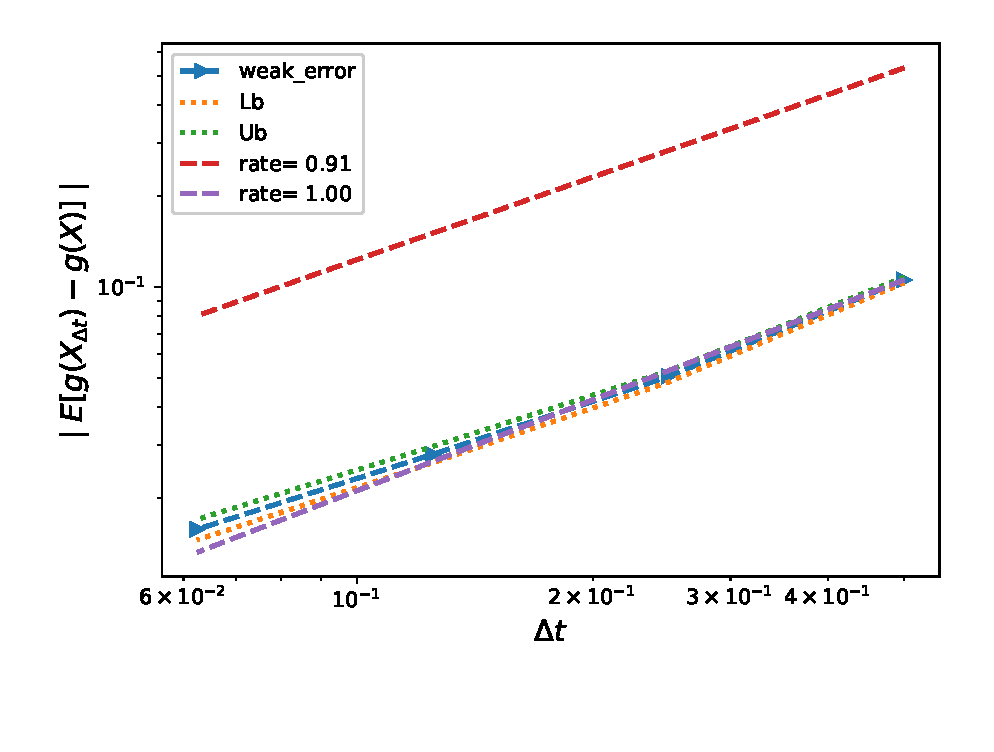
\includegraphics[width=0.4\linewidth]{./figures/binary_weak_error/without_richardson/weak_convergence_order_binary_option_relative_M_10_4}
%		\caption{}
%		\label{fig:sub3}
%	\end{subfigure}%
%	\begin{subfigure}{.35\textwidth}
%		\centering
%		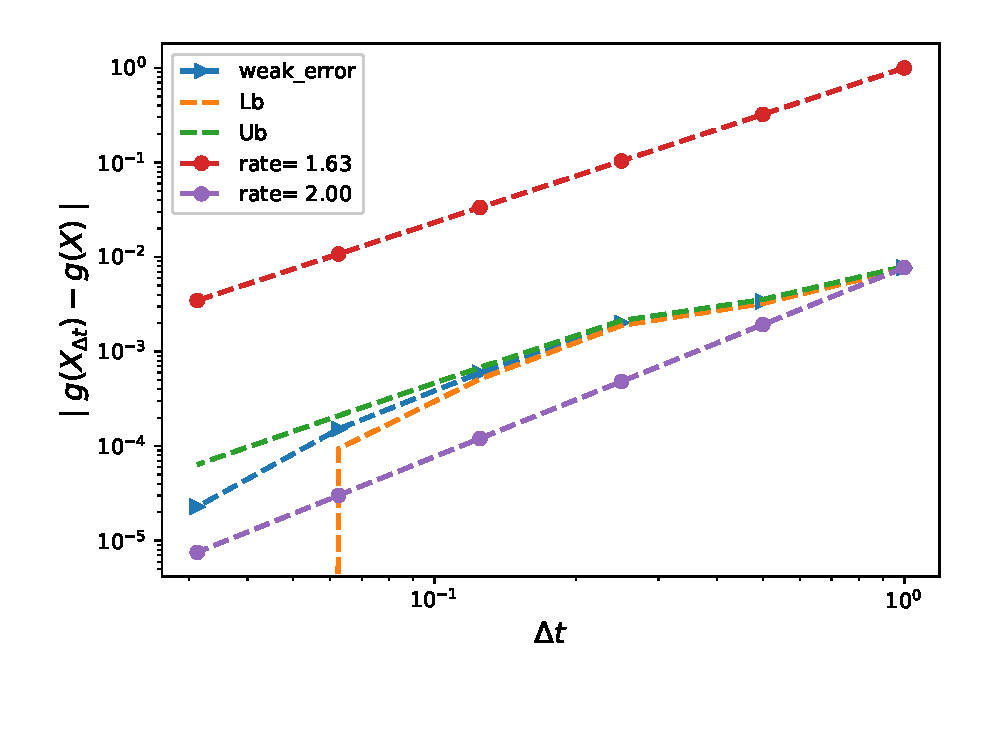
\includegraphics[width=1\linewidth]{./figures/binary_weak_error/with_richardson/weak_convergence_order_binary_richardson_relative_M_5_10_6}
%		\caption{}
%		\label{fig:sub4}
%	\end{subfigure}
	
	\caption{The convergence of the relative weak error  $\mathcal{E}_B(N)$ defined in \ref{eq:total_error}, using MC with $M=10^4$ samples  for the binary option example. The upper and lower bounds are $95\%$ confidence intervals.}
	\label{fig:Weak_rate_binary}
\end{figure}

\FloatBarrier


%\begin{figure}[h!]
%	\centering
%	\begin{subfigure}{.4\textwidth}
%		\centering
%		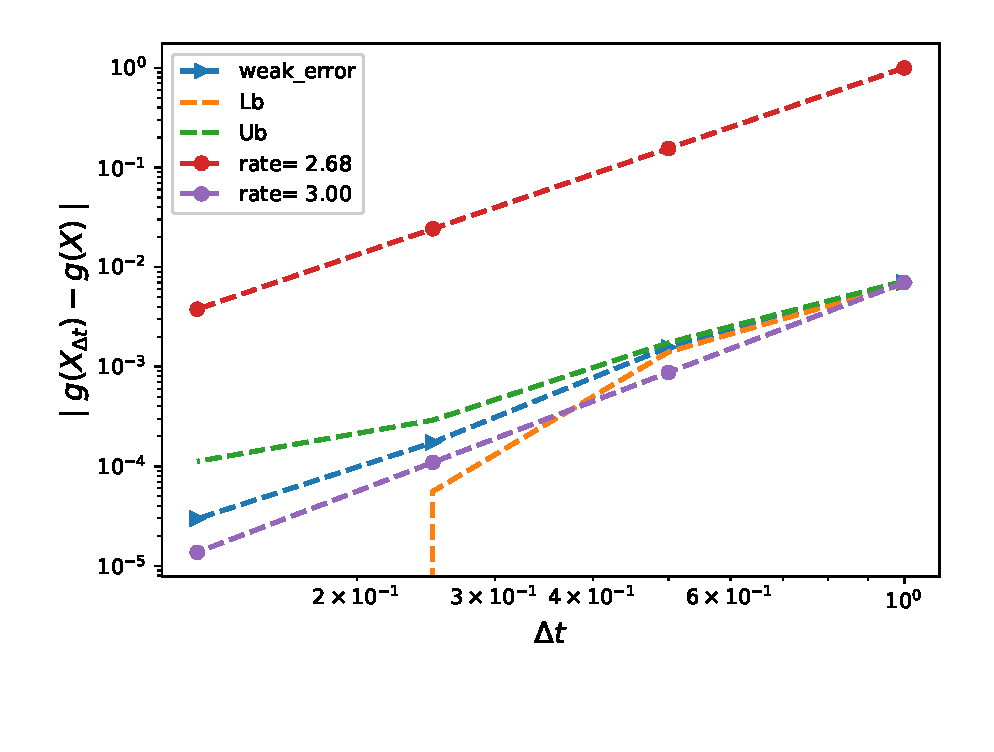
\includegraphics[width=1\linewidth]{./figures/binary_weak_error/with_richardson/weak_convergence_order_binary_richardson_level2_relative_M_5_10_6}
%		\caption{}
%		\label{fig:sub3}
%	\end{subfigure}%
%	\begin{subfigure}{.4\textwidth}
%		\centering
%		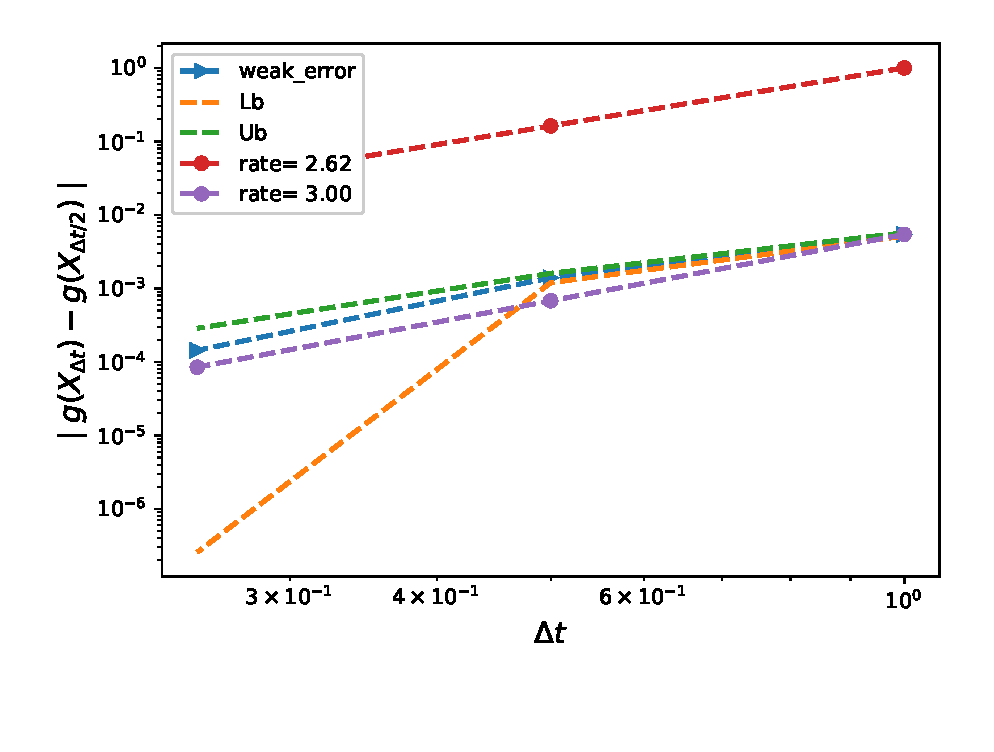
\includegraphics[width=1\linewidth]{./figures/binary_weak_error/with_richardson/weak_convergence_order_differences_binary_richardson_level2_relative_M_5_10_6}
%		\caption{}
%		\label{fig:sub4}
%	\end{subfigure}
%	
%	\caption{The rate of convergence of the weak error for the binary option, with Richardson extraploation (level $2$), using MC with $M=5.10^6$: a) $\abs{\frac{1}{3}\expt{8 g(X_{\Delta t/4}) -6g(X_{\Delta t/2}) +g(X_{\Delta t})}-g(X)}$  b) $\abs{\frac{1}{3}\expt{-8 g(X_{\Delta t/8}) +14g(X_{\Delta t/4})-7 (X_{\Delta t/2}) +g(X_{\Delta t})}}$ }
%	\label{fig:fig:Weak_rate_binary_with_rich_level2}
%\end{figure}
%
%\subsubsection{Comparing relative errors}\label{sec:Comparing relative errors, binary}


%\FloatBarrier
%\begin{table}[h!]
%	\centering
%	\begin{tabular}{l*{6}{c}r}
%		Method \textbackslash  Steps            & $2$ & $4$ & $8$ & $16$ &   \\
%		\hline
%		MISC ($TOL_{\text{MISC}}=5.10^{-1}$)  & $0.4620$ & $0.4404$ & $0.4299$ & $0.4250$  \\
%		MISC ($TOL_{\text{MISC}}=10^{-1}$)  & $0.4620$ & $0.4404$ & $0.4301$ & $0.4250$  \\
%		MISC ($TOL_{\text{MISC}}=5.10^{-2}$)  & $0.4620$ & $0.4403$ & $0.4300$ & $0.4250$  \\
%		MISC ($TOL_{\text{MISC}}=10^{-2}$)  & $0.4620$ & $0.4406$ &  $0.4300$ & $0.4250$  \\
%		MISC ($TOL_{\text{MISC}}=10^{-3}$)  & $0.4620$ & $0.4406$ & $0.4301$  & $0.4254$  \\
%%		MISC ($TOL_{\text{MISC}}=10^{-4}$)  & $0.4620$ & $0.4406$ &  $0.4301$ & $-$  \\
%		\hline
%	%	MC method ($M=10^{5}$)   & $-$ & $-$  & $-$ & $-$ \\		
%		MC method ($M=10^{4}$)   & $  0.4620$ & $    0.4369
%		$  & $      0.4292$ & $  
%		0.4261$ \\	
%		\hline
%	\end{tabular}
%	\caption{Binary option price of the different methods for different number of time steps, without Richardson extrapolation.}
%	\label{table: Binary option price of the different methods for different number of time steps, without Richardson extrapolation.}
%\end{table}

%\begin{table}[h!]
%	\centering
%	\begin{tabular}{l*{6}{c}r}
%		Method \textbackslash  Steps            & $2$ & $4$ & $8$ & $16$  \\
%		\hline
%		MC Bias $(M=10^{4})$  & 	$ \underset{(    
%			0.0412)}{\mathbf{0.0980}}$  & $\underset{( 0.0162)}{\mathbf{ 0.0384
%		}}$  & $\underset{(    0.0085
%	)}{\mathbf{0.0201}}$ & $\underset{(   0.0053)}{\mathbf{   0.0127}}$\\ 
%		
%		MC Statistical error $(M=10^{4})$  &  $\underset{( 5.0e-04)} {\mathbf{1.2e-03}}$  & $\underset{( 5.0e-04)} {\mathbf{1.2e-03}}$ & $\underset{(3.4e-04)} {\mathbf{8.0e-04}}$ & $\underset{( 2.7e-04)} {\mathbf{6.5e-04}}$	\\
%%			MC: Statistical error ($M=10^6$)  &  $\underset{( 5.0e-04)} {\mathbf{1.2e-03}}$  & $\underset{( 5.0e-04)} {\mathbf{1.2e-03}}$ & $\underset{( 5.0e-04)} {\mathbf{1.2e-03}}$ & $\underset{( 5.0e-04)} {\mathbf{1.2e-03}}$	\\
%		\hline
%	\end{tabular}
%	\caption{Bias and statistical errors of MC  for computing binary option price  for different number of time steps, without Richardson extrapolation. The numbers between parentheses are the corresponding absolute errors.}
%	\label{Bias and Statistical errors of MC  for computing Binary option price  for different number of time steps, without Richardson extrapolation. The numbers between parentheses are the corresponding absolute errors.}
%\end{table}
%
%\FloatBarrier
%
%
%
%
%\begin{table}[h!]
%	\centering
%	\begin{tabular}{l*{6}{c}r}
%		Method \textbackslash  Steps            & $2$ & $4$ & $8$ & $16$  \\
%		\hline
%		MISC ($TOL_{\text{MISC}}=5.10^{-1}$)  & $\underset{(2.4e-05)}{\mathbf{\red{1.0e-05}}}$ & $\underset{(0.0035)}{\mathbf{0.0083}}$  & $\underset{(0.0007)}{\mathbf{ 0.0017}}$ &$\underset{(0.0011)}{\mathbf{0.0026}}$ \\
%		MISC ($TOL_{\text{MISC}}=10^{-1}$)   & $\underset{(2.4e-05)}{\mathbf{1.0e-05}}$ & $\underset{(0.0035)}{\mathbf{0.0083}}$ & $\underset{(0.0009)}{\mathbf{\red{0.0021}}}$ & $\underset{(0.0011)}{\mathbf{
%				0.0026}}$ \\
%		MISC ($TOL_{\text{MISC}}=5.10^{-2}$)  & $\underset{(2.4e-05)}{\mathbf{1.0e-05}}$& $\underset{(0.0034)}{\mathbf{0.0081}}$ & $\underset{(0.0008)}{\mathbf{ 0.0019}}$& $\underset{(0.0011)}{\mathbf{
%				0.0026}}$ \\
%		MISC ($TOL_{\text{MISC}}=10^{-2}$)  & $\underset{(2.4e-05)}{\mathbf{1.0e-05}}$ & $\underset{(0.0037)}{\mathbf{\red{0.0088}}}$ & $\underset{(0.0008)}{\mathbf{ 0.0019}}$ & $\underset{(0.0011)}{\mathbf{
%				0.0026}}$ \\
%		MISC ($TOL_{\text{MISC}}=10^{-3}$)  & $\underset{(2.4e-05)}{\mathbf{1.0e-05}}$ & $\underset{(0.0037)}{\mathbf{0.0088}}$& $\underset{(0.0009)}{\mathbf{0.0021}}$& $\underset{(0.0007)}{\mathbf{\red{ 0.0017}}}$ \\
%%			MISC ($TOL_{\text{MISC}}=10^{-4}$)  & $\underset{(2.4e-05)}{\mathbf{1.0e-05}}$ & $\underset{(0.0037)}{\mathbf{0.0088}}$& $\underset{(0.0009)}{\mathbf{0.0021}}$& $\underset{(-)}{\mathbf{ -}}$ \\
%		\hline
%	\end{tabular}
%	\caption{Quadrature error of MISC,  with different tolerances, to compute binary option price for different number of time steps, without Richardson extrapolation. The numbers between parentheses are the corresponding absolute errors. The values marked in red correspond to stable quadrature errors for MISC, and will be used for complexity comparison against MC.}
%	\label{Quadrature error of MISC to compute Binary option price of the different tolerances for different number of time steps, without Richardson extrapolation. The numbers between parentheses are the corresponding absolute errors.}
%\end{table}

%\FloatBarrier
%	\begin{figure}[h!]
%	\centering
%	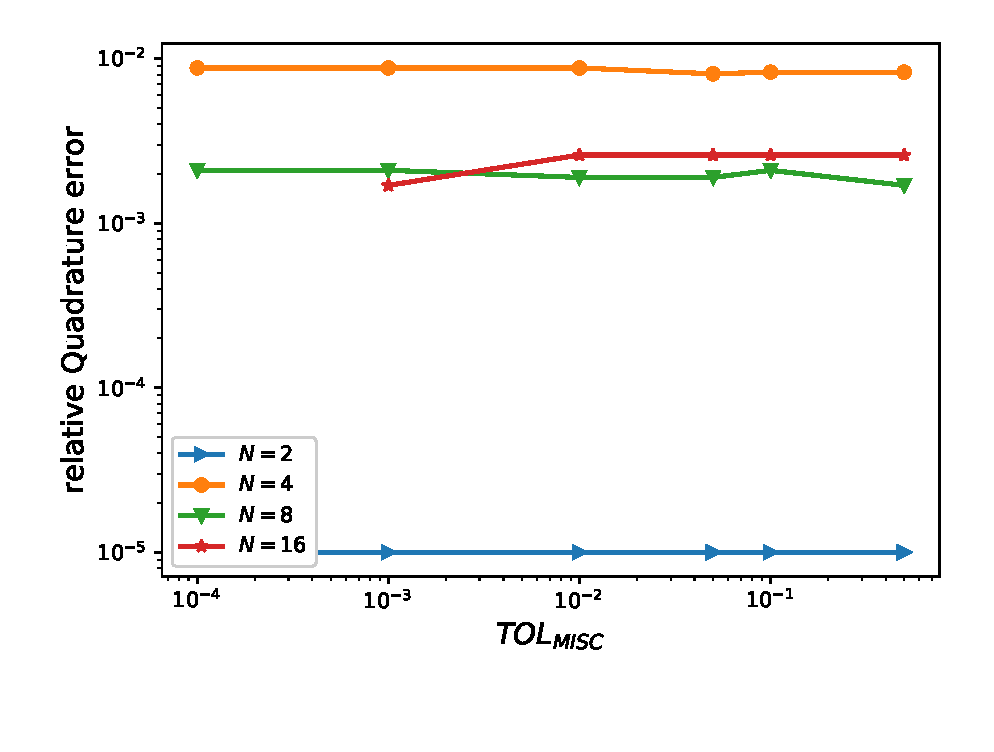
\includegraphics[width=0.4\linewidth]{./figures/Binary_MISC_quadrature_error/relative_quad_error_wrt_MISC_TOL_non_rich}
%	
%	
%	\caption{Relative quadrature error of MISC, with different tolerances, to compute binary option price for different number of time steps, without Richardson extrapolation.}
%	\label{fig:Quadrature_error_non_rich_binary}
%\end{figure}
\FloatBarrier

\begin{table}[h!]
	\centering
	\begin{tabular}{l*{6}{c}r}
		\toprule[1.5pt]
	Method & & Steps  &     \\
	\hline
	        & $4$ & $8$ & $16$  \\
		\hline
%		($TOL_{\text{MISC}}=5.10^{-1}$) 
		ASGQ   & $\underset{(0.04,0.01 )}{\mathbf{0.05}}$ & $\underset{(0.02,0.002)}{\mathbf{ 0.02}}$ & $\underset{(0.01,0.002)}{\mathbf{0.01}}$  \\
%		MISC ($TOL_{\text{MISC}}=10^{-1}$) & $\underset{(0.04,0.01 )}{\mathbf{0.05}}$ & $\underset{(0.02,0.002)}{\mathbf{\red{0.02}}}$ & $\underset{(0.013,0.002)}{\mathbf{0.015}}$   \\
%		MISC ($TOL_{\text{MISC}}=5.10^{-2}$)  & $\underset{(0.04, 0.01)}{\mathbf{0.05}}$ & $\underset{(0.02,0.002)}{\mathbf{0.02}}$ & $\underset{(0.013,0.002)}{\mathbf{0.015}}$  \\
%		MISC ($TOL_{\text{MISC}}=10^{-2}$)  & $\underset{(0.04, 0.01)}{\mathbf{\red{ 0.05}}}$ & $\underset{(0.02,0.002)}{\mathbf{ 0.02}}$ & $\underset{(0.013,0.002)}{\mathbf{0.015}}$    \\
%		MISC ($TOL_{\text{MISC}}=10^{-3}$)   & $\underset{(0.04, 0.01)}{\mathbf{ 0.05}}$  & $\underset{(0.02,0.002)}{\mathbf{ 0.02}}$  & $\underset{(0.013,0.002)}{\mathbf{\red{0.015}}}$\\
		\hline
		MC+root finding   &   $\underset{(0.04,0.04 )}{\mathbf{0.08}}$ & $\underset{(0.02,0.02)}{\mathbf{0.04}}$ & $\underset{(0.01,0.01)}{\mathbf{0.02}}$  \\	
			M(\# MC samples)   & $ 10^1$  & $4 \times 10^1$  & $  10^2$ \\	
		\hline
			MC     & $\underset{(0.05,0.05)}{\mathbf{0.1}}$ & $\underset{(0.025,0.025 )}{\mathbf{0.05}}$ & $\underset{(0.01,0.01 )}{\mathbf{0.02}}$  \\	
			M(\# MC samples)   & $ 10^3$  & $8 \times 10^3$  & $ 5 \times 10^4$ \\	
			\bottomrule[1.25pt]
	\end{tabular}
	\caption{Total relative error of ASGQ, with different tolerances, and MC to compute binary option price for different number of time steps, without Richardson extrapolation. The values between parentheses correspond to the different errors contributing to the total relative error: for ASGQ we report the bias and quadrature errors and for MC we report the bias and the statistical errors. The number of MC samples,$ M$, is chosen to satisfy \eqref{optimal_number_samples}.}
	\label{Total error of MISC and MC to compute Binary option price of the different tolerances for different number of time steps, without Richardson extrapolation. The numbers between parentheses are the corresponding absolute errors.}
\end{table}

\FloatBarrier

\begin{table}[h!]
	\centering
	\begin{tabular}{l*{6}{c}r}
		\toprule[1.5pt]
	Method & & Steps  &     \\
	\hline
		         & $4$ & $8$ & $16$ &   \\
		\hline
%		 ($TOL_{\text{MISC}}=5.10^{-1}$)
		ASGQ   & $0.8$ & $2$ & $9$  \\
%		MISC ($TOL_{\text{MISC}}=10^{-1}$)   & $0.8$ & $\red{9}$ & $49$  \\
%		MISC ($TOL_{\text{MISC}}=5.10^{-2}$)    & $1.3$ & $12$ & $59$  \\
%		MISC ($TOL_{\text{MISC}}=10^{-2}$)   & $\red{2}$ & $14$ & $63$  \\
%		MISC ($TOL_{\text{MISC}}=10^{-3}$)    & $2$ & $34$ & $\red{1090}$  \\
%    	MISC ($TOL_{\text{MISC}}=10^{-4}$)   & $0.3$ & $16$ & $193$ & $-$  \\
		\hline
		MC+root finding     & $0.2$ & $1$ & $9$  \\
		\hline 
		MC     & $0.3$ & $3$ & $29$  \\
%		\hline
%		Ratio of	$\text{(MC+root finding)}/\text{(MISC)}$  & $\red{4.5}$ & $\red{11}$ & $\red{0.13}$  \\
%			Ratio of	$(\text{MC})/(\text{MISC})$ &  $\red{3.5}$ & $\red{11}$ & $\red{0.14}$  \\
				\bottomrule[1.25pt]
	\end{tabular}
	\caption{Comparison of the computational time of  MC and ASGQ, used to compute binary option price  for different number of time steps, without Richardson extrapolation. The average computational time of MC is computed over $10$ runs.}
	\label{Comparsion of the computational time of  MC and MISC, used to compute Binary option price  for different number of time steps, without Richardson extrapolation}
\end{table}



\FloatBarrier
\begin{figure}[h!]
\centering
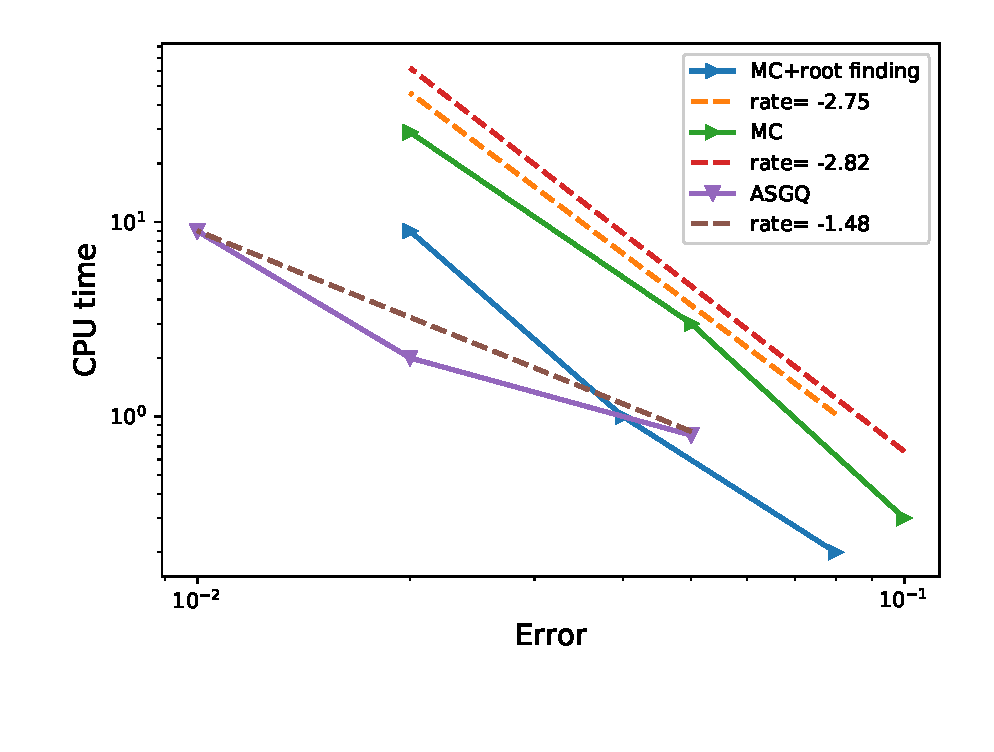
\includegraphics[width=0.4\linewidth]{./figures/Binary_Complexity_rates/error_vs_time}
	\caption{Computational work comparison for ASGQ and MC methods, for the case of binary  option. This plot shows that to achieve a relative error below $1\%$, ASGQ outperforms  MC method in terms of computational time}
	\label{fig:Complexity plot for MC and MISC , Binary, Non rich}
\end{figure}

%\FloatBarrier
%
%\subsubsection*{With Richardson extrapolation (level $1$)}
%
%
%%\FloatBarrier
%%
%%\begin{table}[h!]
%%	\centering
%%	\begin{tabular}{l*{6}{c}r}
%%		Method \textbackslash  Steps            & $1-2$ & $2-4$ & $4-8$ & $8-16$ &   \\
%%		\hline
%%		MISC ($TOL_{\text{MISC}}=5.10^{-1}$)  & $0.4239$ & $0.4188$ & $0.4191$ & $0.4200$  \\
%%		MISC ($TOL_{\text{MISC}}=10^{-1}$)  &$0.4239$ & $0.4188$ &$0.4191$ & $0.4199$  \\
%%		MISC ($TOL_{\text{MISC}}=5.10^{-2}$) & $0.4239$ & $0.4188$ & $0.4190$ & $0.4199$  \\
%%		MISC ($TOL_{\text{MISC}}=10^{-2}$) &$0.4239$ & $0.4192$ & $0.4194$ & $0.4199$  \\
%%%		MISC ($TOL_{\text{MISC}}=10^{-3}$) & $0.4239$ & $0.4192$ & $0.4199$ & $0.4205$  \\
%%%			MISC ($TOL_{\text{MISC}}=10^{-4}$) & $0.4239$ & $0.4193$ & $0.4199$ & $-$  \\
%%		\hline
%%		MC method ($M=5.10^{6}$)   & $ 0.4240$ & $
%%		0.4224$ & $    0.4216$ & $  0.4210$  \\
%%		\hline
%%	\end{tabular}
%%	\caption{Binary option price of the different methods for different number of time steps, with Richardson extrapolation (level $1$).}
%%	\label{table: Binary option price of the different methods for different number of time steps, with Richardson extrapolation (level1).}
%%\end{table}
%%
%%\FloatBarrier
%%\begin{table}[h!]
%%	\centering
%%	\begin{tabular}{l*{6}{c}r}
%%		Method \textbackslash  Steps            & $1-2$ & $2-4$ & $4-8$ & $8-16$  \\
%%		\hline
%%	MC Bias  ($M=5.10^{6}$)&$ \underset{(0.0032)}{\mathbf{0.0077}}$    & $\underset{(    0.0016
%%		)}{\mathbf{0.0039}}$  & $\underset{(0.0008)}{\mathbf{0.0020}}$  & $\underset{(0.0003)}{\mathbf{0.0006}}$\\
%%		MC Statistical error   ($M=5.10^{6}$)   & 	$ \underset{( 4.6e-05  )}{\mathbf{1.1e-04}}$  & $\underset{(3.5e-05)}{\mathbf{ 8.4e-05
%%	}}$  & $\underset{(2.5e-05)}{\mathbf{6.0e-05}}$ & $\underset{(   1.8e-05 )}{\mathbf{  4.2e-05 }}$\\ 
%%		
%%%		MC+root finding: Statistical error ($M=10^3$)     & 	$ \underset{( 3.5e-03  )}{\mathbf{8.3e-03}}$  & $\underset{(2.8e-03)}{\mathbf{ 6.6e-03
%%%		}}$  & $\underset{(1.8e-03)}{\mathbf{4.3e-03}}$ & $\underset{(  1.2e-03 )}{\mathbf{  2.9e-03 }}$\\ 
%%%		
%%		\hline
%%	\end{tabular}
%%	\caption{Bias and statistical errors of MC  for computing binary option price  for different number of time steps, with Richardson extrapolation (level $1$). The numbers between parentheses are the corresponding absolute errors.}
%%	\label{Bias and Statistical errors of MC  for computing Binary option price  for different number of time steps, with Richardson extrapolation (level $1$). The numbers between parentheses are the corresponding absolute errors.}
%%\end{table}
%
%%\FloatBarrier
%%
%%
%%
%%\begin{table}[h!]
%%	\centering
%%	\begin{tabular}{l*{6}{c}r}
%%		Method \textbackslash  Steps            & $1-2$ & $2-4$ & $4-8$ & $8-16$  \\
%%		\hline
%%		MISC ($TOL_{\text{MISC}}=5.10^{-1}$)  & $\underset{(   1.0e-04)}{\mathbf{ \red{2.4e-04}}}$ & $\underset{(3.6e-03)}{\mathbf{8.6e-03}}$  & $\underset{(2.5e-03)}{\mathbf{5.9e-03}}$ &$\underset{(1.0e-03)}{\mathbf{2.4e-03}}$ \\
%%		MISC ($TOL_{\text{MISC}}=10^{-1}$)   & $\underset{(   1.0e-04)}{\mathbf{ 2.4e-04}}$ & $\underset{(3.6e-03)}{\mathbf{8.6e-03}}$  & $\underset{(2.5e-03)}{\mathbf{5.9e-03}}$ &$\underset{(   1.1e-04)}{\mathbf{ \red{2.6e-03}}}$ \\
%%		MISC ($TOL_{\text{MISC}}=5.10^{-2}$)  & $\underset{(   1.0e-04)}{\mathbf{ 2.4e-04}}$ & $\underset{(3.6e-03)}{\mathbf{8.6e-03}}$ & $\underset{(2.6e-03)}{\mathbf{6.2e-03}}$ &$\underset{(   1.1e-04)}{\mathbf{ 2.6e-03}}$ \\
%%		MISC ($TOL_{\text{MISC}}=10^{-2}$)  & $\underset{(   1.0e-04)}{\mathbf{ 2.4e-04}}$ & $\underset{(3.2e-03)}{\mathbf{\red{7.6e-03}}}$  & $\underset{(2.2e-03)}{\mathbf{\red{5.2e-03}}}$ &$\underset{(   1.1e-04)}{\mathbf{ 2.6e-03}}$\\
%%%		MISC ($TOL_{\text{MISC}}=10^{-3}$)  & $\underset{(   1.0e-04)}{\mathbf{ 2.4e-04}}$ & $\underset{(3.2e-03)}{\mathbf{7.6e-03}}$  & $\underset{(1.7e-03)}{\mathbf{4.0e-03}}$ &$\underset{(   5.e-04)}{\mathbf{1.2e-03}}$ \\
%%%	MISC ($TOL_{\text{MISC}}=10^{-4}$)  & $\underset{(   1.0e-04)}{\mathbf{ 2.4e-04}}$ & $\underset{(3.1e-03)}{\mathbf{7.4e-03}}$  & $\underset{(1.7e-03)}{\mathbf{4.0e-03}}$ &$\underset{()}{\mathbf{}}$ \\
%%		\hline
%%	\end{tabular}
%%	\caption{Quadrature error of MISC, with different tolerances,  to compute binary option price for different number of time steps, with Richardson extrapolation (level $1$). The numbers between parentheses are the corresponding absolute errors. The values marked in red correspond to stable quadrature errors for MISC, and will be used for complexity comparison against MC.}
%%	\label{Quadrature error of MISC to compute Binary option price of the different tolerances for different number of time steps, with Richardson extrapolation (level $1$). The numbers between parentheses are the corresponding absolute errors.}
%%\end{table}
%%
%%
%%\FloatBarrier
%%	\begin{figure}[h!]
%%	\centering
%%	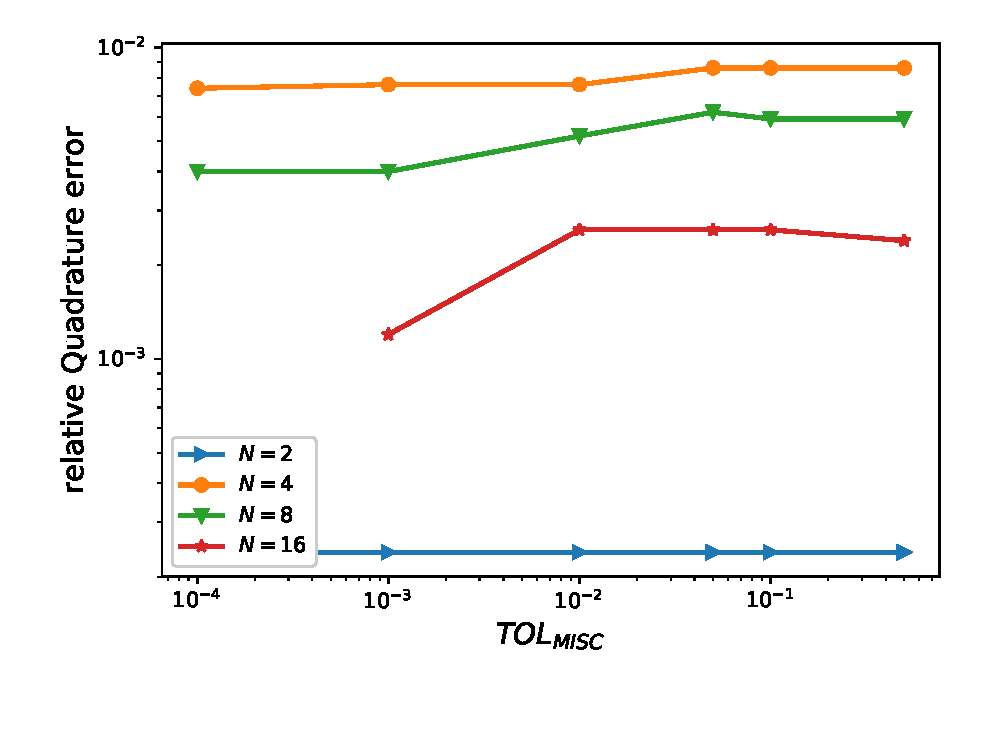
\includegraphics[width=0.4\linewidth]{./figures/Binary_MISC_quadrature_error/relative_quad_error_wrt_MISC_TOL_with_rich}
%%	
%%	
%%	\caption{Relative quadrature error of MISC, with different tolerances, to compute binary option price of the different tolerances for different number of time steps, with Richardson extrapolation.}
%%	\label{fig:Quadrature_error_with_rich_binary}
%%\end{figure}
%
%\FloatBarrier
%
%\begin{table}[h!]
%	\centering
%	\begin{tabular}{l*{6}{c}r}
%		\toprule[1.5pt]
%	Method & & Steps  &     \\
%	\hline
%		        & $2-4$ & $4-8$ & $8-16$  \\
%		\hline
%		MISC ($TOL_{\text{MISC}}=5.10^{-1}$)  & $\underset{(0.004,0.009)}{\mathbf{0.013}}$ & $\underset{(0.002,0.006)}{\mathbf{0.008}}$ & $\underset{(0.0006,0.0016)}{\mathbf{0.002}}$  \\
%%		MISC ($TOL_{\text{MISC}}=10^{-1}$)  &    $\underset{(0.004,0.009)}{\mathbf{0.013}}$ & $\underset{(0.002,0.006)}{\mathbf{0.008}}$ & $\underset{(0.0006,0.0026)}{\mathbf{\red{0.003}}}$  \\
%%		MISC ($TOL_{\text{MISC}}=5.10^{-2}$) & $\underset{(0.004,0.009)}{\mathbf{0.013}}$ & $\underset{(0.002,0.006)}{\mathbf{0.008}}$ & $\underset{(0.0006,0.0026)}{\mathbf{0.003}}$  \\
%%		MISC ($TOL_{\text{MISC}}=10^{-2}$)   & $\underset{(0.004,0.008)}{\mathbf{\red{0.012}}}$ & $\underset{(0.002,0.005)}{\mathbf{\red{0.007}}}$ & $\underset{(0.0006,0.0026)}{\mathbf{0.003}}$  \\
%%		MISC ($TOL_{\text{MISC}}=10^{-3}$) &   $\mathbf{0.0079}$ & $\mathbf{0.0115}$ & $\mathbf{0.0060}$ & $\mathbf{0.0018}$  \\
%%
%%	MISC ($TOL_{\text{MISC}}=10^{-4}$) &   $\mathbf{0.0079}$ & $\mathbf{0.0113}$ & $\mathbf{0.0060}$ & $\mathbf{-}$  \\
%		\hline
%		MC+root finding   & $\underset{(0.004,)}{\mathbf{\red{0.008}}}$ & $\underset{(0.002,)}{\mathbf{\red{0.004}}}$ & $\underset{(0.0006,)}{\mathbf{\red{0.001}}}$  \\	
%			MC     & $\mathbf{\red{0.0116}}$ & $\mathbf{\red{0.0073}}$ & $\mathbf{\red{0.0029}}$  \\	
%			\bottomrule[1.25pt]
%	\end{tabular}
%	\caption{Total relative error of MISC, with different tolerances, and MC to compute binary option price for different number of time steps, with Richardson extrapolation (level $1$).  The values marked in red, for MISC method, correspond to the total relative errors associated with  stable quadrature errors for MISC, and will be used for complexity comparison against MC.}
%	\label{Total error of MISC and MC to compute Binary option price of the different tolerances for different number of time steps, with Richardson extrapolation (level $1$). The numbers between parentheses are the corresponding absolute errors.}
%\end{table}
%
%
%
%\FloatBarrier
%
%
%\begin{table}[h!]
%	\centering
%	\begin{tabular}{l*{6}{c}r}
%		\toprule[1.5pt]
%	Method & & Steps  &     \\
%	\hline
%		   & $2-4$ & $4-8$ & $8-16$ &   \\
%		\hline
%		MISC ($TOL_{\text{MISC}}=5.10^{-1}$) & $1$ & $4$ & $9$  \\
%%		MISC ($TOL_{\text{MISC}}=10^{-1}$) & $1$ & $8$ & $\red{42}$  \\
%%		MISC ($TOL_{\text{MISC}}=5.10^{-2}$)  & $1$ & $10$ & $72$  \\
%%		MISC ($TOL_{\text{MISC}}=10^{-2}$)   & $\red{4}$ & $\red{15}$ & $78$  \\
%%		MISC ($TOL_{\text{MISC}}=10^{-3}$)   &$0.3$ & $4$ & $100$ & $2253$  \\
%%			MISC ($TOL_{\text{MISC}}=10^{-4}$)   &$0.3$ & $68$ & $392$ & $$  \\
%		\hline
%		MC+root finding method      & $\red{48}$ & $\red{62}$ & $\red{122 }$  \\
%			MC    & $\red{12}$ & $\red{23}$ & $\red{147}$  \\
%%		\hline
%%			Ratio of	$\text{(MC+root finding)}/\text{(MISC)}$  & $\red{12}$ & $\red{4.1}$ & $\red{2.9}$  \\
%%		Ratio of	$(\text{MC})/(\text{MISC})$ & $\red{3}$ & $\red{1.5}$ & $\red{3.5}$  \\
%		\bottomrule[1.25pt]
%	\end{tabular}
%	\caption{Comparison of the computational time of  MC and MISC, used to compute binary option price  for different number of time steps, with Richardson extrapolation (level $1$). The average computational time of MC is computed over $10$ runs.}
%	\label{Comparsion of the computational time of  MC and MISC, used to compute Binary option price  for different number of time steps, with Richardson extrapolation (level $1$)}
%\end{table}
%
%\FloatBarrier
%	\begin{figure}[h!]
%\centering
%\includegraphics[width=0.4\linewidth]{./figures/Binary_Complexity_rates/error_vs_time_rich}
%
%\caption{Complexity plot for MC and MISC for the case with Richardson extrapolation.}
%\label{fig:Complexity plot for MC and MISC , Binary, with rich}
%\end{figure}
%
%
%
%
%
%
%\FloatBarrier
%
%\begin{figure}[h!]
%\centering
%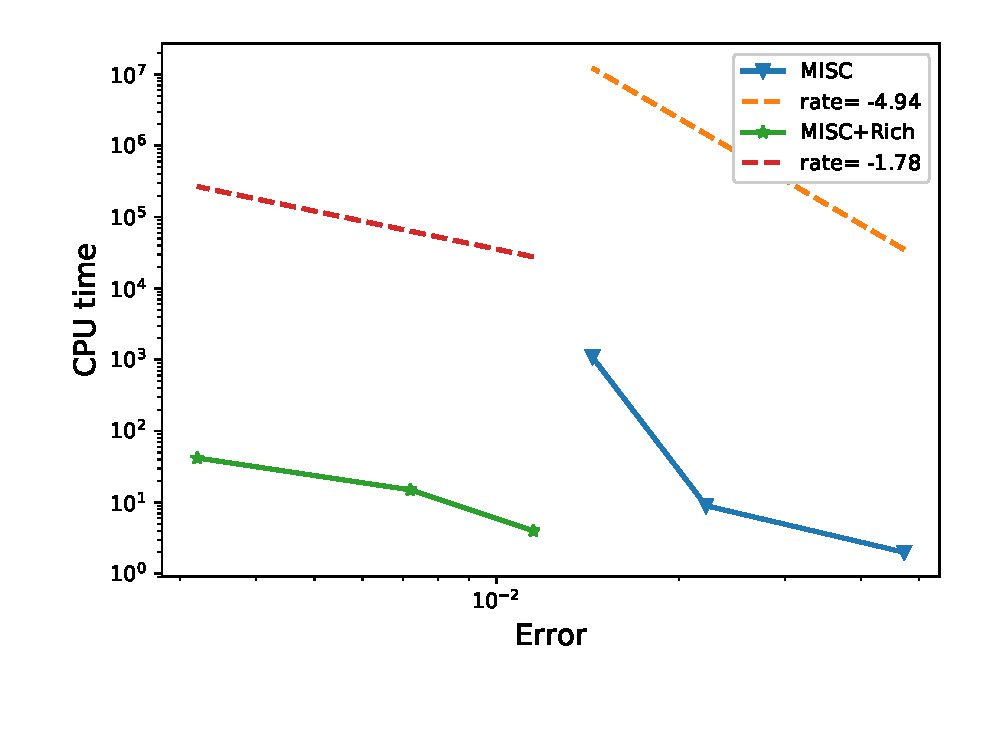
\includegraphics[width=0.4\linewidth]{./figures/Binary_Complexity_rates/error_vs_time_comparison}
%
%\caption{Complexity plot for MISC without and with Richardson extrapolation, for the binary option.}
%\label{fig:Complexity plot for MC and MISC , Binary, comparison}
%\end{figure}
%
%\FloatBarrier
%


%In the following, we compare the  relative errors for the binary option example under Black-Scholes model (see Tables (\ref{Relative error of the binary option price of the different tolerances for different number of time steps.}, \ref{Relative error of Call option price of the different tolerances for different number of time steps, using Richardson extrapolation (level $1$)})). We report the results for $2$ scenarios: i) Without using Richardson extrapolation, ii) Using level $1$ Richardson extrapoaltion.  You may see appendix \ref{appendix:Call prices for different methods_binary} for the values of binary option prices.
%
%Given the normalized bias computed by MC method (See Section \ref{sec:Weak error plots_binary}) (reported as bold values in the tables), we report in red in each table the smallest tolerance that MISC required to get below that relative bias (I do not put values for smaller tolerances, once the required bias is reached).
%
%From the tables (\ref{Relative error of the binary option price of the different tolerances for different number of time steps.}, \ref{Relative error of Call option price of the different tolerances for different number of time steps, using Richardson extrapolation (level $1$)})), we may observe that to get a relative error below $1\%$, we need around $16$ time steps for the case without Richardson extrapolation compared to only using $1$ time step in the coarse level for the case of level $1$ Richardson extraplation. 



%\begin{table}[h!]
%	\centering
%	\begin{tabular}{l*{5}{c}r}
%		Method \textbackslash  Steps    &$1-2$        & $2-4$ & $4-8$ & $8-16$  \\
%		\hline
%		MISC ($TOL_{\text{MISC}}=5.10^{-1}$)  &$\red{0.0076}$ & $0.0045$ & $0.0031$ & $0.0017$  \\
%		MISC ($TOL_{\text{MISC}}=10^{-2}$)  &$-$ & $\red{0.0036}$ & $0.0031$ & $0.0014$  \\
%		MISC ($TOL_{\text{MISC}}=10^{-3}$) & $-$ & $-$ & $  \red{0.0021}$ & $\red{0.0005}$   \\
%		MC method ($M=5.10^{6}$)&$ \mathbf{0.0077}$    & $\mathbf{0.0039}$  & $\mathbf{0.0020}$  & $\mathbf{0.0006}$ \\
%		\hline
%	\end{tabular}
%	\caption{Relative error of the binary option price of the different tolerances for different number of time steps, using Richardson extrapolation (level $1$)}
%	\label{Relative error of binary option price of the different tolerances for different number of time steps, using Richardson extrapolation (level $1$)}
%\end{table}


\FloatBarrier
\subsubsection{Results for the single call option example}\label{sec:Results for the call option example}
In this case, the integrand $h(\mathbf{z}_{-1})$ is given by

\begin{align}\label{smoothed_integrand_call_opt_2}
h(\mathbf{z}_{-1})&= \int_{\rset}  \max \left(\Psi \circ \Phi(T;z_1,\mathbf{z}_{-1})-K,0\right) \frac{1}{\sqrt{2 \pi}} \operatorname{exp}(-z_1^2/2) dz_1 \PERIOD
\end{align}
We get the kink point by running Newton iteration with a precision of $10^{-10}$. We  decompose the total integration domain $\rset$  into sub-domains such that the integrand is smooth in the interior of  each sub-domain and such that the kink is located along the boundary of these areas. The total integral is then given as the sum of the separate integrals, \ie
\begin{align}
	h(\mathbf{z}_{-1}) &:=  \int_{\rset} \max \left(\Psi \circ \Phi(T;z_1,\mathbf{z}_{-1})-K,0\right) \frac{1}{\sqrt{2 \pi}} \operatorname{exp}(-z_1^2/2) dy \\ \nonumber
	&=\int_{-\infty}^{y^{\ast}} \max \left(\Psi \circ \Phi(T;z_1,\mathbf{z}_{-1})-K,0\right) \frac{1}{\sqrt{2 \pi}} \operatorname{exp}(-z_1^2/2) dz_1\\ \nonumber
	&+\int_{y^{\ast}}^{\infty} \max \left(\Psi \circ \Phi(T;z_1,\mathbf{z}_{-1})-K,0\right) \frac{1}{\sqrt{2 \pi}} \operatorname{exp}(-z_1^2/2) dz_1,
\end{align}
where we use Gauss-Laguerre quadrature with $\beta$ points to get each part.

The parameters that we used in our numerical experiments are: $T=1$, $\sigma=0.4$ and $S_0=K=100$. The exact value of this case is $15.85193755$.

Figure \ref{fig:Weak_rate_call_beta_32} shows the estimated   weak error  for the case without Richardson extrapolation, and we report the results for comparing MC and ASGQ in Tables \ref{Total error of MISC and MC to compute Call option price of the different tolerances for different number of time steps, without Richardson extrapolation. The numbers between parentheses are the corresponding absolute errors.} and \ref{Comparsion of the computational time of  MC and MISC, used to compute Call option price  for different number of time steps, without Richardson extrapolation}, and Figure \ref{fig:Complexity plot for MC and MISC , Call non rich}. Our numerical experiments show that ASGQ  requires approximately $5\%$ of the work of MC  to achieve a total relative error of around $0.9\%$.



%\subsubsection*{$\beta=10$}
%From figure \ref{fig:Weak_rate_call_without_rich}, we see that we get a weak error of order $\Delta t$. From figure \ref{fig:fig:Weak_rate_call_with_rich}, we observe that we get a weak error of order $\Delta t^2$ (if eliminate the  last point having a wide confidence interval point). From figure \ref{fig:Weak_rate_call_with_rich_level2}, we observe that we get an almost constant weak error, with that constant being the smallest cpmpared to without and with level $1$ Ricardson extrapolation. The upper and lower bounds are $95\%$ confidence interval.

%\begin{figure}[h!]
%	\centering
%	\begin{subfigure}{.35\textwidth}
%		\centering
%		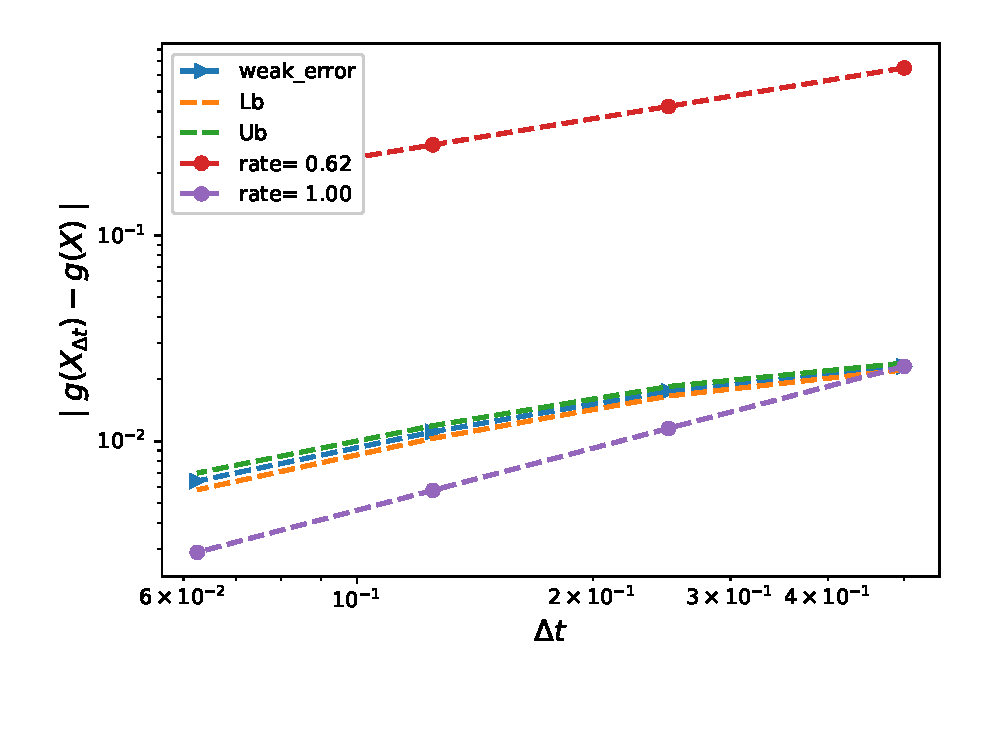
\includegraphics[width=1\linewidth]{./figures/weak_error_rates_call/Beta_10/without_richardson/weak_convergence_order_call_option_relative_M_10_5}
%		\caption{}
%		\label{fig:sub3}
%	\end{subfigure}%
%	\begin{subfigure}{.35\textwidth}
%		\centering
%		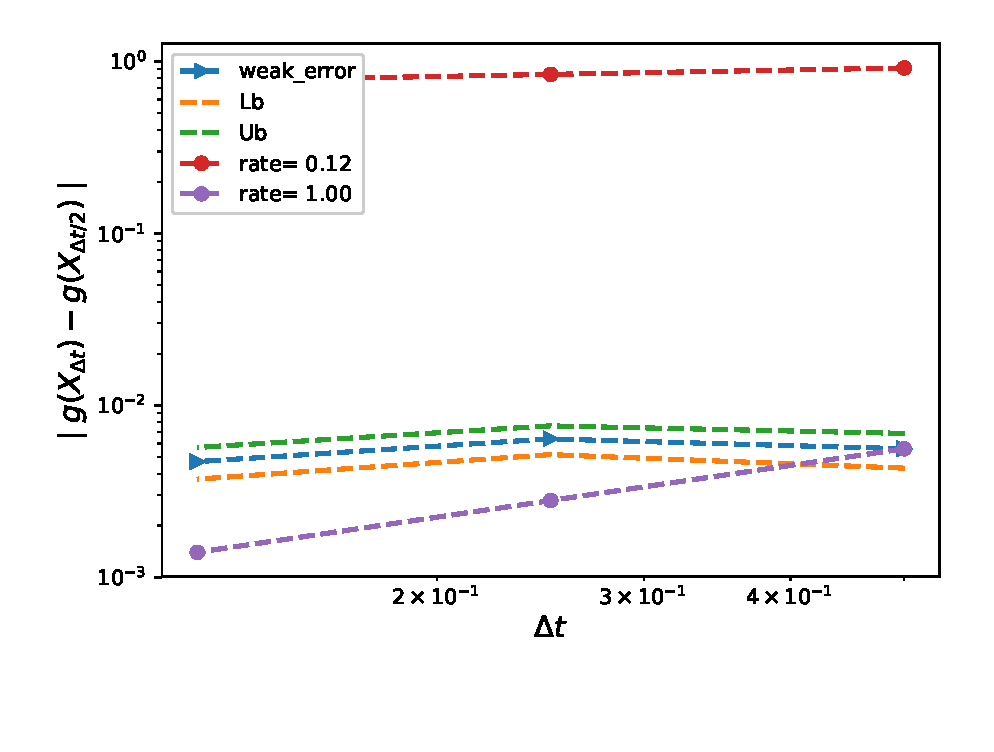
\includegraphics[width=1\linewidth]{./figures/weak_error_rates_call/Beta_10/without_richardson/weak_convergence_order_differences_call_option_relative_M_10_5}
%		\caption{}
%		\label{fig:sub4}
%	\end{subfigure}
%	
%	\caption{The rate of convergence of the weak error for the call option, without Richardson extraploation, using MC with $M=10^5$: a) $\abs{\expt{g(X_{\Delta t})}-g(X)}$  b) $\abs{\expt{g(X_{\Delta t})-g(X_{\Delta t/2})}}$ }
%	\label{fig:Weak_rate_call_without_rich}
%\end{figure}
%\begin{figure}[h!]
%	\centering
%	\begin{subfigure}{.35\textwidth}
%		\centering
%		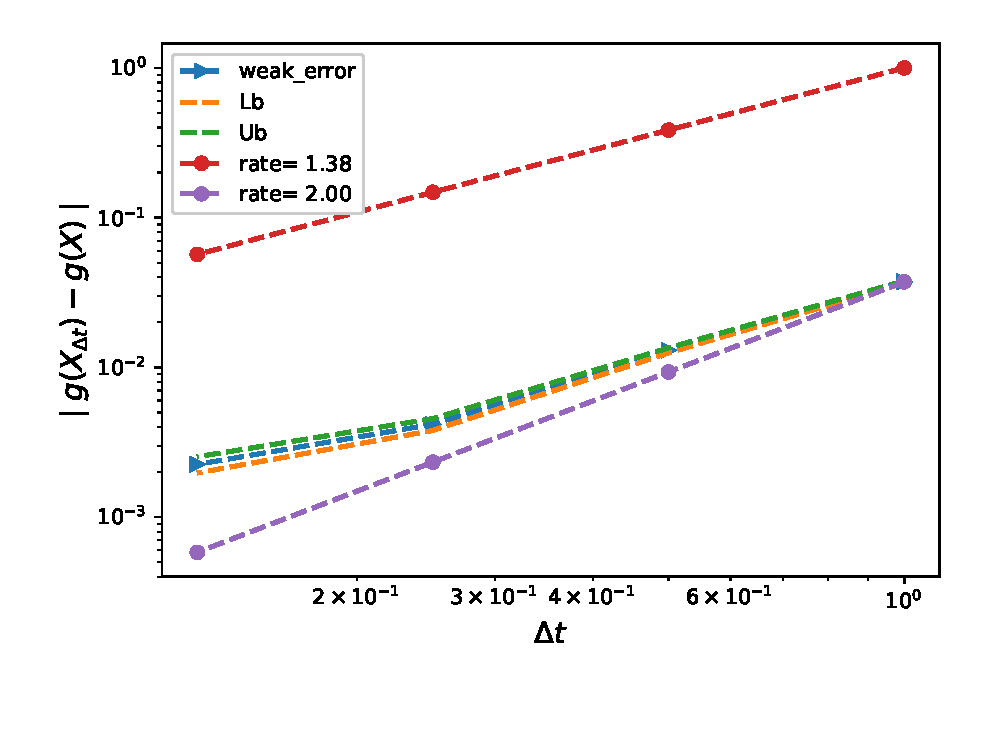
\includegraphics[width=1\linewidth]{./figures/weak_error_rates_call/Beta_10/with_richardson/weak_convergence_order_call_richardson_relative_M_10_6}
%		\caption{}
%		\label{fig:sub3}
%	\end{subfigure}%
%	\begin{subfigure}{.35\textwidth}
%		\centering
%		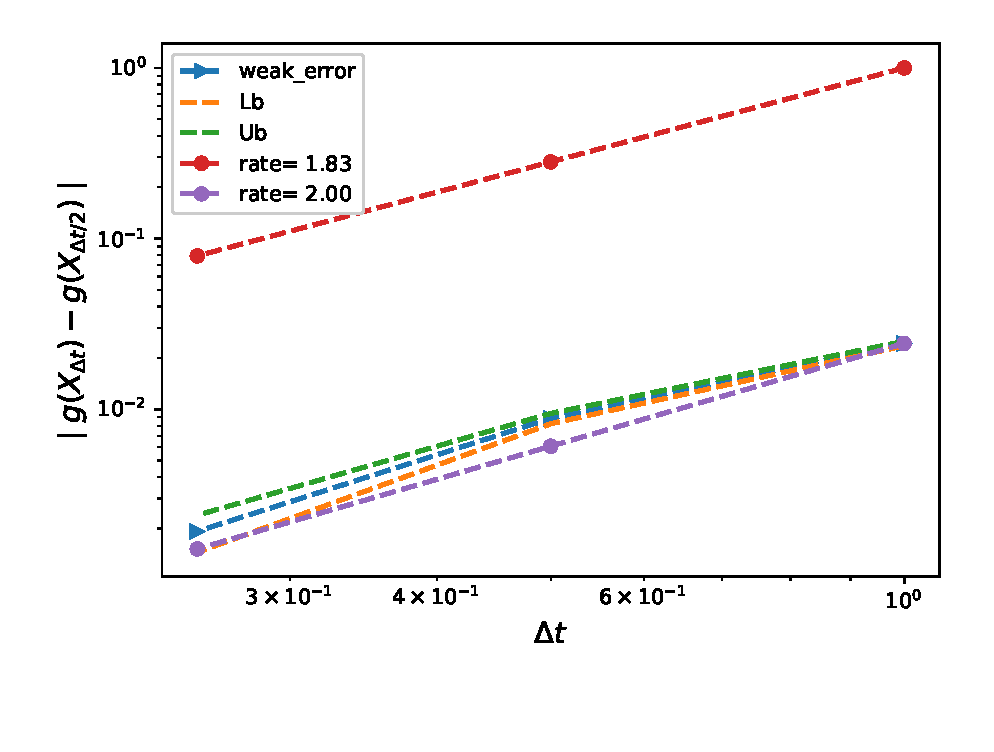
\includegraphics[width=1\linewidth]{./figures/weak_error_rates_call/Beta_10/with_richardson/weak_convergence_order_differences_call_richardson_relative_M_10_6}
%		\caption{}
%		\label{fig:sub4}
%	\end{subfigure}
%	
%	\caption{The rate of convergence of the weak error for the  call option with Richardson extraploation, using MC with $M=10^6$: a) $\abs{\expt{2 g(X_{\Delta t/2}) -g(X_{\Delta t})}-g(X)}$  b) $\abs{\expt{3 g(X_{\Delta t/2})-g(X_{\Delta t})-2 g(X_{\Delta t/4})}}$ }
%	\label{fig:fig:Weak_rate_call_with_rich}
%\end{figure}



%\begin{figure}[h!]
%	\centering
%	\begin{subfigure}{.4\textwidth}
%		\centering
%		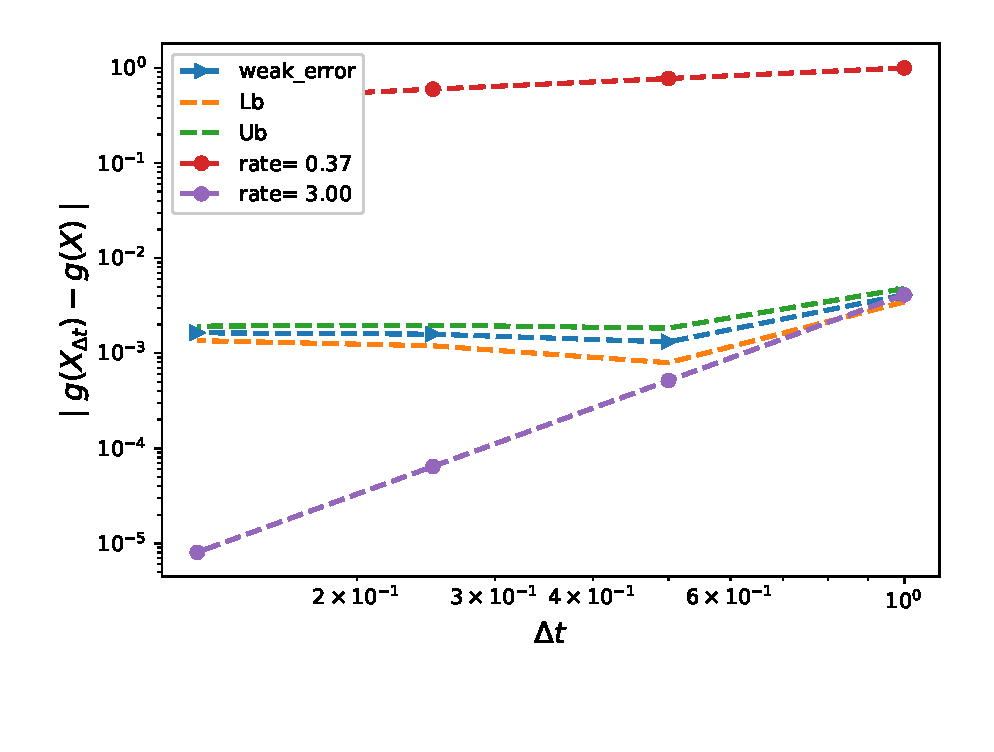
\includegraphics[width=1\linewidth]{./figures/weak_error_rates_call/Beta_10/with_richardson/weak_convergence_order_Call_richardson_level2_relative_M_10_6}
%		\caption{}
%		\label{fig:sub3}
%	\end{subfigure}%
%	\begin{subfigure}{.4\textwidth}
%		\centering
%		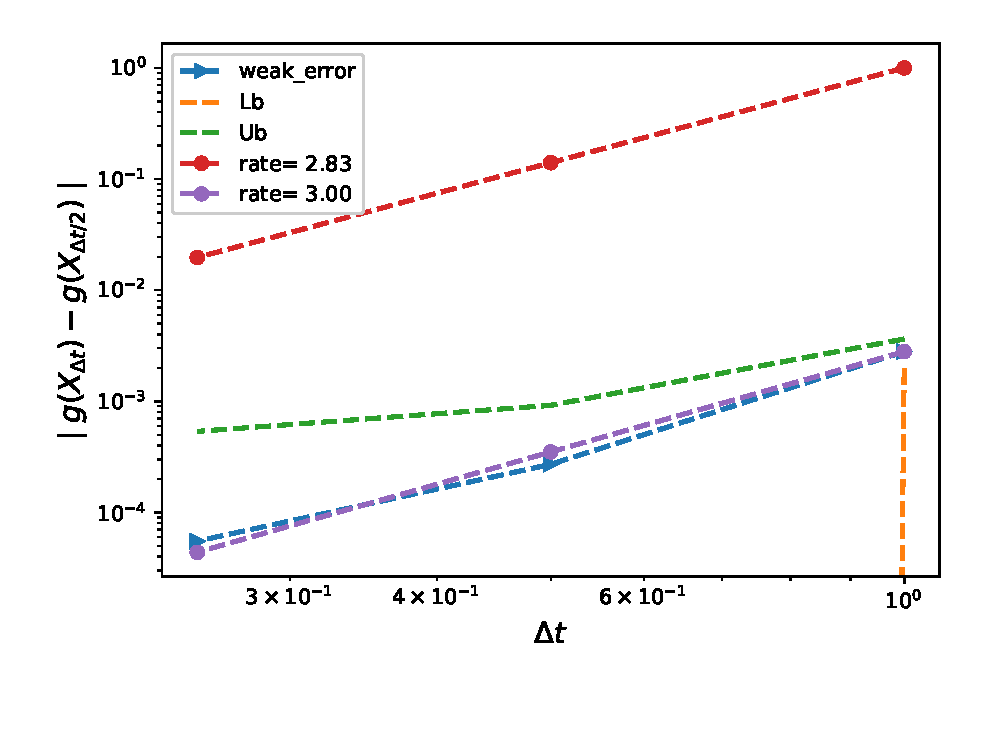
\includegraphics[width=1\linewidth]{./figures/weak_error_rates_call/Beta_10/with_richardson/weak_convergence_order_differences_Call_richardson_level2_relative_M_10_6}
%		\caption{}
%		\label{fig:sub4}
%	\end{subfigure}
	
%	\caption{The rate of convergence of the weak error for the  call option with Richardson extraploation (level 2), using MC with $M=10^6$: a) $\abs{\frac{1}{3}\expt{8 g(X_{\Delta t/4}) -6g(X_{\Delta t/2}) +g(X_{\Delta t})}-g(X)}$  b) $\abs{\frac{1}{3}\expt{-8 g(X_{\Delta t/8}) +14g(X_{\Delta t/4})-7 (X_{\Delta t/2}) +g(X_{\Delta t})}}$}
%	\label{fig:Weak_rate_call_with_rich_level2}
%\end{figure}


%\FloatBarrier
%\subsubsection*{$\beta=32$}

\begin{figure}[h!]
	\centering
%	\begin{subfigure}{.35\textwidth}
%		\centering
		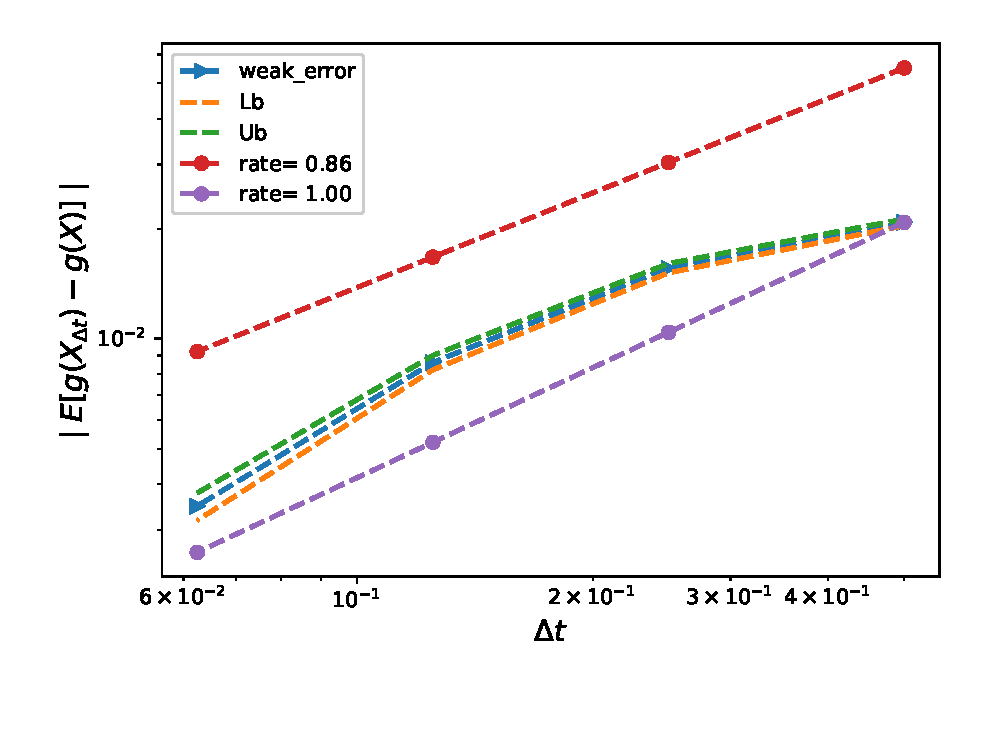
\includegraphics[width=0.5\linewidth]{./figures/weak_error_rates_call/Beta_32/without_rich/weak_convergence_order_call_option_relative_M_4_10_5}
%		\caption{}
%		\label{fig:sub3}
%	\end{subfigure}%
%	\begin{subfigure}{.35\textwidth}
%		\centering
%		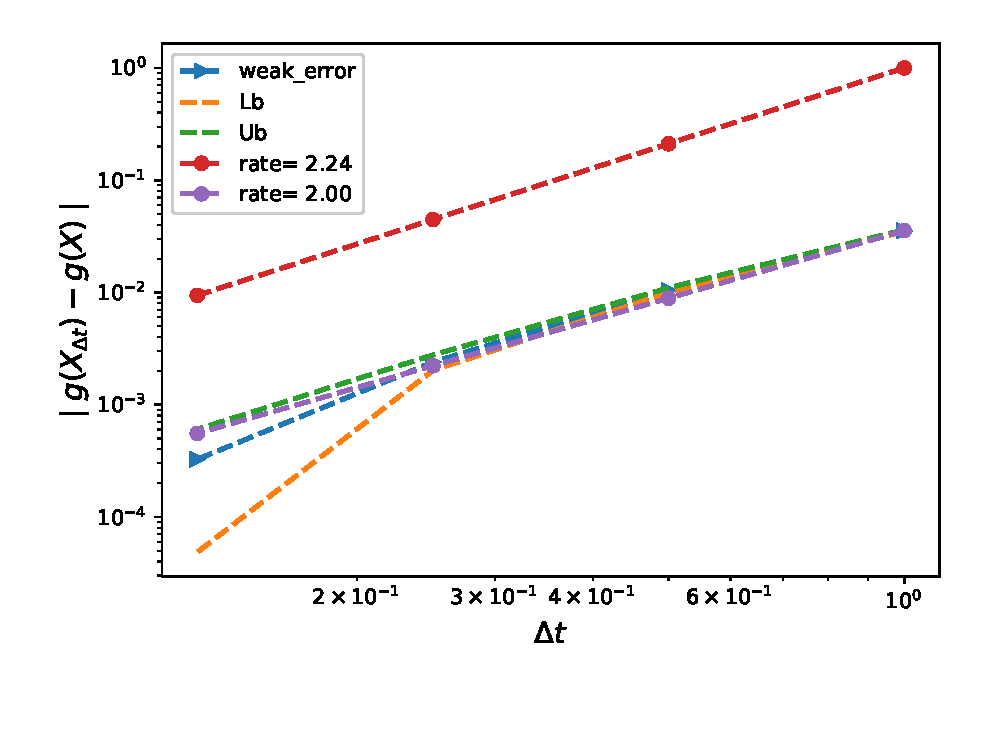
\includegraphics[width=1\linewidth]{./figures/weak_error_rates_call/Beta_32/with_rich/weak_convergence_order_call_richardson_relative}
%		\caption{}
%		\label{fig:sub4}
%	\end{subfigure}
	
	\caption{The convergence of the relative weak error  $\mathcal{E}_B(N)$ defined in \ref{eq:total_error}, using MC with $M=4 \times 10^5$ samples  for the call option example. The upper and lower bounds are $95\%$ confidence intervals.}
	\label{fig:Weak_rate_call_beta_32}
\end{figure}

%\begin{figure}[h!]
%	\centering
%	\begin{subfigure}{.35\textwidth}
%		\centering
%		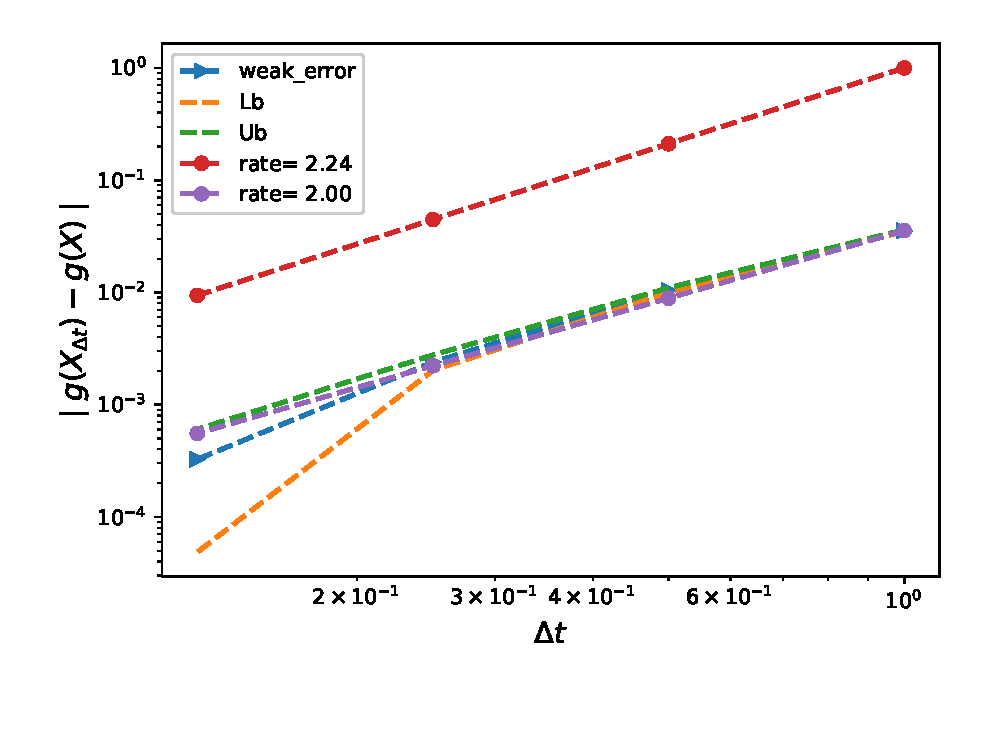
\includegraphics[width=1\linewidth]{./figures/weak_error_rates_call/Beta_32/with_rich/weak_convergence_order_call_richardson_relative}
%		\caption{}
%		\label{fig:sub3}
%	\end{subfigure}%
%	\begin{subfigure}{.35\textwidth}
%		\centering
%		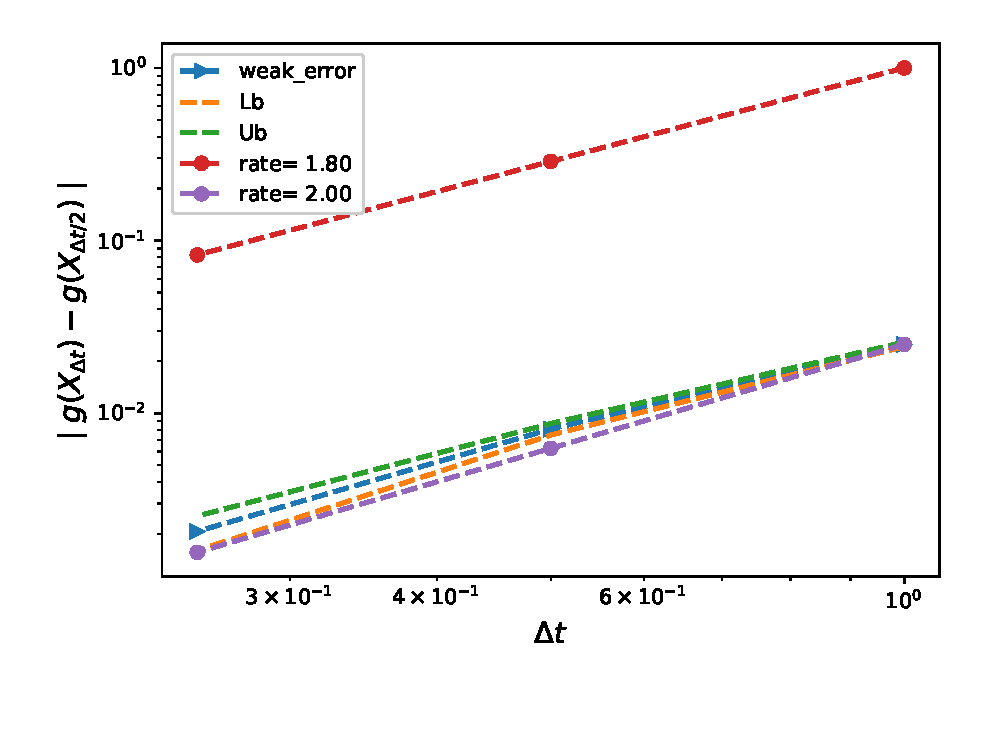
\includegraphics[width=1\linewidth]{./figures/weak_error_rates_call/Beta_32/with_rich/weak_convergence_order_differences_call_richardson_relative}
%		\caption{}
%		\label{fig:sub4}
%	\end{subfigure}
%	
%	\caption{The rate of convergence of the weak error for the  call option with Richardson extraploation (level 1), using MC with $M=5.10^6$: a)   b) $\abs{\expt{3 g(X_{\Delta t/2})-g(X_{\Delta t})-2 g(X_{\Delta t/4})}}$}
%	\label{fig:Weak_rate_call_with_rich_level1_beta_32}
%\end{figure}


%\begin{figure}[h!]
%	\centering
%	\begin{subfigure}{.4\textwidth}
%		\centering
%		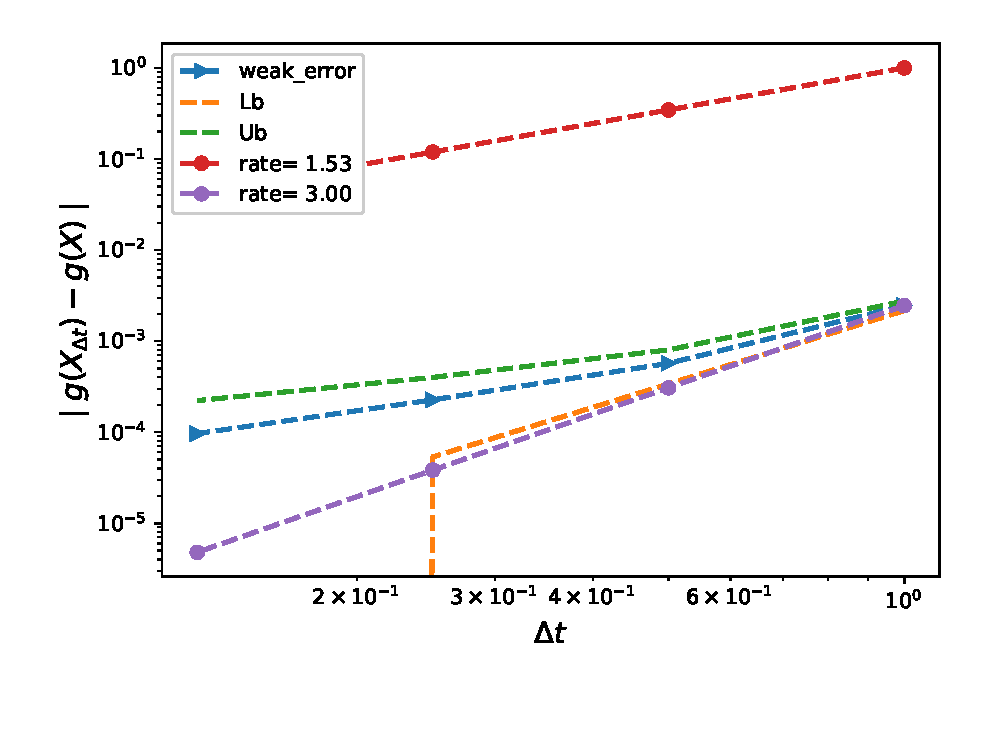
\includegraphics[width=1\linewidth]{./figures/weak_error_rates_call/Beta_32/with_rich/weak_convergence_order_Call_richardson_level2_relative_M_5_10_6}
%		\caption{}
%		\label{fig:sub3}
%	\end{subfigure}%
%	\begin{subfigure}{.4\textwidth}
%		\centering
%		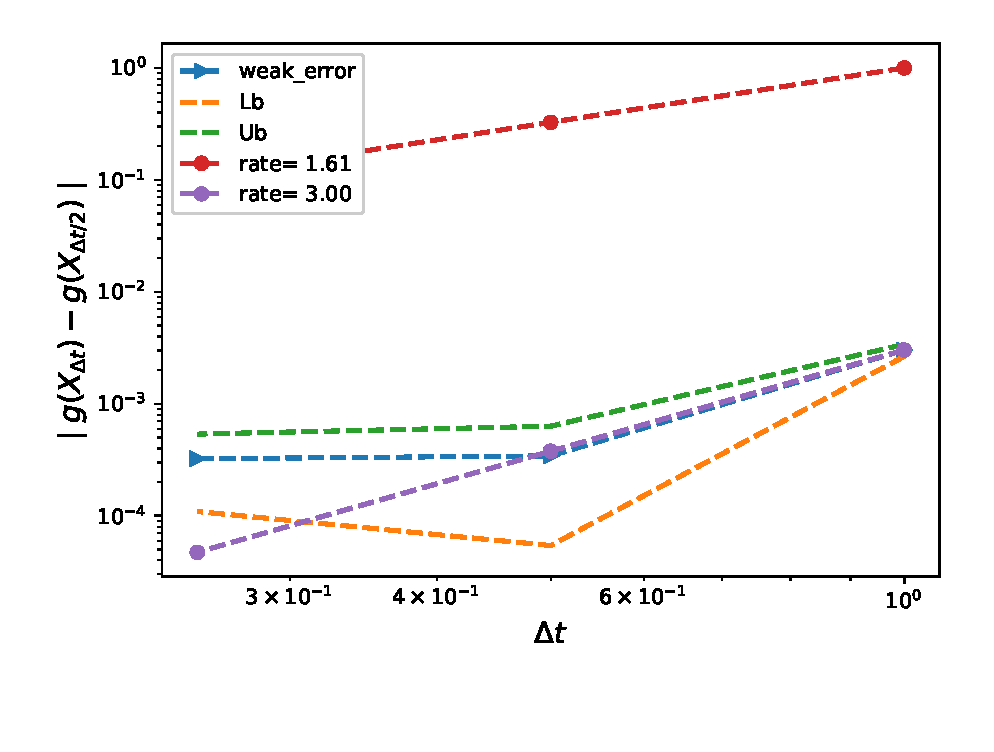
\includegraphics[width=1\linewidth]{./figures/weak_error_rates_call/Beta_32/with_rich/weak_convergence_order_differences_Call_richardson_level2_relative_M_5_10_6}
%		\caption{}
%		\label{fig:sub4}
%	\end{subfigure}
%	
%	\caption{The rate of convergence of the weak error for the  call option with Richardson extraploation (level 2), using MC with $M=5.10^6$: a) $\abs{\frac{1}{3}\expt{8 g(X_{\Delta t/4}) -6g(X_{\Delta t/2}) +g(X_{\Delta t})}-g(X)}$  b) $\abs{\frac{1}{3}\expt{-8 g(X_{\Delta t/8}) +14g(X_{\Delta t/4})-7 (X_{\Delta t/2}) +g(X_{\Delta t})}}$}
%	\label{fig:Weak_rate_call_with_rich_level2_beta_32}
%\end{figure}

\FloatBarrier
%\subsubsection{Comparing relative errors}\label{sec:Comparing relative errors, call}
%\subsubsection*{Without Richardson extrapolation}


%
%In this Section, we report the results for the Call option, using the different Methods: MISC, MC $+$ root finding  and MC, without Richardson extrapolation . We mention that for MISC we used a very small tolerance for the Newton solver, when solving the Kink point problem ($TOL_{\text{Newton}}=10^{-10}$), we also used $\beta=32$ (number of Laguerre quadrature points ). We start by reporting the observed approximated values using different methods (See table \ref{table:Call option price of the different methods for different number of time steps, without Richardson extrapolation.}). The biased values for MC method were computed using the values of Bias, reported in table \ref{Bias and Statistical errors of MC  for computing Call option price  for different number of time steps, without Richardson extrapolation. The numbers between parentheses are the corresponding absolute errors.}. In table \ref{Quadrature error of MISC to compute Call option price of the different tolerances for different number of time steps, without Richardson extrapolation. The numbers between parentheses are the corresponding absolute errors.}, we report the behavior of quadrature error with respect to MISC tolerance. We precise that the quadrature error is computed by substracting the MISC approximated value from the biased MC value. We report in red the values where MISC becomes stable (see also figure \ref{fig:Quadrature_error_non_rich_Call}). Those values where used to compute the needed number of samples for MC (with and without root finding), to achieve similar magnitude  for statistical error. Later, in table \ref{Total error of MISC and MC to compute Call option price of the different tolerances for different number of time steps, without Richardson extrapolation. The numbers between parentheses are the corresponding absolute errors.}, we report the total relative error for all methods (Quadrature error + Bias for MISC and Statistical error + Bias for MC). We also report in table \ref{Comparsion of the computational time of  MC and MISC, used to compute Call option price  for different number of time steps, without Richardson extrapolation}, the computational time needed for all different methods.  We finally provide in figure \ref{fig:Complexity plot for MC and MISC , Call non rich}, the complexity rates for the different involved methods.

%\begin{table}[h!]
%	\centering
%	\begin{tabular}{l*{6}{c}r}
%		Method \textbackslash  Steps            & $2$ & $4$ & $8$ & $16$ &   \\
%		\hline
%		MISC ($TOL_{\text{MISC}}=5.10^{-1},\beta=32$)  & $16.184$ & $16.070$ & $15.998$ & $15.930$  \\
%		MISC ($TOL_{\text{MISC}}=10^{-1},\beta=32$)  & $16.184$ & $16.070$ & $15.996$ &$15.928$  \\
%		MISC ($TOL_{\text{MISC}}=5.10^{-2},\beta=32$) & $16.184$ & $16.070$ & $15.996$ & $15.928$  \\
%		MISC ($TOL_{\text{MISC}}=10^{-2},\beta=32$) & $16.184$ & $16.103$ & $15.996$ &$15.928$  \\
%%		MISC ($TOL_{\text{MISC}}=10^{-3},\beta=32$) & $16.184$ & $16.103$ & $15.996$ & $-$  \\
%		
%		\hline
%		MC method ($M=10^{5}$)   & $  16.194$ & $ 16.099$ & $
%		15.999$ & $  15.923$  \\
%		\hline
%	\end{tabular}
%	\caption{Call option price of the different methods for different number of time steps, without Richardson extrapolation.}
%	\label{table:Call option price of the different methods for different number of time steps, without Richardson extrapolation.}
%\end{table}

%
%\begin{table}[h!]
%	\centering
%	\begin{tabular}{l*{6}{c}r}
%		Method \textbackslash  Steps            & $2$ & $4$ & $8$ & $16$  \\
%		\hline
%		MC Bias ($M=10^{5}$)  & 	$ \underset{(      0.3424 )}{\mathbf{0.0216}}$  & $\underset{(0.2473)}{\mathbf{ 0.0156
%		}}$  & $\underset{(  0.1474)}{\mathbf{0.0093}}$ & $\underset{(     0.0713
%	)}{\mathbf{  0.0045 }}$\\ 
%		
%		MC Statistical error  ($M=10^{5}$)   & 	$ \underset{( 7.5e-03  )}{\mathbf{4.4e-04}}$  & $\underset{(7.5e-03 )}{\mathbf{ 4.7e-04
%		}}$  & $\underset{(6.3e-03 )}{\mathbf{4.0e-04}}$ & $\underset{( 4.9e-03 )}{\mathbf{ 3.1e-04  }}$\\ 
%	
%%		MC Statistical error ($M=10^4$)     & 	$ \underset{( 2.2e-02  )}{\mathbf{1.4e-03}}$  & 	$ \underset{( 2.2e-02  )}{\mathbf{1.4e-03}}$  & $\underset{(1.9e-02 )}{\mathbf{1.2e-03}}$ & $\underset{( 1.5e-02 )}{\mathbf{ 9.3e-04  }}$\\ 
%%		
%		\hline
%	\end{tabular}
%	\caption{Bias and statistical errors of MC  for computing call option price  for different number of time steps, without Richardson extrapolation. The numbers between parentheses are the corresponding absolute errors.}
%	\label{Bias and Statistical errors of MC  for computing Call option price  for different number of time steps, without Richardson extrapolation. The numbers between parentheses are the corresponding absolute errors.}
%\end{table}



%
%\begin{table}[h!]
%	\centering
%	\begin{tabular}{l*{6}{c}r}
%		Method \textbackslash  Steps            & $2$ & $4$ & $8$ & $16$  \\
%		\hline
%		MISC ($TOL_{\text{MISC}}=5.10^{-1}$)  & $\underset{( 0.0103)}{\mathbf{\red{0.0007}}}$ & $\underset{(0.0290)}{\mathbf{0.0018}}$  & $\underset{(0.0010
%			)}{\mathbf{6.3e-05}}$ &$\underset{(   0.0070)}{\mathbf{0.0004}}$ \\
%		MISC ($TOL_{\text{MISC}}=10^{-1}$)   &  $\underset{( 0.0103)}{\mathbf{0.0007}}$& $\underset{(0.0290)}{\mathbf{0.0018}}$ & $\underset{(
%			0.0030
%			)}{\mathbf{\red{0.0002}}}$ &$\underset{(0.0020)}{\mathbf{\red{0.0001}}}$ \\
%		MISC ($TOL_{\text{MISC}}=5.10^{-2}$)  &$\underset{( 0.0103)}{\mathbf{0.0007}}$ & $\underset{(0.0290)}{\mathbf{0.0018}}$  & $\underset{(
%			0.0030
%			)}{\mathbf{0.0002}}$ &$\underset{(0.0020)}{\mathbf{0.0001}}$ \\
%		MISC ($TOL_{\text{MISC}}=10^{-2}$)  & $\underset{( 0.0103)}{\mathbf{0.0007}}$ & $\underset{( 0.0040)}{\mathbf{\red{0.0003}}}$  & $\underset{(
%			0.0030
%			)}{\mathbf{0.0002}}$ &$\underset{(0.0020)}{\mathbf{0.0001}}$ \\
%%		MISC ($TOL_{\text{MISC}}=10^{-3}$)  & $\underset{( 0.0103)}{\mathbf{0.0007}}$  & $\underset{( 0.0040)}{\mathbf{0.0003}}$ & $\underset{(
%%			0.0030
%%			)}{\mathbf{0.0002}}$ &$\underset{(-)}{\mathbf{-}}$ \\
%%		
%		\hline
%	\end{tabular}
%	\caption{Quadrature error of MISC, with different tolerances, to compute call option price for different number of time steps, without Richardson extrapolation. The numbers between parentheses are the corresponding absolute errors. The values marked in red correspond to stable quadrature errors for MISC, and will be used for complexity comparison against MC.}
%	\label{Quadrature error of MISC to compute Call option price of the different tolerances for different number of time steps, without Richardson extrapolation. The numbers between parentheses are the corresponding absolute errors.}
%\end{table}
%
%\FloatBarrier
%	\begin{figure}[h!]
%\centering
%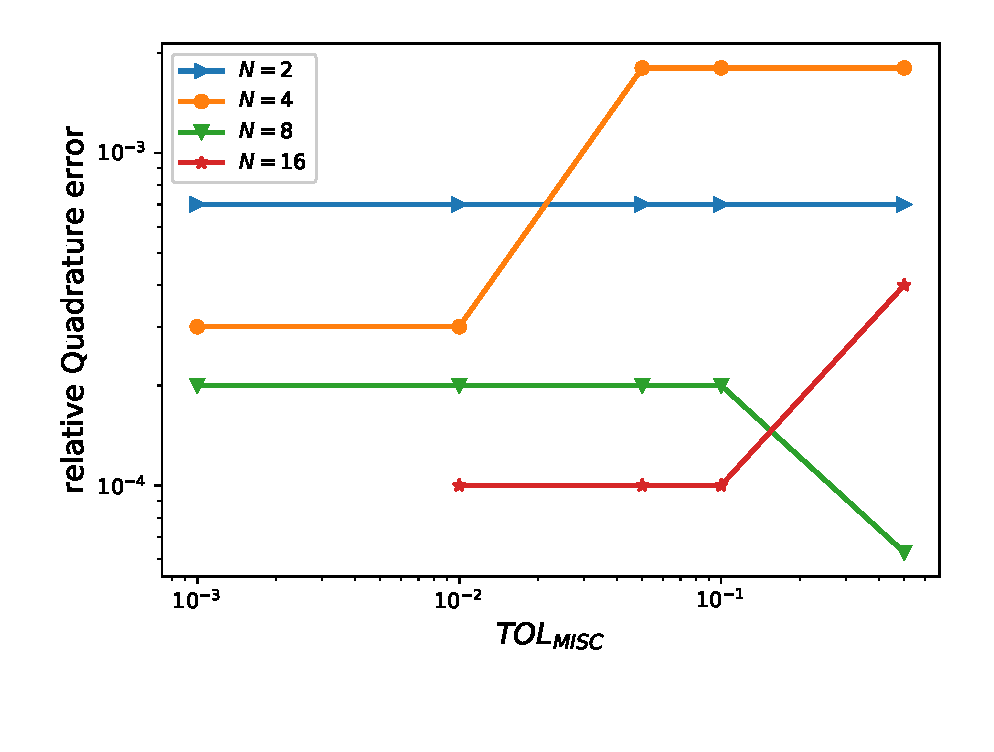
\includegraphics[width=0.4\linewidth]{./figures/Call_MISC_quadrature_error/relative_quad_error_wrt_MISC_TOL_non_rich}
%
%
%\caption{Relative quadrature error of MISC, with different tolerances, to compute call option price for different number of time steps, without Richardson extrapolation.}
%\label{fig:Quadrature_error_non_rich_Call}
%\end{figure}
%

\FloatBarrier
\begin{table}[h!]
	\centering
	\begin{tabular}{l*{6}{c}r}
		\toprule[1.5pt]
	Method & & Steps  & &     \\
	\hline
           & $2$ & $4$ & $8$ & $16$  \\
		\hline
%		($TOL_{\text{MISC}}=5.10^{-1}$, $\beta=32$)  
		ASGQ &  $\underset{(0.021,0.001)}{\mathbf{0.022}}$ & $\underset{(0.016,0.002)}{\mathbf{0.018}}$ & $\underset{(0.009,0.0001)}{\mathbf{0.009}}$ & $\underset{(0.004,0.0004)}{\mathbf{0.004}}$  \\
%		MISC ($TOL_{\text{MISC}}=10^{-1}$)  &  $\underset{(0.022,0.001)}{\mathbf{0.023}}$& $\underset{(0.016,0.002)}{\mathbf{0.018}}$ & $\underset{(0.009,0.0002)}{\mathbf{\red{0.009}}}$ & $\underset{(0.005,0.0001)}{\mathbf{\red{0.005}}}$  \\
%		MISC ($TOL_{\text{MISC}}=5.10^{-2}$) & $\underset{(0.022,0.001)}{\mathbf{0.0223}}$ & $\underset{(0.016,0.002)}{\mathbf{0.018}}$ &  $\underset{(0.009,0.0002)}{\mathbf{0.009}}$ & $\underset{(0.005,0.0001)}{\mathbf{0.005}}$  \\
%		MISC ($TOL_{\text{MISC}}=10^{-2}$)  &  $\underset{(0.022,0.001)}{\mathbf{0.023}}$& $\underset{(0.016,0.0003)}{\mathbf{\red{0.016}}}$ & $\underset{(0.009,0.0002)}{\mathbf{0.009}}$ &  $\underset{(0.005,0.0001)}{\mathbf{0.005}}$  \\
%		MISC ($TOL_{\text{MISC}}=10^{-3}$) &  $\mathbf{0.0223}$ & $\mathbf{0.0159}$ & $\mathbf{0.0095}$ & $\mathbf{}$  \\
		
		\hline
%		MC  ($M=10^5$)   &  $\mathbf{0.0266}$ & $\mathbf{0.0161}$ & $\mathbf{0.0097}$ & $\mathbf{\red{0.0048}}$  \\	
%		($\beta=32$) 
			MC +root finding  &  $\underset{(0.021,0.02)}{\mathbf{0.041}}$ & $\underset{(0.016,0.016)}{\mathbf{0.032}}$ & $\underset{(0.009,0.009)}{\mathbf{0.018}}$ & $\underset{(0.004,0.004)}{\mathbf{0.008}}$  \\
			M(\# MC samples)   & $10^2 $  & $3 \times 10^2 $  & $
			10^3$ & $4 \times 10^3$ \\	
		\hline	
				MC   &  $\underset{(0.02,0.02)}{\mathbf{0.04}}$ & $\underset{(0.016,0.016)}{\mathbf{0.032}}$ & $\underset{(0.01,0.01)}{\mathbf{}0.02}$ & $\underset{(0.004,0.004)}{\mathbf{0.008}}$  \\	
				M(\# MC samples)   & $3 \times 10^4$  & $5\times 10^4$  & $2\times 10^5$ & $8\times 10^5$ \\	
		
			\bottomrule[1.25pt]
	\end{tabular}
	\caption{Total relative  error of ASGQ, with different tolerances, and MC to compute call option price for different number of time steps, without Richardson extrapolation. The values between parentheses correspond to the different errors contributing to the total relative error: for ASGQ we report the bias and quadrature errors and for MC we report the bias and the statistical errors. The number of MC samples,$ M$, is chosen to satisfy \eqref{optimal_number_samples}.}
	\label{Total error of MISC and MC to compute Call option price of the different tolerances for different number of time steps, without Richardson extrapolation. The numbers between parentheses are the corresponding absolute errors.}
\end{table}

\FloatBarrier




\begin{table}[h!]
	\centering
	\begin{tabular}{l*{6}{c}r}
		\toprule[1.5pt]
	Method & & Steps  & &     \\
	\hline
	         & $2$ & $4$ & $8$ & $16$ &   \\
		\hline
%		($TOL_{\text{MISC}}=5.10^{-1}$, $\beta=32$)
		ASGQ  & $0.3$ & $3$ & $17$ & $473$  \\
%		MISC ($TOL_{\text{MISC}}=10^{-1}$)  & $0.3$ & $3$ & $\red{58}$ & $\red{656}$  \\
%		MISC ($TOL_{\text{MISC}}=5.10^{-2}$)   & $0.3$ & $3$ & $73$ & $731$  \\
%		MISC ($TOL_{\text{MISC}}=10^{-2}$)  & $0.3$ & $\red{6}$ & $108$ & $1972$  \\
%%		MISC ($TOL_{\text{MISC}}=10^{-3}$)   & $0.3$ & $28$ & $264$ & $-$  \\
%		\hline
%		MC method ($M=10^5, \beta=32$)    & $168$ & $216$ & $290$ & $\red{432}$  \\
%($\beta=32$) 
			MC +root finding  & $3$ & $16$ & $70$ & $408$  \\
				MC  & $3$ & $13$ & $76$ & $380$  \\
%		\hline
%		
%			Ratio of	$\text{(MC+root finding)}/\text{(MISC)}$ & $\red{ 4400}$ & $\red{   1400}$ & $\red{369}$ & $\red{ 107}$  \\
%		Ratio of	$(\text{MC})/(\text{MISC})$ & $\red{ 4800}$ & $\red{ 1665}$ & $\red{ 565}$ & $\red{ 241}$  \\
		\bottomrule[1.25pt]
	\end{tabular}
	\caption{Comparison of the computational time of  MC and ASGQ, used to compute call option price  for different number of time steps, without Richardson extrapolation. The average computational time of MC is computed over $10$ runs.}
	\label{Comparsion of the computational time of  MC and MISC, used to compute Call option price  for different number of time steps, without Richardson extrapolation}
\end{table}



\FloatBarrier
	\begin{figure}[h!]
\centering
\includegraphics[width=0.4\linewidth]{./figures/Call_Complexity_rates/error_vs_time}

\caption{Computational work comparison for ASGQ and MC methods, for the case of  call option. This plot shows that to achieve a relative error below $1\%$, ASGQ outperforms significantly MC method in terms of computational time.}
\label{fig:Complexity plot for MC and MISC , Call non rich}
\end{figure}


\FloatBarrier

%\subsubsection*{With Richardson extrapolation (level $1$)}
%
%
%
%%%
%%%In this Section, we report the results for the Call option, using the different Methods: MISC, MC $+$ root finding  and MC, with Richardson extrapolation . We mention that for MISC we used a very small tolerance for the Newton solver, when solving the Kink point problem ($TOL_{\text{Newton}}=10^{-10}$), we also used $\beta=32$ (number of Laguerre quadrature points ). We start by reporting the observed approximated values using different methods (See table \ref{table: Call option price of the different methods for different number of time steps, with Richardson extrapolation (level1).}. The biased values for MC method were computed using the values of Bias, reported in table \ref{Bias and Statistical errors of MC  for computing Call option price  for different number of time steps, with Richardson extrapolation (level $1$). The numbers between parentheses are the corresponding absolute errors.}. In table \ref{Quadrature error of MISC to compute Call option price of the different tolerances for different number of time steps, with Richardson extrapolation (level $1$). The numbers between parentheses are the corresponding absolute errors.}, we report the behavior of quadrature error with respect to MISC tolerance. We precise that the quadrature error is computed by substracting the MISC approximated value from the biased MC value. We report in red the values where MISC becomes stable (see also figure \ref{fig:Quadrature_error_with_rich_Call}). Those values where used to compute the needed number of samples for MC (with and without root finding), to achieve similar magnitude  for statistical error. Later, in table \ref{Total error of MISC and MC to compute Call option price of the different tolerances for different number of time steps, with Richardson extrapolation (level $1$). The numbers between parentheses are the corresponding absolute errors.}, we report the total relative error for all methods (Quadrature error + Bias for MISC and Statistical error + Bias for MC). We also report in table\ref{Comparsion of the computational time of  MC and MISC, used to compute Call option price  for different number of time steps, with Richardson extrapolation (level $1$)}, the computational time needed for all different methods.  We finally provide in figure \ref{fig:Complexity plot for MC and MISC , Call, comparison}, the comparison between the two versions of MISC (without/with Richardson extrapolation).
%
%
%%
%%\begin{table}[h!]
%%	\centering
%%	\begin{tabular}{l*{6}{c}r}
%%		Method \textbackslash  Steps            & $1-2$ & $2-4$ & $4-8$ & $8-16$ &   \\
%%		\hline
%%		MISC ($TOL_{\text{MISC}}=5.10^{-1}$)  & $16.4108$ & $16.0254$ & $15.8912$ & $15.8621$  \\
%%		MISC ($TOL_{\text{MISC}}=10^{-1}$)  & $16.4108$ & $16.0254$ & $15.8883$ & $15.8603$  \\
%%		MISC ($TOL_{\text{MISC}}=5.10^{-2}$) & $16.4108$ & $16.0218$ & $15.8885$ & $15.8600$  \\
%%%		MISC ($TOL_{\text{MISC}}=10^{-2}$) & $16.4108$& $16.0218$ & $15.8888$ & $15.8595$  \\
%%%		MISC ($TOL_{\text{MISC}}=10^{-3}$) & $16.4108$ & $16.0207$ & $15.8885$ & $-$  \\
%%		
%%		\hline
%%		MC method ($M=5.10^{6}$)   & $  16.4147$ & $ 16.0184$ & $15.8900$ & $15.8567$  \\
%%		\hline
%%	\end{tabular}
%%	\caption{Call option price of the different methods for different number of time steps, with Richardson extrapolation (level $1$).}
%%	\label{table: Call option price of the different methods for different number of time steps, with Richardson extrapolation (level1).}
%%\end{table}
%
%%
%%\begin{table}[h!]
%%	\centering
%%	\begin{tabular}{l*{6}{c}r}
%%		Method \textbackslash  Steps            & $1-2$ & $2-4$ & $4-8$ & $8-16$  \\
%%		\hline
%%		MC Bias ($M=5.10^6$)   & 	$ \underset{(    0.5627
%%			 )}{\mathbf{0.0355}}$  & $\underset{(  0.1664)}{\mathbf{ 0.0105
%%		}}$  & $\underset{( 0.0380)}{\mathbf{0.0024}}$ & $\underset{( 0.0048
%%	 )}{\mathbf{ 0.0003  }}$\\ 
%%		
%%		MC Statistical error ($M=5.10^6$)     & 	$ \underset{(  4.4e-03 )}{\mathbf{2.8e-04}}$  & $\underset{(3.8e-03 )}{\mathbf{ 2.4e-04
%%		}}$  & $\underset{(3.0e-03)}{\mathbf{1.9e-04}}$ & $\underset{(2.2e-03 )}{\mathbf{ 1.4e-04  }}$\\ 
%%		
%%%			MC Statistical error ($M=10^5$)     & 	$ \underset{(  1.4e-02 )}{\mathbf{9.0e-04}}$  & $\underset{(1.3e-02)}{\mathbf{ 8.0e-04
%%%		}}$  & $\underset{(9.4e-03)}{\mathbf{5.9e-04}}$ & $\underset{( 7.1e-03 )}{\mathbf{ 4.5e-04  }}$\\ 
%%		\hline
%%	\end{tabular}
%%	\caption{Bias and statistical errors of MC  for computing Call option price  for different number of time steps, with Richardson extrapolation (level $1$). The numbers between parentheses are the corresponding absolute errors.}
%%	\label{Bias and Statistical errors of MC  for computing Call option price  for different number of time steps, with Richardson extrapolation (level $1$). The numbers between parentheses are the corresponding absolute errors.}
%%\end{table}
%
%
%
%%
%%\begin{table}[h!]
%%	\centering
%%	\begin{tabular}{l*{6}{c}r}
%%		Method \textbackslash  Steps            & $1-2$ & $2-4$ & $4-8$ & $8-16$  \\
%%		\hline
%%		MISC ($TOL_{\text{MISC}}=5.10^{-1}$)  & $\underset{(0.0039
%%			)}{\mathbf{ \red{2.5e-04}}}$ & $\underset{(0.0070)}{\mathbf{4.4e-04}}$  & $\underset{(0.0012
%%			)}{\mathbf{7.6e-05}}$ &$\underset{(0.0054)}{\mathbf{3.4e-04}}$ \\
%%		MISC ($TOL_{\text{MISC}}=10^{-1}$)   & $\underset{(0.0039
%%			)}{\mathbf{ 2.5e-04}}$ & $\underset{(0.0070)}{\mathbf{4.4e-04}}$  & $\underset{(  0.0017)}{\mathbf{1.1e-04}}$ &$\underset{(0.0036)}{\mathbf{\red{2.3e-04}}}$ \\
%%		MISC ($TOL_{\text{MISC}}=5.10^{-2}$)  & $\underset{(0.0039
%%			)}{\mathbf{ 2.5e-04}}$ & $\underset{(0.0034)}{\mathbf{\red{\red{2.1e-04}}}}$  & $\underset{(    0.0015)}{\mathbf{\red{9.5e-05}}}$ &$\underset{(0.0033)}{\mathbf{2.1e-04}}$ \\
%%%		MISC ($TOL_{\text{MISC}}=10^{-2}$)  & $\underset{(0.0039
%%%			)}{\mathbf{ 2.5e-04}}$ & $\underset{(0.0034)}{\mathbf{2.1e-04}}$  & $\underset{(0.0012
%%%			)}{\mathbf{7.6e-05}}$&$\underset{(0.0028
%%%			)}{\mathbf{1.7e-04}}$ \\
%%%		MISC ($TOL_{\text{MISC}}=10^{-3}$)  & $\underset{(0.0039
%%%			)}{\mathbf{ 2.5e-04}}$ & $\underset{(0.0023
%%%			)}{\mathbf{1.5e-04}}$   &$\underset{(    0.0015)}{\mathbf{9.5e-05}}$ & $\underset{()}{\mathbf{}}$ \\
%%		
%%		\hline
%%	\end{tabular}
%%	\caption{Quadrature error of MISC, with different tolerances, to compute call option price  for different number of time steps, with Richardson extrapolation (level $1$). The numbers between parentheses are the corresponding absolute errors. The values marked in red correspond to stable quadrature errors for MISC, and will be used for complexity comparison against MC.}
%%	\label{Quadrature error of MISC to compute Call option price of the different tolerances for different number of time steps, with Richardson extrapolation (level $1$). The numbers between parentheses are the corresponding absolute errors.}
%%\end{table}
%
%%\FloatBarrier
%%
%%
%%	\begin{figure}[h!]
%%\centering
%%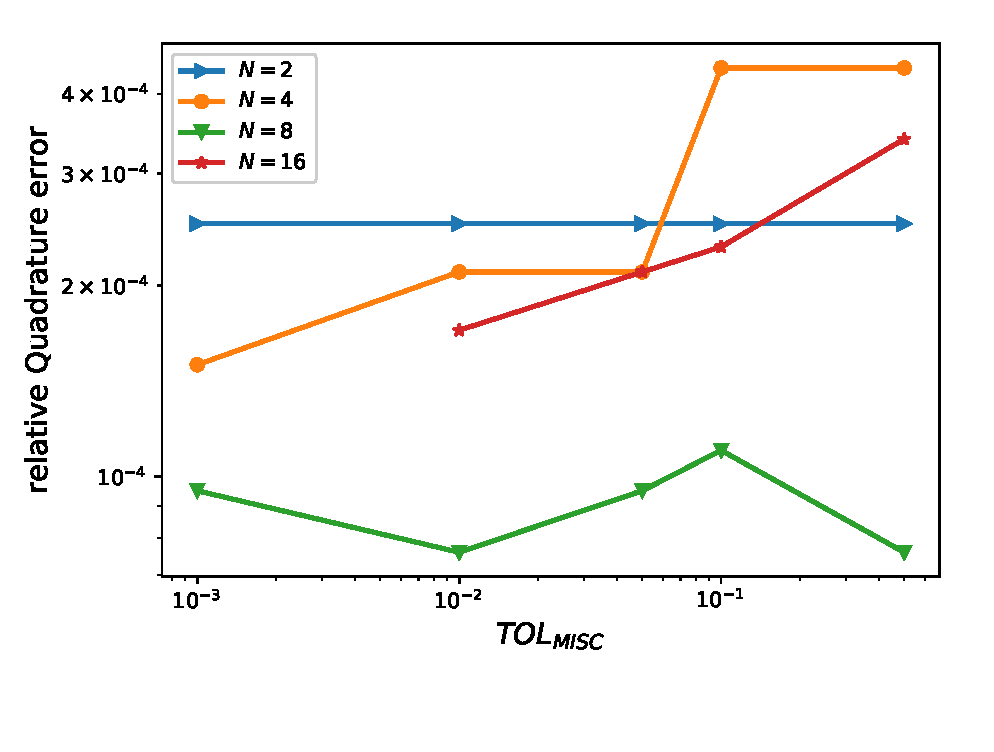
\includegraphics[width=0.4\linewidth]{./figures/Call_MISC_quadrature_error/relative_quad_error_wrt_MISC_TOL_with_rich}
%%
%%
%%\caption{Relative quadrature error of MISC, with different tolerances, to compute call option price for different number of time steps, with Richardson extrapolation.}
%%\label{fig:Quadrature_error_with_rich_Call}
%%\end{figure}
%%
%
%
%
%\FloatBarrier
%
%\begin{table}[h!]
%	\centering
%	\begin{tabular}{l*{6}{c}r}
%		\toprule[1.5pt]
%	Method & & Steps  &  &   \\
%	\hline
%	           & $1-2$ & $2-4$ & $4-8$ & $8-16$  \\
%		\hline
%		MISC ($TOL_{\text{MISC}}=5.10^{-1}$)  &  $\underset{(0.036,0.0003)}{\mathbf{0.036}}$ & $\underset{(0.011,0.0004)}{\mathbf{0.011}}$ & $\underset{(0.002,0.0001)}{\mathbf{0.002}}$ & $\underset{(0.0003,0.0003)}{\mathbf{0.0006}}$  \\
%%		MISC ($TOL_{\text{MISC}}=10^{-1}$)  &  $\underset{(0.036,0.0003)}{\mathbf{0.036}}$ & $\underset{(0.011,0.0004)}{\mathbf{0.011}}$ & $\underset{(0.002,0.0001)}{\mathbf{0.002}}$ & $\underset{(0.0003,0.0002)}{\mathbf{\red{0.0005}}}$  \\
%%		MISC ($TOL_{\text{MISC}}=5.10^{-2}$) &  $\underset{(0.036,0.0003)}{\mathbf{0.036}}$ & $\underset{(0.011,0.0002)}{\mathbf{\red{0.011}}}$ & $\underset{(0.002,0.0001)}{\mathbf{\red{0.002}}}$ & $\underset{(0.0003,0.0002)}{\mathbf{0.0005}}$  \\
%%		MISC ($TOL_{\text{MISC}}=10^{-2}$)  &  $\mathbf{0.0358}$ & $\mathbf{0.0107}$ & $\mathbf{0.0025}$ & $\mathbf{0.0005}$ \\
%%		MISC ($TOL_{\text{MISC}}=10^{-3}$) &  $\mathbf{0.0358}$ & $\mathbf{0.0107}$ & $\mathbf{0.0025}$ & $\mathbf{}$  \\
%		
%%		\hline
%%		MC  ($M=5.10^6$)   &  $\mathbf{\red{0.0358}}$ & $\mathbf{\red{0.0107}}$ & $\mathbf{\red{0.0026}}$ & $\mathbf{\red{0.0004}}$  \\	
%%			MC + root finding  &  $\mathbf{\red{0.0358}}$ & $\mathbf{\red{0.0107}}$ & $\mathbf{\red{0.0025}}$ & $\mathbf{\red{0.}}$  \\	
%		\bottomrule[1.25pt]
%	\end{tabular}
%	\caption{Total relative error of MISC, with different tolerances,  to compute call option price for different number of time steps, with Richardson extrapolation (level $1$).  The values marked in red, for MISC method, correspond to the total relative errors associated with  stable quadrature errors for MISC, and will be used for complexity comparison against MC.}
%	\label{Total error of MISC and MC to compute Call option price of the different tolerances for different number of time steps, with Richardson extrapolation (level $1$). The numbers between parentheses are the corresponding absolute errors.}
%\end{table}
%
%
%
%\FloatBarrier
%
%
%\begin{table}[h!]
%	\centering
%	\begin{tabular}{l*{6}{c}r}
%		\toprule[1.5pt]
%	Method & & Steps  &  &   \\
%	\hline
%         & $1-2$ & $2-4$ & $4-8$ & $8-16$ &   \\
%		\hline
%		MISC ($TOL_{\text{MISC}}=5.10^{-1}$) & $0.3$ & $4$ & $56$ & $713$  \\
%%		MISC ($TOL_{\text{MISC}}=10^{-1}$)  & $0.3$  & $4$ & $107$ & $\red{1126}$  \\
%%		MISC ($TOL_{\text{MISC}}=5.10^{-2}$)   & $0.3$  & $\red{9}$ & $\red{135}$ & $1253$  \\
%%%		MISC ($TOL_{\text{MISC}}=10^{-2}$)  &  $0.3$  & $9$ & $186$ & $3540$  \\
%%%		MISC ($TOL_{\text{MISC}}=10^{-3}$)   & $0.3$  & $63$ & $836$ & $$  \\
%%		\hline
%%		MC +root finding   & $\red{ 2.4e+05}$ & $\red{ 4.3e+05}$ & $\red{ 3.5e+06}$ & $\red{-}$  \\
%	\bottomrule[1.25pt]
%	\end{tabular}
%	\caption{Comparison of the computational time of  MISC, used to compute call option price  for different number of time steps, with Richardson extrapolation (level $1$). The average computational time of MC is computed over $10$ runs.}
%	\label{Comparsion of the computational time of  MC and MISC, used to compute Call option price  for different number of time steps, with Richardson extrapolation (level $1$)}
%\end{table}
%
%%	\begin{figure}[h!]
%%	\centering
%%	\includegraphics[width=0.7\linewidth]{./figures/Call_Complexity_rates/error_vs_time_rich}
%%	
%%	\caption{Complexity plot for MC and MISC for the case with Richardson extrapolation.}
%%	\label{fig:Complexity plot for MC and MISC , Call, with rich}
%%\end{figure}
%
%
%\FloatBarrier
%\begin{figure}[h!]
%	\centering
%	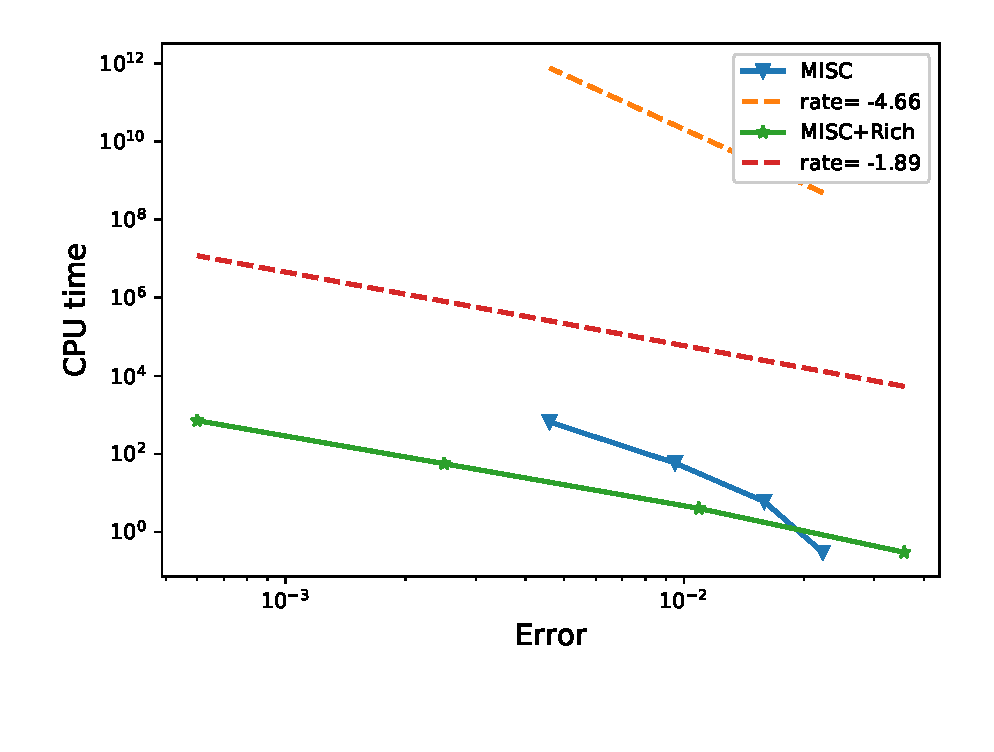
\includegraphics[width=0.4\linewidth]{./figures/Call_Complexity_rates/error_vs_time_comparision}
%	
%	\caption{Complexity plot for MISC without and with Richardson extrapolation, for the call option.}
%	\label{fig:Complexity plot for MC and MISC , Call, comparison}
%\end{figure}
%\FloatBarrier
%
%
%
%
%%In the following, we compare the  relative errors for the call option example under Black-Scholes model(see Tables (\ref{Relative error of the call option price of the different tolerances for different number of time steps.}, \ref{Relative error of Call option price of the different tolerances for different number of time steps, using Richardson extrapolation (level $1$)}, \ref{Relative error of Call option price of the different tolerances for different number of time steps, using Richardson extrapolation (level $2$)})). We report the results for $3$ scenarios: i) Without using Richardson extrapolation, ii) Using level $1$ Richardson extrapoaltion, iii) Using level $2$ Richardson extrapoaltion.  You may see appendix \ref{appendix:Call prices for different methods} for the values of call option prices. The value of $\beta$ used to get those points is $\beta=10$.
%%
%%Given the normalized bias computed by MC method (See Section \ref{sec:Weak error plots_call}) (reported as bold values in the tables), we report in red in each table the smallest tolerance that MISC required to get below that relative bias (I do not put values for smaller tolerances, once the required bias is reached). In case I do not reach those bias I put the best value that I get with MISC in red.
%%
%%From the tables (\ref{Relative error of the call option price of the different tolerances for different number of time steps.}, \ref{Relative error of Call option price of the different tolerances for different number of time steps, using Richardson extrapolation (level $1$)}, \ref{Relative error of Call option price of the different tolerances for different number of time steps, using Richardson extrapolation (level $2$)})), we may observe that to get a relative error below $0.5\%$, we need more than $16$ time steps for the case without Richardson extrapolation compared to only using $4$ time step in the coarse level for the case of level $1$ Richardson extraplation,  and  only using $1$ time step in the coarse level for the case of level $2$ Richardson extraplation.
%
%%\begin{table}[h!]
%%	\centering
%%	\begin{tabular}{l*{6}{c}r}
%%		Method \textbackslash  Steps            & $2$ & $4$ & $8$ & $16$ &   \\
%%		\hline
%%		MISC ($TOL_{\text{MISC}}=5.10^{-1}$)  & $ \red{0.0229}$ & $  0.0179$ & $\red{0.0111}$ & $ 0.0068$  \\
%%		MISC ($TOL_{\text{MISC}}=10^{-3}$)  & $-$ & $ \red{ 0.0177}$ & $-$ & $\red{  0.0066}$  \\
%%			MC method ($M=10^{5}$)&$ \mathbf{0.0231}$    & $\mathbf{0.0175}$  & $\mathbf{0.0111}$  & $\mathbf{0.0064}$ \\	
%%		\hline
%%	\end{tabular}
%%	\caption{Relative error of the call option price of the different tolerances for different number of time steps, without Richardson extrapolation}
%%	\label{Relative error of the call option price of the different tolerances for different number of time steps.}
%%\end{table}
%
%%\begin{table}[h!]
%%	\centering
%%	\begin{tabular}{l*{5}{c}r}
%%		Method \textbackslash  Steps    &$1-2$        & $2-4$ & $4-8$ & $8-16$  \\
%%		\hline
%%		MISC ($TOL_{\text{MISC}}=5.10^{-1}$)  &$\red{0.0372}$ & $ 0.0129$ & $0.0043$ & $ 0.0025$  \\
%%		MISC ($TOL_{\text{MISC}}=10^{-3}$) & $-$ & $ \red{0.0126}$ & $\red{    0.0042}$ & $\red{0.0023}$   \\
%%		MC method ($M=10^{5}$)&$ \mathbf{0.0374}$    & $\mathbf{0.0116}$  & $\mathbf{0.0027}$  & $\mathbf{0.0022}$ \\
%%		\hline
%%	\end{tabular}
%%	\caption{Relative error of the call option price of the different tolerances for different number of time steps, using Richardson extrapolation (level $1$)}
%%	\label{Relative error of Call option price of the different tolerances for different number of time steps, using Richardson extrapolation (level $1$)}
%%\end{table}
%
%
%%\begin{table}[h!]
%%	\centering
%%	\begin{tabular}{l*{5}{c}r}
%%		Method \textbackslash  Steps    &$1-2-4$        & $2-4-8$ & $4-8-16$   \\
%%		\hline
%%		MISC ($TOL_{\text{MISC}}=5.10^{-1}$)  &$0.0047$ & $  0.0015$ & $0.0019
%%		$   \\
%%		MISC ($TOL_{\text{MISC}}=10^{-3}$) & $ \red{0.0043}$ & $ \red{0.0013}$ & $\red{  0.0017}$    \\
%%		MC method ($M=10^{6}$)&$ \mathbf{0.0041}$    & $\mathbf{0.0013}$  & $\mathbf{0.0016}$  \\
%%		\hline
%%	\end{tabular}
%%	\caption{Relative error of the call option price of the different tolerances for different number of time steps, using Richardson extrapolation (level $2$)}
%%	\label{Relative error of Call option price of the different tolerances for different number of time steps, using Richardson extrapolation (level $2$)}
%%\end{table}
%
%


\subsection{The basket call option  under GBM  model}\label{sec:The basket call option  under GBM  model}
The third example that we consider  is the multi-dimensional  basket call option under GBM. 
\subsection{$d=2$}
For illustration, we start with the two dimensional basket call option  with parameters:  $S_0^{1,2}=K=100$, $\sigma_{1,2}=0.4$, $\rho=0.3$, $T=1$ $r=0$ and $c_{1,2}=1/2$, the reference value for those parameters  is  $12.90$. Figure \ref{fig:Weak_rate_two_dim_basket} shows the estimated   weak error  for the case without Richardson extrapolation, and we report the results for comparing MC and ASGQ in Tables \ref{Total error of MISC and MC to compute two  dim basket  Call option price of the different tolerances for different number of time steps, without Richardson extrapolation. The numbers between parentheses are the corresponding absolute errors.} and \ref{Comparsion of the computational time of  MC and MISC, used to compute two dim basket Call option price  for different number of time steps, without Richardson extrapolation}, and Figure \ref{fig:Complexity plot for MC and MISC , two dim basket call non rich}. Our numerical experiments show that ASGQ  requires approximately $5\%$ of the work of MC  to achieve a total relative error of around $0.9\%$.

\FloatBarrier
\begin{figure}[h!]
		\centering
		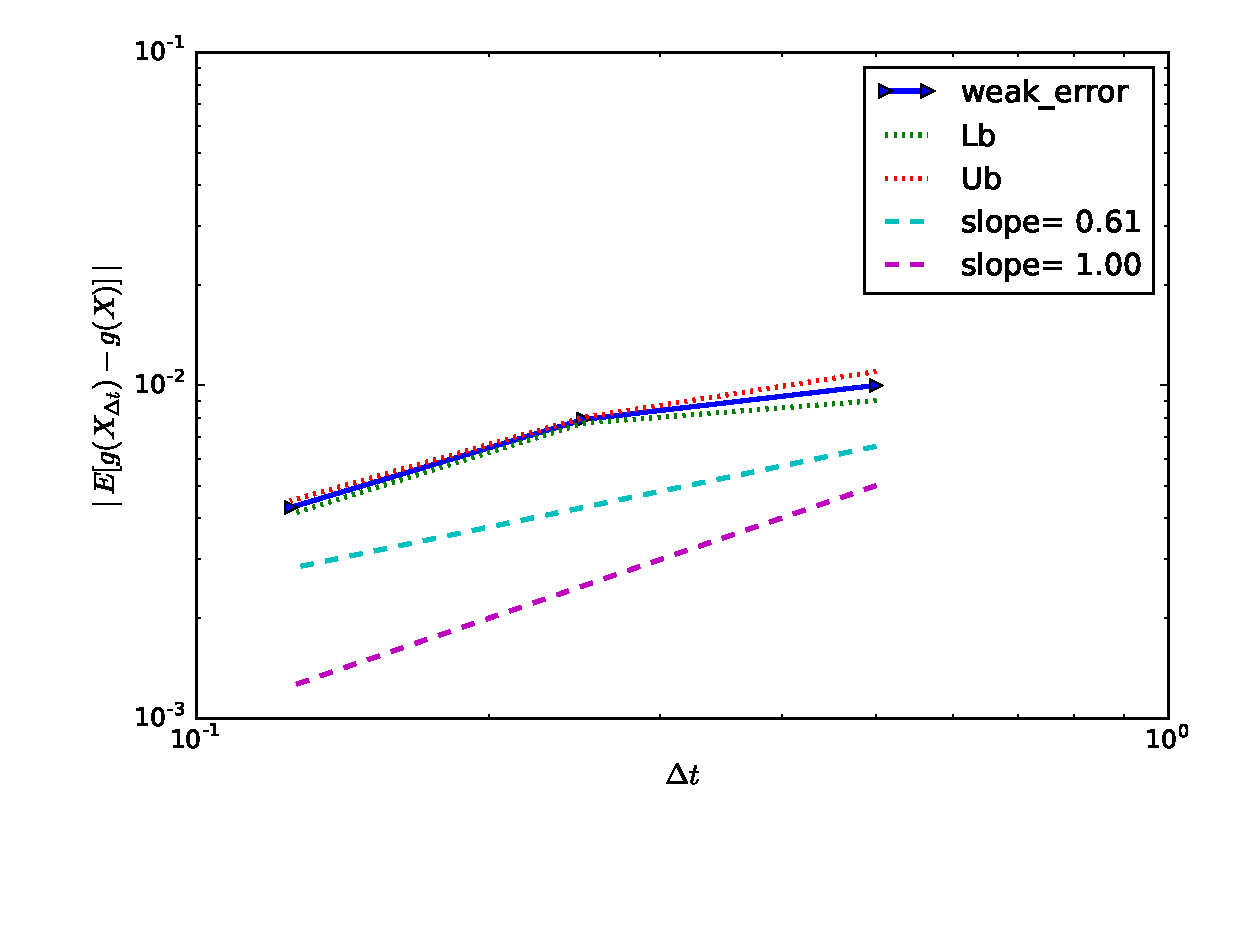
\includegraphics[width=0.4\linewidth]{./figures/basket_call_2d_time_stepping/weak_convergence/weak_convergence_order_basket_option_2d_relative_M_10_7_beta_128}

	\caption{The convergence of the relative weak error  $\mathcal{E}_B(N)$ defined in \ref{eq:total_error}, for the two dimensional basket call option with  a number of Laguerre  quadrature points  $\beta=128$ and number of samples for MC $M=10^7$. The upper and lower bounds are $95\%$ confidence intervals.}
	\label{fig:Weak_rate_two_dim_basket}
\end{figure}
\FloatBarrier


\FloatBarrier
\begin{table}[h!]
	\centering
	\begin{tabular}{l*{6}{c}r}
		\toprule[1.5pt]
	Method & & Steps  & &     \\
	\hline
           & $2$ & $4$ & $8$   \\
		\hline
		ASGQ   &  $\underset{(0.01,0.006)}{\mathbf{0.016}}$ & $\underset{(0.0079,0.0055)}{\mathbf{0.0134}}$ & $\underset{(0.0043,0.0042)}{\mathbf{0.0085}}$   \\

		\hline		
			MC +root finding   &  $\underset{(0.01,0.01)}{\mathbf{0.02}}$ & $\underset{(0.0079,0.0076)}{\mathbf{0.0155}}$ & $\underset{(0.0043,0.0038)}{\mathbf{0.0081}}$  \\
			M(\# MC samples)   & $2 \times 10^3$   &  $5 \times 10^3$ & $2 \times 10^4$  \\	
		\hline	
				MC   &  $\underset{(0.01,0.01)}{\mathbf{0.02}}$ & $\underset{(0.0079,0.0076)}{\mathbf{0.0155}}$ & $\underset{(0.0043,0.004)}{\mathbf{0.0083}}$   \\	
				M(\# MC samples)   &$10^5$  & $2 \times 10^5$  &  $8 \times 10^5$\\	
		
			\bottomrule[1.25pt]
	\end{tabular}
	\caption{Total relative  error of ASGQ, with different tolerances, and MC to compute two dimensional basket call option price for different number of time steps, without Richardson extrapolation. The values between parentheses correspond to the different errors contributing to the total relative error: for ASGQ we report the bias and quadrature errors and for MC we report the bias and the statistical errors. The number of MC samples,$ M$, is chosen to satisfy \eqref{optimal_number_samples}.}
	\label{Total error of MISC and MC to compute two  dim basket  Call option price of the different tolerances for different number of time steps, without Richardson extrapolation. The numbers between parentheses are the corresponding absolute errors.}
\end{table}
\FloatBarrier




\begin{table}[h!]
	\centering
	\begin{tabular}{l*{6}{c}r}
		\toprule[1.5pt]
	Method & & Steps  & &     \\
	\hline
	         & $2$ & $4$ & $8$    \\
		\hline
		ASGQ & $4$  & $8$ & $21$     \\
			MC +root finding  & $281$&  $814$&  $3888$   \\
				MC  &   $34$& $93$ &   $ 442$ \\
		\bottomrule[1.25pt]
	\end{tabular}
	\caption{Comparison of the computational time of  MC and ASGQ, used to compute two dimensional basket call option price  for different number of time steps, without Richardson extrapolation. The average computational time of MC is computed over $10$ runs.}
	\label{Comparsion of the computational time of  MC and MISC, used to compute two dim basket Call option price  for different number of time steps, without Richardson extrapolation}
\end{table}


\FloatBarrier
	\begin{figure}[h!]
\centering
\includegraphics[width=0.4\linewidth]{./figures/basket_call_2d_time_stepping/complexity_rates/error_vs_time}

\caption{Computational work comparison for ASGQ and MC methods, for the case of two dimensional basket call option. This plot shows that to achieve a relative error below $1\%$, ASGQ outperforms significantly MC method in terms of computational time.}
\label{fig:Complexity plot for MC and MISC , two dim basket call non rich}
\end{figure}


\FloatBarrier

\subsection{$d=4$}
We consider now  the four dimensional basket call option  with parameters:  $S_0^{1,2,3,4}=K=100$, $\sigma_{1,2,3,4}=0.4$, $\rho=0.3$, $T=1$ $r=0$ and $c_{1,2,3,4}=1/4$, the reference value for those parameters  is  $11.04$. Figure \ref{fig:Weak_rate_4_dim_basket} shows the estimated   weak error  for the case without Richardson extrapolation, and we report the results for comparing MC and ASGQ in Tables \ref{Total error of MISC and MC to compute 4 dim basket  Call option price of the different tolerances for different number of time steps, without Richardson extrapolation. The numbers between parentheses are the corresponding absolute errors.} and \ref{Comparsion of the computational time of  MC and MISC, used to compute 4 dim basket Call option price  for different number of time steps, without Richardson extrapolation}, and Figure \ref{fig:Complexity plot for MC and MISC , 4 dim basket call non rich}.  Our numerical experiments show that ASGQ  requires approximately $4\%$ of the work of MC  to achieve a total relative error of around $0.8\%$.

\FloatBarrier
\begin{figure}[h!]
		\centering
		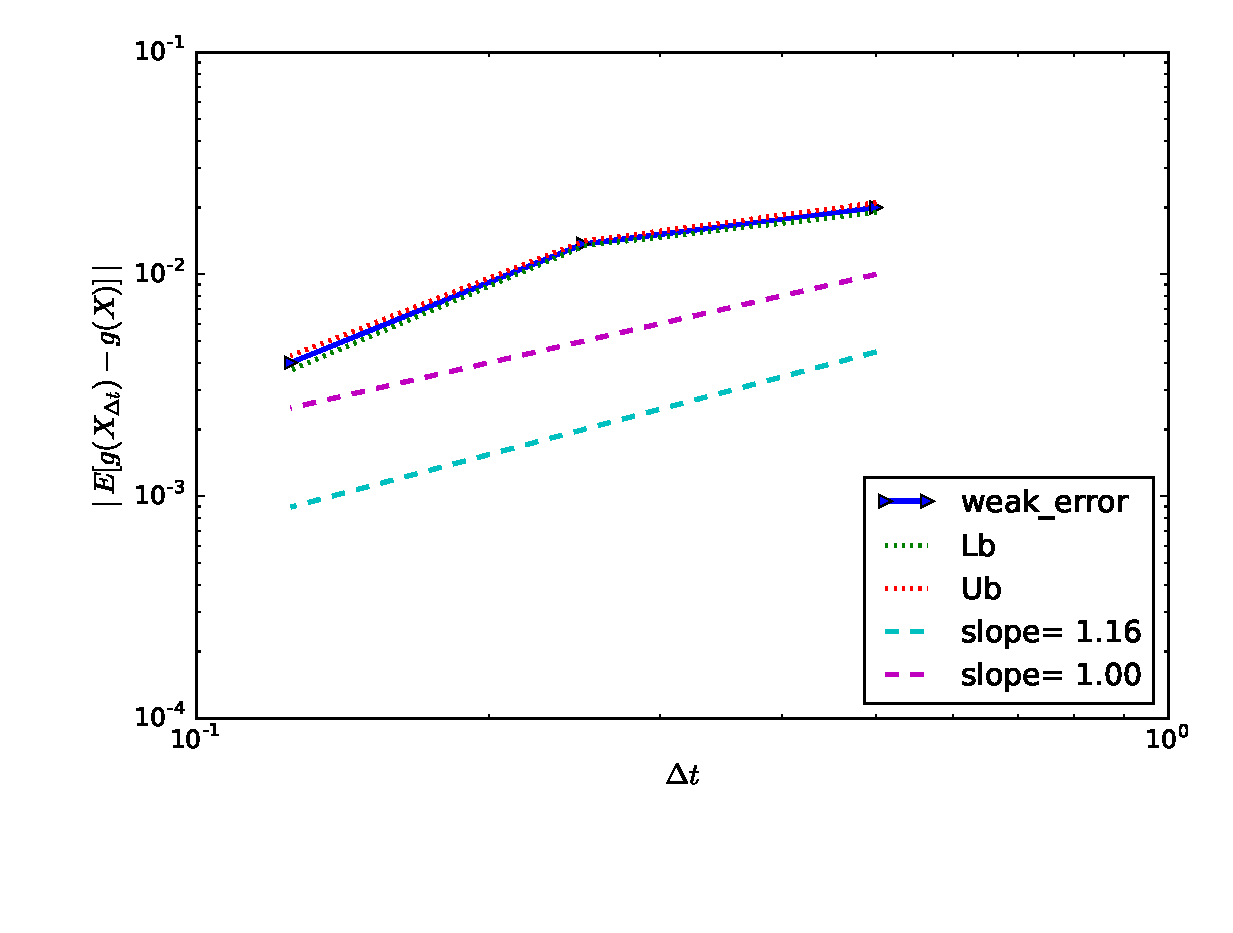
\includegraphics[width=0.4\linewidth]{./figures/basket_call_4d_time_stepping/weak_convergence/weak_convergence_order_basket_option_4d_relative_M_4_10_6_beta_256}

	\caption{The convergence of the relative weak error  $\mathcal{E}_B(N)$ defined in \ref{eq:total_error}, for the $4$-dimensional basket call option with  a number of Laguerre  quadrature points  $\beta=512$ and number of samples for MC $M=4 \times 10^6$. The upper and lower bounds are $95\%$ confidence intervals.}
	\label{fig:Weak_rate_4_dim_basket}
\end{figure}
\FloatBarrier

\FloatBarrier
\begin{table}[h!]
	\centering
	\begin{tabular}{l*{6}{c}r}
		\toprule[1.5pt]
	Method & & Steps  & &     \\
	\hline
           & $2$ & $4$ & $8$   \\
		\hline
		ASGQ   &  $\underset{(0.02,0.02)}{\mathbf{0.04}}$ & $\underset{(0.013,0.014)}{\mathbf{0.027}}$ & $\underset{(0.004,0.004)}{\mathbf{0.008}}$   \\

		\hline		
			MC +root finding   &  $\underset{(0.02,0.02)}{\mathbf{0.04}}$ & $\underset{(0.013,0.012)}{\mathbf{0.025}}$ & $\underset{(0.004,0.004)}{\mathbf{0.008}}$  \\
			M(\# MC samples)   & $10^3$   &  $3 \times 10^3$ &  $3 \times 10^4$  \\	
		\hline	
				MC   &  $\underset{(0.02,0.02)}{\mathbf{0.04}}$ & $\underset{(0.013,0.013)}{\mathbf{0.026}}$ & $\underset{(0.004,0.004)}{\mathbf{0.008}}$   \\	
				M(\# MC samples)   &$2 \times 10^4$  & $7 \times 10^4 $  &  $7 \times 10^5 $ \\	
		
			\bottomrule[1.25pt]
	\end{tabular}
	\caption{Total relative  error of ASGQ, with different tolerances, and MC to compute $4$-dimensional basket call option price for different number of time steps, without Richardson extrapolation. The values between parentheses correspond to the different errors contributing to the total relative error: for ASGQ we report the bias and quadrature errors and for MC we report the bias and the statistical errors. The number of MC samples,$ M$, is chosen to satisfy \eqref{optimal_number_samples}.}
	\label{Total error of MISC and MC to compute 4 dim basket  Call option price of the different tolerances for different number of time steps, without Richardson extrapolation. The numbers between parentheses are the corresponding absolute errors.}
\end{table}
\FloatBarrier




\begin{table}[h!]
	\centering
	\begin{tabular}{l*{6}{c}r}
		\toprule[1.5pt]
	Method & & Steps  & &     \\
	\hline
	         & $2$ & $4$ & $8$    \\
		\hline
		ASGQ & $4$  & $13$ & $22$     \\
			MC  +root finding  & $222$&  $730$&  $10541$   \\
				MC  &   $10$& $44$ &   $603$ \\
		\bottomrule[1.25pt]
	\end{tabular}
	\caption{Comparison of the computational time of  MC and ASGQ, used to compute $4$-dimensional basket call option price  for different number of time steps, without Richardson extrapolation. The average computational time of MC is computed over $10$ runs.}
	\label{Comparsion of the computational time of  MC and MISC, used to compute 4 dim basket Call option price  for different number of time steps, without Richardson extrapolation}
\end{table}


\FloatBarrier


	\begin{figure}[h!]
\centering
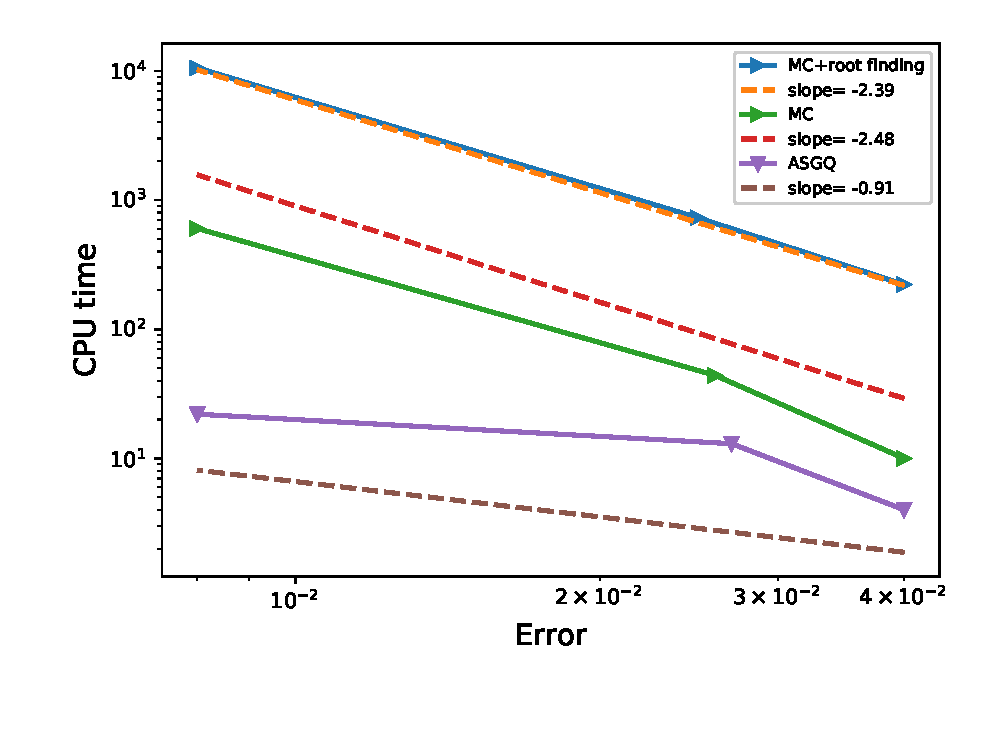
\includegraphics[width=0.4\linewidth]{./figures/basket_call_4d_time_stepping/complexity_rates/error_vs_time}

\caption{Computational work comparison for ASGQ and MC methods, for the case of $4$-dimensional basket call option. This plot shows that to achieve a relative error below $1\%$, ASGQ outperforms significantly MC method in terms of computational time.}
\label{fig:Complexity plot for MC and MISC , 4 dim basket call non rich}
\end{figure}


\FloatBarrier

%\subsection{The call on max  option under GBM}\label{sec:The best call option  under GBM}
%The fourth example that we consider is  the European rainbow option under BBM model and in particular the call on max option whose payoff is given by
%\begin{align}\label{eq:max_call_option}
%\max\left( \max\left(S_1,\dots,S_d\right)-K,0 \right).
%\end{align}
%
%We start here by the two dimensional call on max option under the GBM model. The discretization of the assets is the same as given in  \eqref{eq:discrete_rep_2} and \eqref{eq: incremental functions}, where we use the same transformation as in Section \ref{sec:Step $1$: Numerical smoothing}. This implies that, in order to determine $Y^{\ast}_1$, we need to solve
%\begin{align}
%	x=\max\left(X_0^{(1)}  \prod_{i=0}^{N-1} g_i^{(1)}(Y^{\ast}_1(x),\mathbf{Y}_{-1}),X_0^{(2)}  \prod_{i=0}^{N-1} g_i^{(2)}(Y^{\ast}_1(x),\mathbf{Y}_{-1})\right)
%\end{align}
%
%
%For illustration, we consider the example with parameters:  $S_0^{1,2}=K=100$, $\sigma_{1,2}=0.4$, $\rho=0.3$, $T=1$, and  $r=0$, the reference value for those parameters  is  $26.40$.




\subsection{Options under the discretized the Heston model}
In this section, we consider  testing options under the discretized Heston model \cite{heston1993closed,broadie2006exact,kahl2006fast,andersen2007efficient} whose dynamics are given by
\begin{align}\label{eq:dynamics Heston}
dS_t&=\mu S_t dt+\sqrt{v_t}S_t dW_t^S= \mu S_t dt+ \rho\sqrt{v_t}S_t dW_t^v+ \sqrt{1-\rho^2} \sqrt{v_t}S_t dW_t \nonumber\\
dv_t&=\kappa (\theta-v_t)dt+\xi \sqrt{v_t} dW_t^v\COMMA
\end{align}
where 

\begin{itemize}
\item $S_t$ is the price of the asset, $v_t$ the instantaneous variance, given as  a CIR process.
\item $W_{t}^{S},W_{t}^{v}$ are correlated Wiener processes with correlation $\rho$.
\item $\mu$  is the rate of return of the asset.
\item $\theta$ is  the mean  variance.
\item $\kappa$ is the rate at which $v_t$ reverts to $\theta$.
\item $\xi$ is the volatility of the volatility, and determines the variance of $v_t$.
\end{itemize}
%We also consider cases where the parameters fulfill the Feller condition
%\begin{align*}
%2 \kappa \theta >\xi^2,
%\end{align*}
%implying  that the process $v_t$ is strictly positive.

%\subsection{Schemes to simulate the Heston dynamics}\label{sec:Schemes to simulate the Heston dynamics}
Given that the SDE for the asset path is now dependent  upon the solution of the second volatility SDE in \eqref{eq:dynamics Heston}, it is necessary to simulate the volatility process first and then utilize this "volatility path" in order to simulate the asset path. In the case of the original GBM SDE it is possible to use It\^o's Lemma to directly solve for $S_t$. However, we are unable to utilize that procedure here and must use a numerical approximation in order to obtain both paths. In the following, we try to give an overview of the methods that we can use in our context. These methods mainly differs by the way it simulates the volatility process to ensure its positiveness.
\subsubsection{Fixed Euler scheme}\label{sec:Discretization of Heston model with a non smooth transformations for the volatility process}
In this context, one can use Forward Euler scheme to simulate the Heston model, and to avoid  problems with negative values of the volatility process $v_t$, many fixes  were introduced in the literature (see \cite{lord2010comparison}). We introduce $f_1, f_2$, and $f_3$, which with different choices implies different schemes, and   apply Forward Euler scheme to discretize \ref{eq:dynamics Heston}  results in
\begin{align}\label{eq:FE_Heston_discrete}
\hat{S}_{t+\Delta t}&= \hat{S}_t +\mu \hat{S}_t \Delta t+\sqrt{\hat{V}_t \Delta t} \hat{S}_t Z_s \nonumber\\
\hat{V}_{t+\Delta t}&=f_1(\hat{V}_t)+\kappa (\theta-f_2(\hat{V}_t)) \Delta t+\xi \sqrt{f_3(\hat{V}_t) \Delta t} Z_V \nonumber\\
\hat{V}_{t+\Delta t}&=f_3(\hat{V}_{t+\Delta t}) \COMMA
\end{align}
where $Z_s$ and $Z_V$  are two correlated standard normal variables with correlation $\rho$, such that $Z_s=\rho Z_V+\sqrt{1-\rho^2} Z_t$. 

\FloatBarrier
\begin{table}[h!]
	\centering
	\begin{tabular}{l*{6}{c}r}
		\toprule[1.5pt]
	Scheme &  $f_1$& $f_2$  & $f_3$     \\
	\hline
	full truncation scheme & $\hat{V}_t$ &  $\hat{V}_t^+$&$\hat{V}_t^+$\\
	Partial truncation scheme & $\hat{V}_t$ &  $\hat{V}_t$&$\hat{V}_t^+$\\
	The reflection scheme  &$\abs{\hat{V}_t}$ & $\abs{\hat{V}_t}$& $\abs{\hat{V}_t}$\\
			\bottomrule[1.25pt]
	\end{tabular}
	\label{Numerical schemes for CIR process}
\end{table}
\FloatBarrier
where  $\hat{V}_t^+=\max(0,\hat{V}_t)$.

\cite{lord2010comparison} suggest that the Full Truncation method is the optimal option in terms of weak error convergence and robustness with respect to the parameters of the model. Therefore,  we use this scheme for this approach. 

\subsubsection{Euler schemes with moment matching}\label{sec:Euler schemes with moment matching}
We consider two moment matching Euler schemes that were suggested by Andersen and Brotherton-Ratcliffe \cite{andersen2005extended} (we call it ABR scheme) and by Anderson in \cite{andersen2007efficient} (we choose the QE method that was reported to have the optimal results). 
\subsubsection*{The ABR method}\label{sec:The ABR method}
The ABR method is suggested in \cite{andersen2005extended}, where the
variance $v$ is assumed to be locally lognormal, where the parameters are determined such that the first two moments of the discretization coincide with the theoretical moments, that is 
\begin{align}\label{eq: vol_moment_matching}
\hat{V}(t+\Delta t)&= \left(e^{-\kappa \Delta t}  \hat{V}(t) + \left( 1-e^{-\kappa \Delta t}\right) \theta  \right) e^{-\frac{1}{2} \Gamma(t)^2 \Delta t+\Gamma(t) \Delta W_v(t)}\nonumber\\
\Gamma(t)^2 &=\Delta t^{-1} \log \left(  1+ \frac{\frac{1}{2}\xi^2 \kappa^{-1} \hat{V}(t) (1-e^{-2 \kappa \Delta t})}{\left( e^{-\kappa \Delta t} \hat{V}(t) +(1-e^{- \kappa \Delta t}) \theta \right)^2 }\right)
\end{align}
As reported in \cite{lord2010comparison}, the scheme, being very easy to implement, is much more effective than many of the Euler fixes, however, it was reported that it has a bad weak error behavior that is not robust with parameters values, which is something that we need to check in our setting!
\subsubsection*{The QE method}\label{sec:The QE method}
On the other hand, and using the same idea of moment matching, Anderson in\cite{andersen2007efficient}, suggested  more discretisations for the Heston model similar to \eqref{eq: vol_moment_matching} and taking the shape of the Heston density function into
account.  These schemes have negligible bias, at the cost of a more complex implementation than  the one introduced by \cite{andersen2005extended}. As reported by \cite{andersen2007efficient}, the QE method is the optimal scheme to use and it follows the following algorithm.
\begin{enumerate}
\item Select some arbitrary level $\Psi_c \in [1,2]$.
\item  Given $\hat{V}(t)$, compute $m$ and $s^2$ given by
\begin{align*}
m &=\expt{V(t+\Delta t) \mid V(t)=\hat{V}(t)}=\theta+(\hat{v}(t)-\theta) e^{-\kappa \Delta t} \\
s^2 &= \text{Var}\left[V(t+\Delta t) \mid V(t)=\hat{V}(t)\right]=\frac{\hat{V}(t) \xi^2 e^{-\kappa \Delta t}}{\kappa} (1-e^{-\kappa \Delta t}) +\frac{\theta \xi^2}{2 \kappa} (1-e^{-\kappa \Delta t})^2.
\end{align*}
\item Compute $\Psi=s^2/m^2$.
\item Draw a uniform random number $U_V$.
\item If $\Psi\le \Psi_c$
\begin{enumerate}
\item[i)] Compute $a$ and $b$ given by
\begin{align*}
b^2&=2 \Psi^{-1}-1+\sqrt{2 \Psi^{-1}}\sqrt{2 \Psi^{-1}-1}\\
a&=\frac{m}{1+b^2}
\end{align*}
\item[ii)] Compute $Z_V=\Phi^{-1}(U_V)$, where $\Phi^{-1}$ is the inverse cumulative
Gaussian distribution function.
\item[iii)] Set $\hat{V}(t+\Delta t)=a(b+Z_V^2)^2$.
\end{enumerate}
\item Otherwise, if $\Psi >\Psi_c$

\begin{enumerate}
\item[i)] Compute $p$ and $\beta$ according to 
\begin{align*}
p&=\frac{\Psi-1}{\Psi-1}\\
\beta&=\frac{1-p}{m}
\end{align*}
\item[ii)] Set $\hat{V}(t+\Delta t)=h^{-1}(U_V; p,\beta)$, where $h^{-1}$ is given by

 \[
    h^{-1}(u; p,\beta)=\left\{
                \begin{array}{ll}
                  0, \quad  0 \le u \le p\\
                   \beta^{-1} \log\left(\frac{1-p}{1-u}\right), \quad  p< u \le 1
                \end{array}
              \right.
  \]
\end{enumerate}
\end{enumerate}

Compared to ABR scheme, the QE scheme may have a better weak error behavior with the disadvantage of being more costly. Furthermore, the QE algorithm uses two different distributions to model the volatility depending on the initial value of the volatility!
\subsubsection{Kahl-Jackel Scheme}
\cite{kahl2006fast} suggested discretizing the volatility process using an implicit Milstein scheme, coupled with their “IJK” discretization for the stock process. Specifically, they propose the scheme
\begin{align}
\log(\hat{X}(t+\Delta t))&=\log(\hat{X}(t))-\frac{\Delta t}{4} \left(\hat{V}(t+\Delta t)+ \hat{V}(t) \right) +\rho \sqrt{\hat{V}(t)} Z_V \sqrt{\Delta t}  \nonumber\\
& +\frac{1}{2} \left(\sqrt{\hat{V}(t+\Delta t)}+ \sqrt{\hat{V}(t)} \right) \left(Z_x \sqrt{\Delta t}- \rho Z_V \sqrt{\Delta t}  \right) +\frac{\xi}{2} \rho  \Delta t (Z_V^2-1) \nonumber\\
 \hat{V}(t+\Delta t)&=\frac{\hat{V}(t)+\theta \kappa \Delta t+\xi \sqrt{\hat{V}(t)} Z_V \sqrt{\Delta t} +\frac{\xi^2}{4} \Delta t (Z_V^2-1) }{1+ \kappa \Delta t }
\end{align}

It is easy to check that this discretization scheme will result in positive paths for the $V$ process if $4 \kappa \theta >\xi^2$ (which is rarely satisfied in practice). Unfortunately \cite{kahl2006fast} does not provide a solution for this problem, but it seems reasonable to use a truncation scheme similar to those presented in Section \ref{sec:Discretization of Heston model with a non smooth transformations for the volatility process}.  Therefore, we do not test this scheme in our numerical experiments since we think that it will have similar issues that we observed for the full truncation scheme presented in Section \ref{sec:Discretization of Heston model with a non smooth transformations for the volatility process}. Furthermore, it was shown that the convergence of the weak rate of the IJK-IMM scheme  somewhat erratic, especially for cases  $4 \kappa \theta \le \xi^2$.

\subsubsection{Discretization of Heston model with the volatility process Simulated using the sum of  Ornstein-Uhlenbeck (Bessel) processes}\label{sec:Discretization of Heston model with the volatility process Simulated using the sum of  Ornstein-Uhlenbeck (Bessel) processes}

Since we are using ASGQ which is very sensitive to the smoothness of the integrand. We found numerically (see section \ref{sec:On the choice of the simulation scheme of the Heston model}) that using a non smooth transformation to ensure the positiveness of the volatility process deteriorates the performance of the ASGQ. An alternative way to guarantee the positiveness of the volatility process is to simulate it as  the sum of  Ornstein-Uhlenbeck (Bessel) processes.

In fact, it is well known that any Ornstein-Uhlenbeck (OU) process is normally distributed. Thus, the sum of $n$ squared OU processes is chi-squared distributed with $n$ degrees of freedom, where $n \in \nset$. Let us define $\mathbf{X}$ to be a $n$-dimensional vector valued OU process with
\begin{equation}\label{equivalent OU process} 
\mathrm{d}X_t^i = \alpha X_t^i \mathrm{d}t + \beta \mathrm{d}W_t^i,
\end{equation}
where $\mathbf{W}$ is a $n$-dimensional vector of independent Brownian motions. 

We define also the process $Y_t$ as  
\begin{equation}
Y_t = \sum_{i = 1}^n \left( X_t^i \right)^2.
\end{equation}
Then, using the fact that
\begin{eqnarray}
\mathrm{d} \left( X_t^i \right)^2 & = & 2 X_t^i \mathrm{d}X_t^i + 2 \mathrm{d} \langle X^i \rangle_t \nonumber\\
& = & \left( 2 \alpha \left( X_t^i \right)^2 + \beta^2 \right) \mathrm{d}t + 2 \beta X_t^i \mathrm{d}W_t^i,
\end{eqnarray}
we can write
\begin{eqnarray}\label{eq:expressing CIR processes from OU processes}
\mathrm{d}Y_t & = & \mathrm{d} \left( \sum_{i = 1}^n \left( X_t^i \right)^2 \right) \nonumber\\
& = & \sum_{i = 1}^n \mathrm{d} \left( X_t^i \right)^2 \nonumber\\
& = & \left( 2 \alpha Y_t + n \beta^2 \right) \mathrm{d}t + 2 \beta \sum_{i = 1}^n X_t^i \mathrm{d}W_t^i,
\end{eqnarray}
where the second step follows from the independence of the Brownian motions. Furthermore, we  note that the process
\begin{equation}
Z_t = \int_0^t \sum_{i = 1}^n X_u^i \mathrm{d}W_u^i
\end{equation}
is a martingale with quadratic variation
\begin{eqnarray}
\langle Z \rangle_t & = & \int_0^t \sum_{i = 1}^n \left( X_u^i \right)^2 \mathrm{d}u \nonumber\\
& = & \int_0^t Y_u \mathrm{d}u.
\end{eqnarray}
Consequently, by L\'evy's characterization theorem, we can show that the process
\begin{equation}
\widetilde{W}_t = \int_0^t \frac{1}{\sqrt{Y_u}} \sum_{i = 1}^n X_u^i \mathrm{d}W_u^i
\end{equation}
is a Brownian motion.

Finally, we have 
\begin{eqnarray}\label{eq:equivalent CIR process}
\mathrm{d}Y_t & = & \left( 2 \alpha Y_t + n \beta^2 \right) \mathrm{d}t + 2 \beta \sqrt{Y_t} \mathrm{d}\tilde{W}_t \nonumber\\
& = & \kappa \left( \theta - Y_t \right) \mathrm{d}t + \xi \sqrt{Y_t} \mathrm{d}W_t,
\end{eqnarray}
where $\kappa = -2 \alpha$, $\theta = -n \beta^2 / 2 \alpha$ and $\xi = 2 \beta$.

Equations \eqref{equivalent OU process}, \eqref{eq:expressing CIR processes from OU processes}, and \eqref{eq:equivalent CIR process} show  in order to simulate the process $Y_t$ given by \eqref{eq:equivalent CIR process}, we can  simulate the  OU process  $\mathbf{X}$, with dynamics given by \eqref{equivalent OU process} such that its parameters $(\alpha, \beta)$ are expressed in terms of  those of the  process $Y_t$, that is 
$$ \alpha=-\frac{\kappa}{2},\quad \beta=\frac{\xi}{2}, \quad n=\frac{-2 \theta \alpha}{\beta^2}=\frac{4 \theta  \kappa}{\xi^2}.$$ Therefore, we conclude that we can simulate the volatility of the Heston model using a sum of OU processes.

\begin{remark}
The previous derivation can can be generalized to cases where $n$ is not an integer by considering a time-change of a squared Bessel process (see Chapter 6 in \cite{jeanblanc2009mathematical} for details). 
\end{remark}

\subsubsection{On the choice of the simulation scheme of the Heston model}\label{sec:On the choice of the simulation scheme of the Heston model}
In this section, we try to determine the optimal  scheme for simulating the Heston model defined in \ref{eq:dynamics Heston}.  In the literature  \cite{andersen2007efficient, lord2010comparison,alfonsi2010high}, more focus was on designing schemes that i) ensures the positiveness  of the volatility process and ii) has a good weak error behavior. In our setting, an optimal scheme is defined through two properties: i) the behavior of mixed rates which is an important feature for an  optimal performance of ASGQ, and  ii) the behavior of the weak error in order to apply Richardson extrapolation when it is needed. 
\subsubsection{Comparison in terms of mixed differences rates}
In this section, we try to compare  the four  approaches of simulating Heston dynamics, which are : i) the full truncation scheme discussed in Section \ref{sec:Discretization of Heston model with a non smooth transformations for the volatility process},  ii) the ABR scheme discussed in Section \ref{sec:The ABR method},  ii) the QE scheme discussed in Section \ref{sec:The QE method}, and iv) the smooth scheme bases on sum of square of OU processes discussed in Section \ref{sec:Discretization of Heston model with the volatility process Simulated using the sum of  Ornstein-Uhlenbeck (Bessel) processes}. The comparison is done in terms of mixed differences convergence (defined in \eqref{eq:Work_error_contributions}) rates  which, as pointed out in \cite{haji2016multi}, are a key determinant for the optimal performance of ASGQ.
\begin{align}\label{eq:Work_error_contributions}
\Delta E_{\boldsymbol{\beta}} &= \abs{Q^{\mathcal{I} \cup \{\boldsymbol{\beta}\}}_N-Q^{\mathcal{I}}_N}.
\end{align}
For comparison, we use basically four sets of examples  given in table \ref{table:Reference solution, for different parameter constellations.}. The first two sets of parameters we used we test two different cases where the first case corresponds to $n=1$ and the second one corresponds to $n=2$. On the other hand, for the two remaining sets we used similar parameters tested in \cite{lord2010comparison}, where the set $3$  stems from Broadie and Kaya \cite{broadie2006exact}, and is the hardest of all examples. The example of set $4$ parameters  stems from Andersen \cite{andersen2007efficient}, where it is used to represent the market for long-dated FX options.  We also point out that only the second set of parameters  satisfies the Feller condition, that is $4 \kappa \theta > \xi^2$.

\FloatBarrier
\begin{table}[!h]
	\centering
	\begin{small}
	\begin{tabular}{l*{2}{c}r}
	\toprule[1.5pt]
		Parameters            & Reference solution    \\
		\hline

			Set $1$:	 $S_0=K=100$, $v_0=0.04$, $\mu=0$,  $\rho=-0.9$, $\kappa=1$, $\xi=0.1$, $\theta=\frac{\xi^2}{4 \kappa}=0.0025$, $(n=1)$.  & $6.332542$  \\	
				Set $2$: $S_0=K=100$, $v_0=0.04$, $\mu=0$,  $\rho=-0.9$, $\kappa=1$, $\xi=0.1$, $\theta=\frac{\xi^2}{4 \kappa}=0.005$, $(n=2)$.  & $6.445535$  \\	
					Set $3$:	$S_0=K=100$, $v_0=0.09$, $\mu=0$,  $\rho=-0.3$, $\kappa=2.7778$, $\xi=1$, $\theta=\frac{\xi^2}{4 \kappa}=0.09$, $(n=1)$.  & $10.86117$   \\
						Set $4$:	$S_0=K=100$, $v_0=0.04$, $\mu=0$,  $\rho=-0.9$, $\kappa=0.5$, $\xi=1$, $\theta=0.04$.  & $4.403384$\\
	\bottomrule[1.25pt]
	\end{tabular}
\end{small}
	\caption{Reference solution using Premia with cf\_call\_heston method as explained in \cite{heston1993closed}, for different parameter constellations. By $n$ we refer to the number of OU processes for simulating the volatility process in approach given by Section \ref{sec:Discretization of Heston model with the volatility process Simulated using the sum of  Ornstein-Uhlenbeck (Bessel) processes}}
	\label{table:Reference solution, for different parameter constellations.}
\end{table}
\FloatBarrier

In our numerical experiments, we only observed differences of mixed differences rates related to volatility coordinates, which is expected since we use basically schemes that only differ by the way it simulates the volatility process. Figures \ref{fig:first_diff_Heston_call_N_4_set2}, \ref{fig:first_diff_Heston_call_N_4_set3}, \ref{fig:first_diff_Heston_call_N_4_set4} and \ref{fig:first_diff_Heston_call_N_4_set5} show a comparison of first differences rates related to volatility coordinates for the different schemes and for the different examples. From this Figures, we have the following conclusions
\begin{enumerate}
\item In all examples, the full truncation scheme is the worst scheme to use in terms of first differences rates.
\item The scheme based on the sum of square of OU processes have a good performance for the first two sets. However, we observed a very bad performance for the example of Set $3$ parameters!  This can be explained by the fact that when simulating the OU process (given by \eqref{equivalent OU process}) using Forward Euler scheme, we have the discretized Euler scheme with $N$ time steps given by
\begin{align*}
X_N=(1+\alpha \Delta t)^N X_0+\beta \sum_{m=1}^N (1+\alpha \Delta t)^{N-m} \Delta W_n
\end{align*}
implying 

\begin{align}
Var[X_N]=\beta^2  \sum_{m=1}^N (1+\alpha \Delta t)^{2(N-m)} \Delta t.
\end{align}
For instance, for set $1$ and $2$, we have $\beta=0.05$ and $\alpha=-0.5$ implying $Var[X_4]=1.8 \times 10^{-3}$, and for the case of set $3$, we have $\beta=0.5$ and $\alpha\approx-1.4$ implying $Var[X_4]\approx   10^{-1}$, meaning that the variability of the stochastic term for small values of number of times steps is very big resulting in very noisy paths around the mean, and therefore a very bad performance for the mixed differences as was observed.  In Figure \ref{fig:paths of process $X$ simulated using forward Euler}, we show an illustration for this by comparing paths of the process $X$ given by \eqref{equivalent OU process} for both sets of parameters $1$ and $3$ in Table \ref{table:Reference solution, for different parameter constellations.}. 

\FloatBarrier
\begin{figure}[htb]
	\centering % <-- added
	\begin{subfigure}{0.4\textwidth}
		\includegraphics[width=\linewidth]{./figures/Heston_single_call_smooth_vol/paths_trajectory/paths_smooth_vol_scheme_set1_N4_X}
		\caption{}
		\label{fig:1}
	\end{subfigure}\hfil %% <-- added
	\begin{subfigure}{0.4\textwidth}
		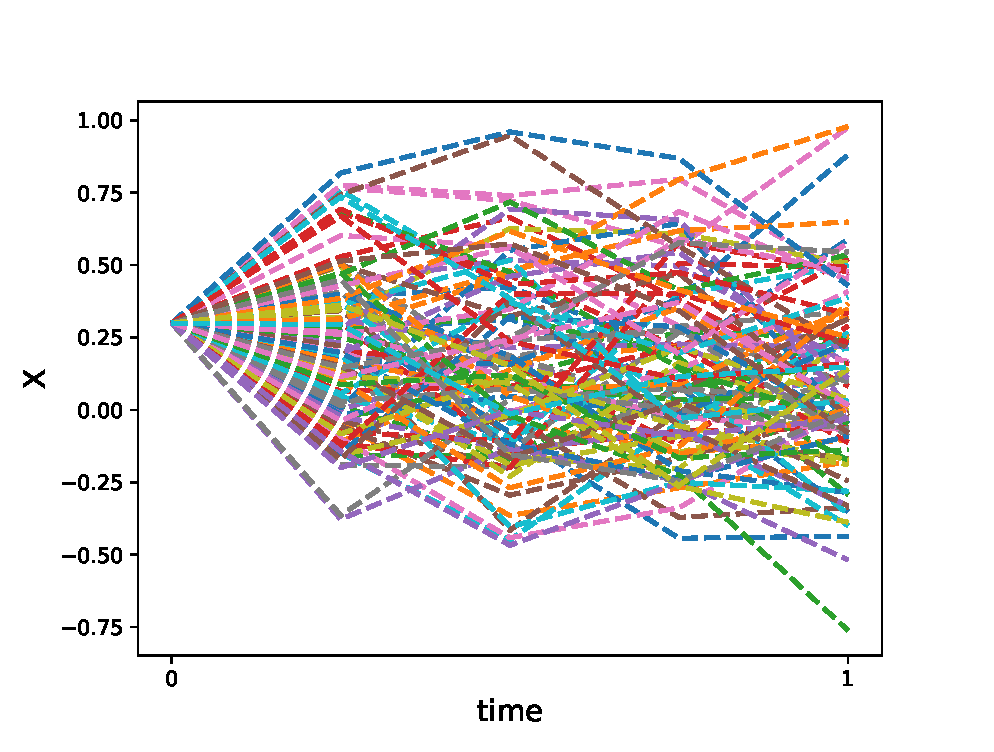
\includegraphics[width=\linewidth]{./figures/Heston_single_call_smooth_vol/paths_trajectory/paths_smooth_vol_scheme_set3_N4_X}
		\caption{}
		\label{fig:2}
	\end{subfigure}\hfil %% <-- added
	\caption{$100$ paths of process $X$ given by \eqref{equivalent OU process} simulated using forward Euler. (a) Case of set $1$ parameters in Table \ref{table:Reference solution, for different parameter constellations.}, (b) Case of set $3$ parameters in Table \ref{table:Reference solution, for different parameter constellations.}.}
	\label{fig:paths of process $X$ simulated using forward Euler}	
\end{figure}
\FloatBarrier

\item  Both schemes based on moment matching (ABR and QE schemes) have the best performance in terms of mixed rates convergence and also they show robust behavior with respect to all examples with almost similar performance
\end{enumerate}
 
 \subsubsection*{Mixed differences for the case of Set 1 parameters}
\FloatBarrier
\begin{figure}[htb]
	\centering % <-- added
	\begin{subfigure}{0.4\textwidth}
		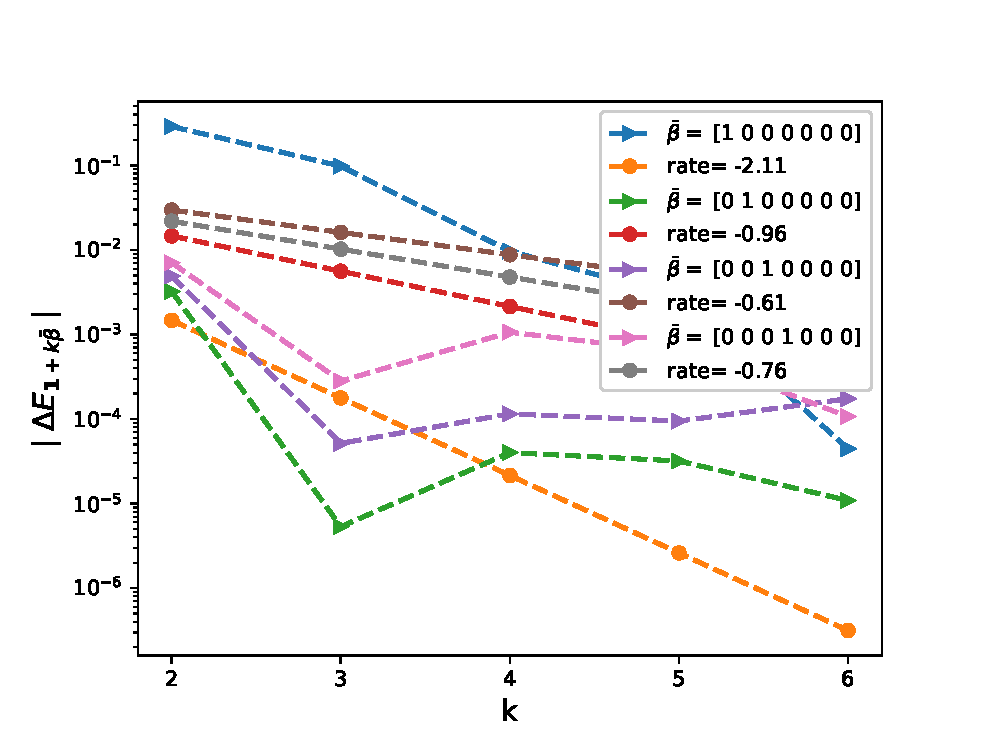
\includegraphics[width=\linewidth]{./figures/Heston_single_call_full_truncation_vol/mixed_rates/set2/N_4/first_difference_heston_4steps_hierarchical_2}
		\caption{}
		\label{fig:1}
	\end{subfigure}\hfil %% <-- added
	\begin{subfigure}{0.4\textwidth}
		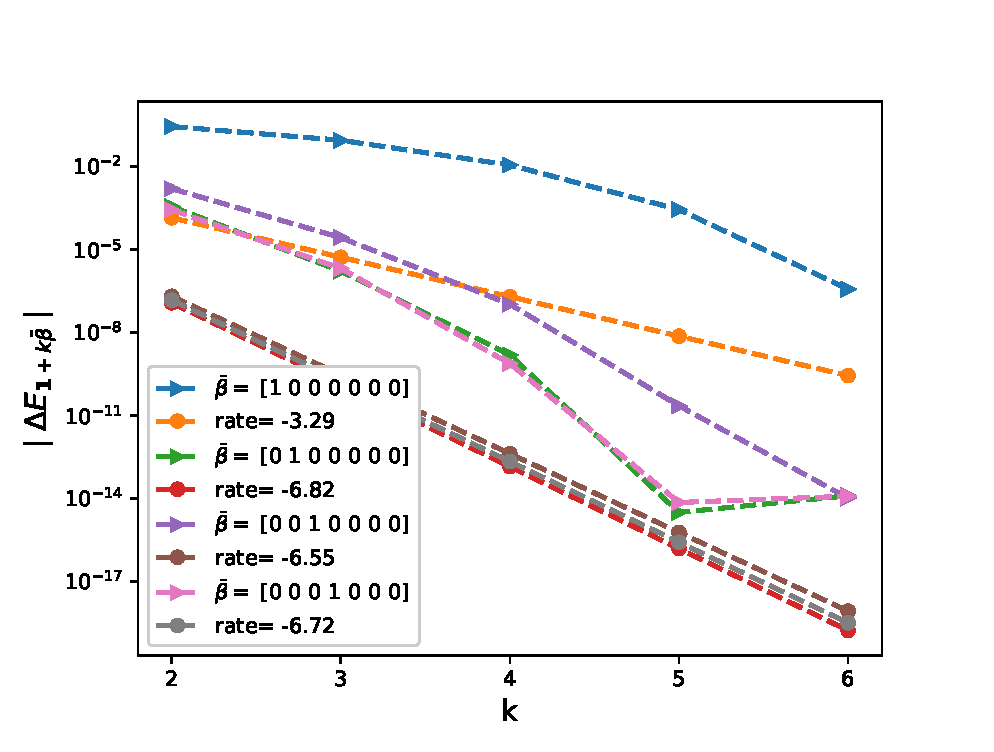
\includegraphics[width=\linewidth]{./figures/Heston_single_call_ABR_moment_matching/mixed_rates/set2/N_4/first_difference_heston_4steps_hierarchical}
		\caption{}
		\label{fig:2}
	\end{subfigure}\hfil %% <-- added
	\begin{subfigure}{0.4\textwidth}
		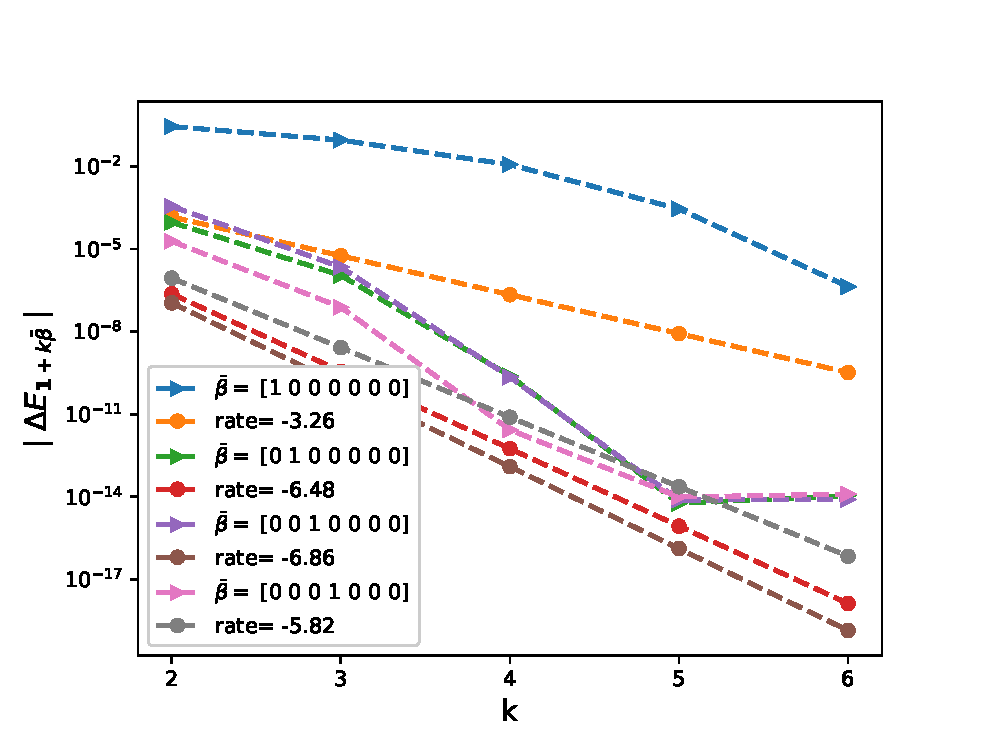
\includegraphics[width=\linewidth]{./figures/Heston_single_call_QE_moment_matching/mixed_rates/set2/N_4/first_difference_heston_4steps_hierarchical}
		\caption{}
		\label{fig:3}
	\end{subfigure}
		\begin{subfigure}{0.4\textwidth}
		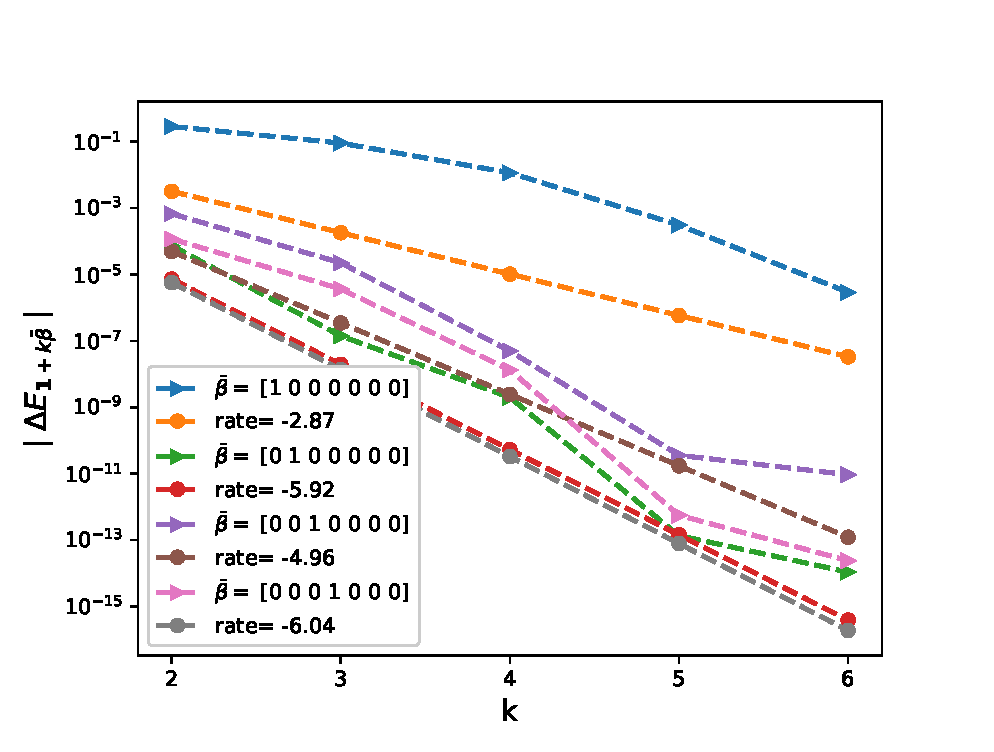
\includegraphics[width=\linewidth]{./figures/Heston_single_call_smooth_vol/mixed_rates/set2/N_4/first_difference_heston_4steps_spot_hierarchical_2}
		\caption{}
		\label{fig:4}
	\end{subfigure}
	\caption{The rate of error convergence of first order differences $\abs{\Delta \text{E}_{\boldsymbol{\beta}}}$, defined by \eqref{eq:Work_error_contributions}, ($\boldsymbol{\beta}=\mathbf{1}+k \bar{\boldsymbol{\beta}}$) for the example of single call option under Heston model, with parameters given by Set $1$ in Table \ref{table:Reference solution, for different parameter constellations.},  using $N=4$ time steps. In this case, we just show  the first  $4$ dimensions which are used for the volatility noise (mainly $dW_v$ in \eqref{eq:dynamics Heston}). (a) using full truncation as in Section \ref{sec:Discretization of Heston model with a non smooth transformations for the volatility process}, (b) using the ABR scheme as in Section \ref{sec:The ABR method}, (c) using the QE scheme as in Section \ref{sec:The QE method}, (d) using the smooth transformation as in Section \ref{sec:Discretization of Heston model with the volatility process Simulated using the sum of  Ornstein-Uhlenbeck (Bessel) processes}.}
	\label{fig:first_diff_Heston_call_N_4_set2}	
\end{figure}
\FloatBarrier


\subsubsection*{Mixed differences for the case of Set 2 parameters}

\FloatBarrier
\begin{figure}[htb]
	\centering % <-- added
	\begin{subfigure}{0.4\textwidth}
		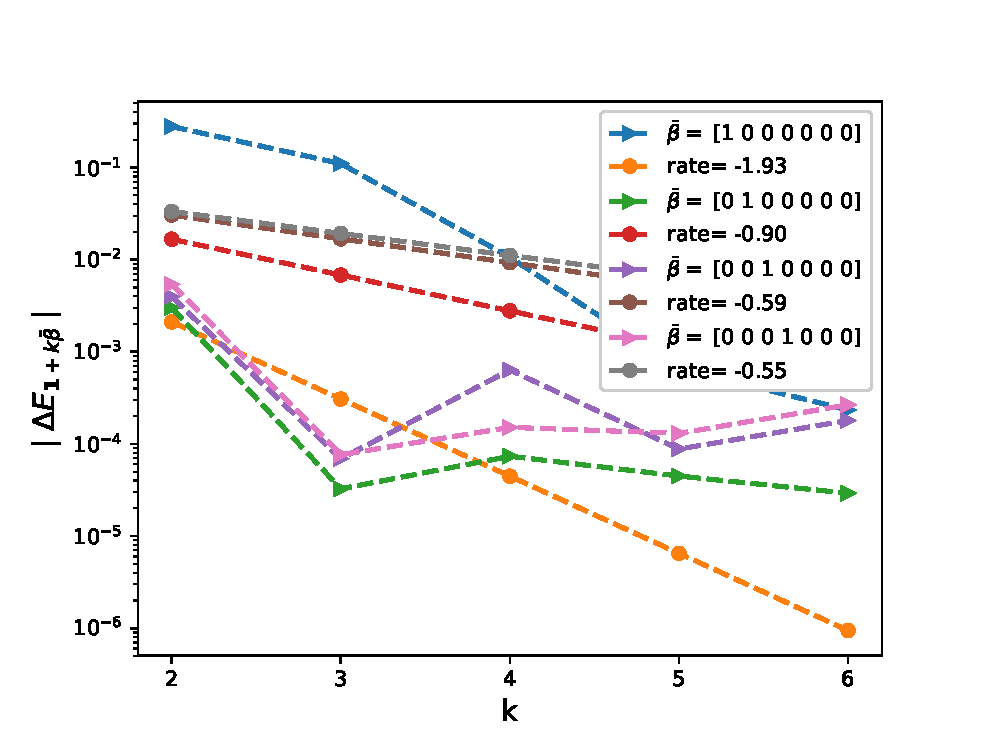
\includegraphics[width=\linewidth]{./figures/Heston_single_call_full_truncation_vol/mixed_rates/set3/N_4/first_difference_heston_4steps_hierarchical}
		\caption{}
		\label{fig:1}
	\end{subfigure}\hfil % <-- added
	\begin{subfigure}{0.4\textwidth}
		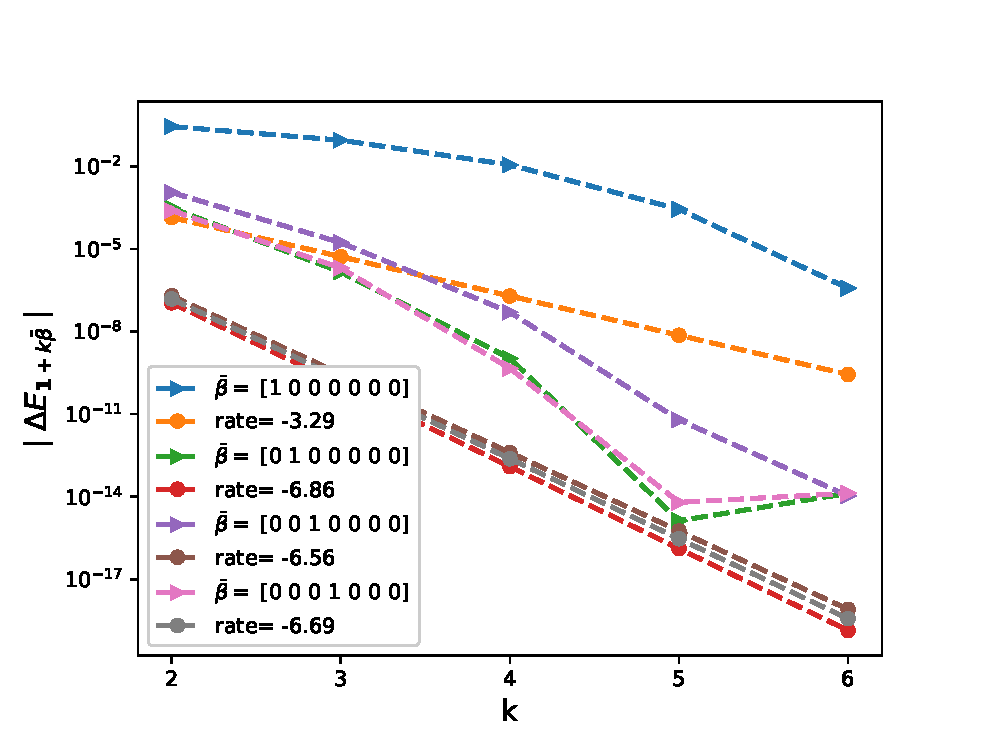
\includegraphics[width=\linewidth]{./figures/Heston_single_call_ABR_moment_matching/mixed_rates/set3/N_4/first_difference_heston_4steps_hierarchical}
		\caption{}
		\label{fig:2}
	\end{subfigure}\hfil % <-- added
	\begin{subfigure}{0.4\textwidth}
		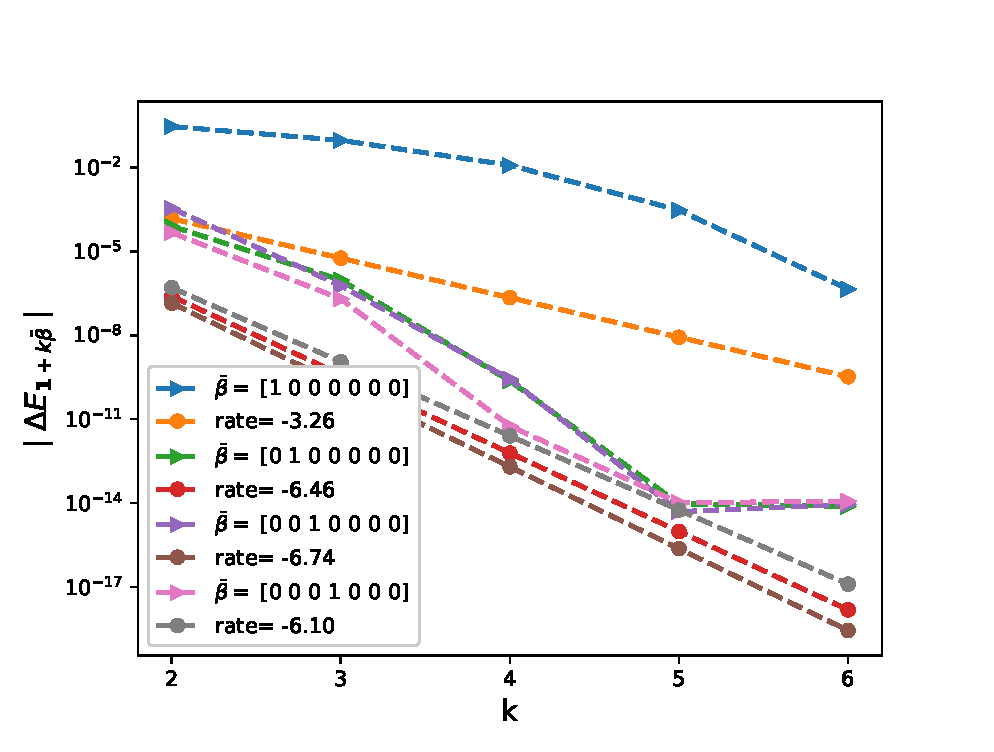
\includegraphics[width=\linewidth]{./figures/Heston_single_call_QE_moment_matching/mixed_rates/set3/N_4/first_difference_heston_4steps_hierarchical}
		\caption{}
		\label{fig:3}
	\end{subfigure}
		\begin{subfigure}{0.4\textwidth}
		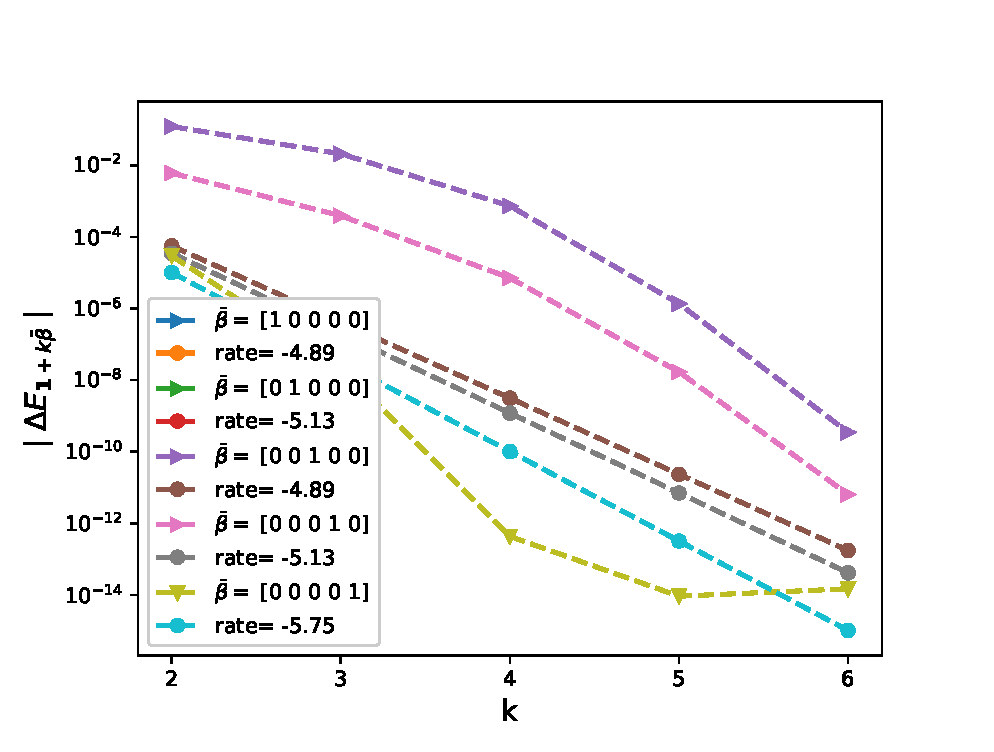
\includegraphics[width=\linewidth]{./figures/Heston_single_call_smooth_vol/mixed_rates/set3/N_2/first_difference_heston_2steps_spot_hierarchical}
		\caption{}
		\label{fig:4}
	\end{subfigure}
	\caption{The rate of error convergence of first order differences $\abs{\Delta \text{E}_{\boldsymbol{\beta}}}$, defined by \eqref{eq:Work_error_contributions}, ($\boldsymbol{\beta}=\mathbf{1}+k \bar{\boldsymbol{\beta}}$) for the example of single call option under Heston model, with parameters given by Set $2$ in Table \ref{table:Reference solution, for different parameter constellations.}, using $N=4$ time steps. In this case, we just show  the first  $4$ dimensions which are used for the volatility noise (mainly $dW_v$ in \eqref{eq:dynamics Heston}). (a) using full truncation as in Section \ref{sec:Discretization of Heston model with a non smooth transformations for the volatility process}, (b) using the ABR scheme as in Section \ref{sec:The ABR method}, (c) using the QE scheme as in Section \ref{sec:The QE method}, (d) using the smooth transformation as in Section \ref{sec:Discretization of Heston model with the volatility process Simulated using the sum of  Ornstein-Uhlenbeck (Bessel) processes}, here $N=2$.}
	\label{fig:first_diff_Heston_call_N_4_set3}	
\end{figure}
\FloatBarrier
\subsubsection*{Mixed differences for the case of Set 3 parameters}

\FloatBarrier
\begin{figure}[htb]
	\centering % <-- added
	\begin{subfigure}{0.4\textwidth}
		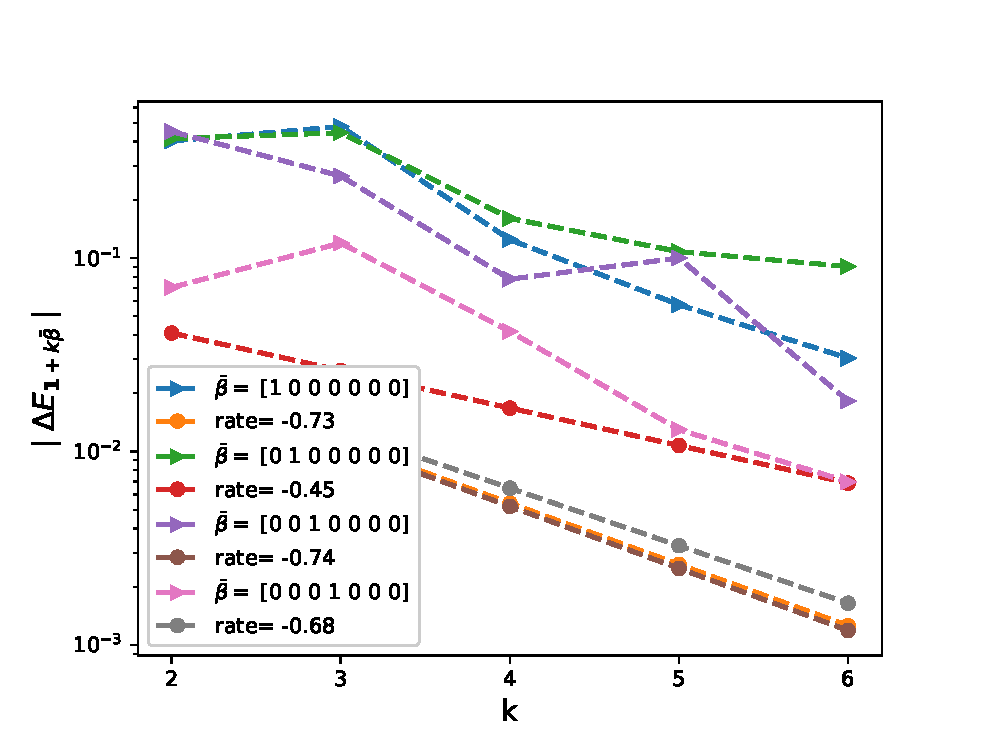
\includegraphics[width=\linewidth]{./figures/Heston_single_call_full_truncation_vol/mixed_rates/set4/N_4/first_difference_heston_4steps_hierarchical}
		\caption{}
		\label{fig:1}
	\end{subfigure}\hfil % <-- added
	\begin{subfigure}{0.4\textwidth}
		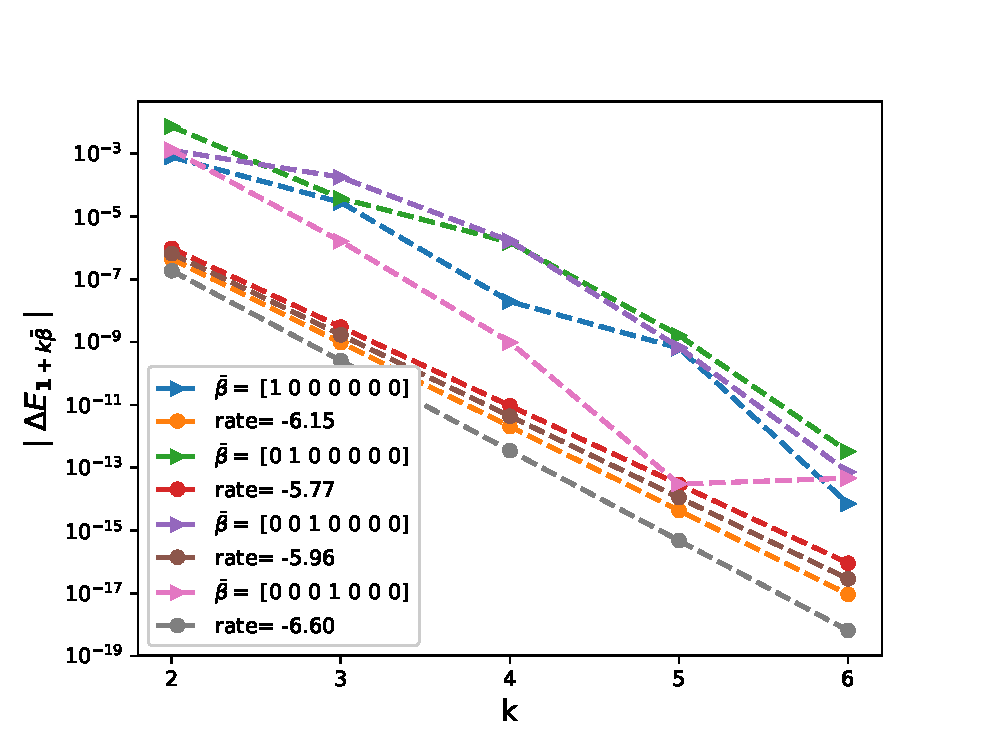
\includegraphics[width=\linewidth]{./figures/Heston_single_call_ABR_moment_matching/mixed_rates/set4/N_4/first_difference_heston_4steps_hierarchical}
		\caption{}
		\label{fig:2}
	\end{subfigure}\hfil % <-- added
	\begin{subfigure}{0.4\textwidth}
		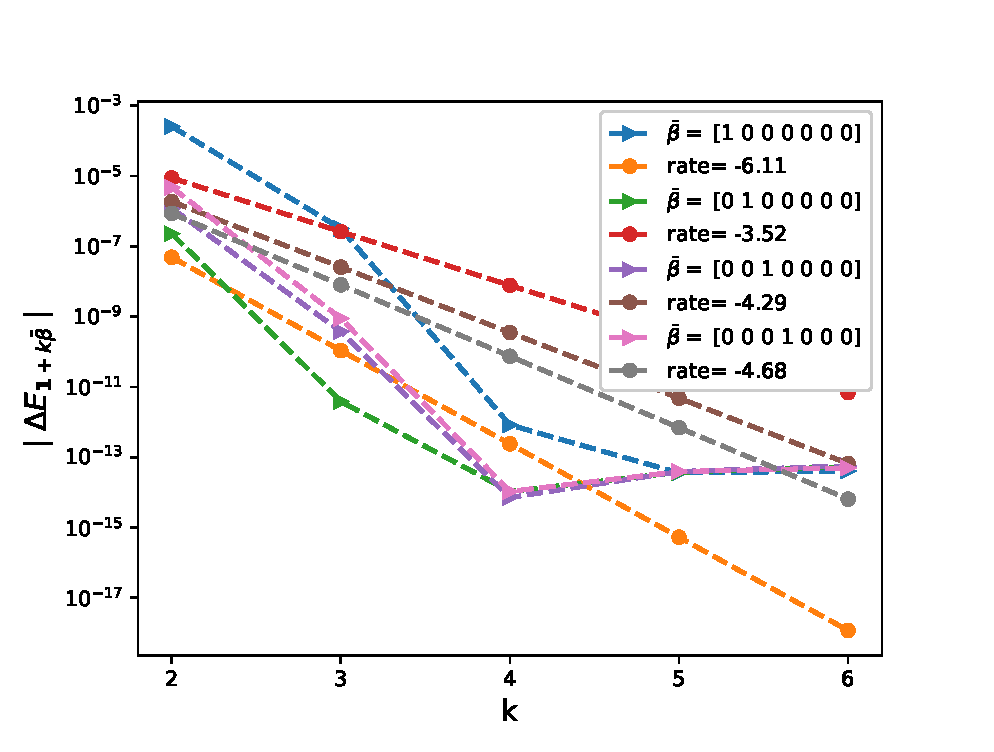
\includegraphics[width=\linewidth]{./figures/Heston_single_call_QE_moment_matching/mixed_rates/set4/N_4/first_difference_heston_4steps_hierarchical}
		\caption{}
		\label{fig:3}
	\end{subfigure}
		\begin{subfigure}{0.4\textwidth}
		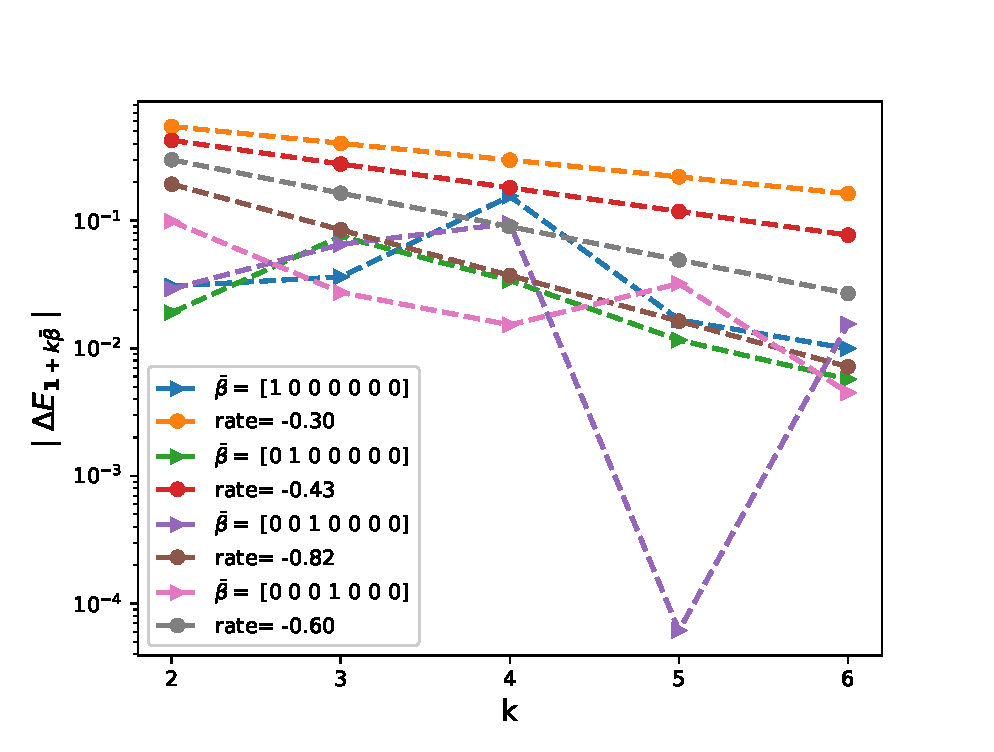
\includegraphics[width=\linewidth]{./figures/Heston_single_call_smooth_vol/mixed_rates/set4/N_4/first_difference_heston_4steps_spot_hierarchical}
		\caption{}
		\label{fig:4}
	\end{subfigure}
	\caption{The rate of error convergence of first order differences $\abs{\Delta \text{E}_{\boldsymbol{\beta}}}$, defined by \eqref{eq:Work_error_contributions}, ($\boldsymbol{\beta}=\mathbf{1}+k \bar{\boldsymbol{\beta}}$) for the example of single call option under Heston model, with parameters given by Set $3$ in Table \ref{table:Reference solution, for different parameter constellations.}, using $N=4$ time steps. In this case, we just show  the first  $4$ dimensions which are used for the volatility noise (mainly $dW_v$ in \eqref{eq:dynamics Heston}). (a) using full truncation as in Section \ref{sec:Discretization of Heston model with a non smooth transformations for the volatility process}, (b) using the ABR scheme as in Section \ref{sec:The ABR method}, (c) using the QE scheme as in Section \ref{sec:The QE method}, (d) using the smooth transformation as in Section \ref{sec:Discretization of Heston model with the volatility process Simulated using the sum of  Ornstein-Uhlenbeck (Bessel) processes}.}
	\label{fig:first_diff_Heston_call_N_4_set4}	
\end{figure}
\FloatBarrier
  
\subsubsection*{Mixed differences for the case of Set 4 parameters}

\FloatBarrier
\begin{figure}[htb]
	\centering % <-- added
	\begin{subfigure}{0.4\textwidth}
		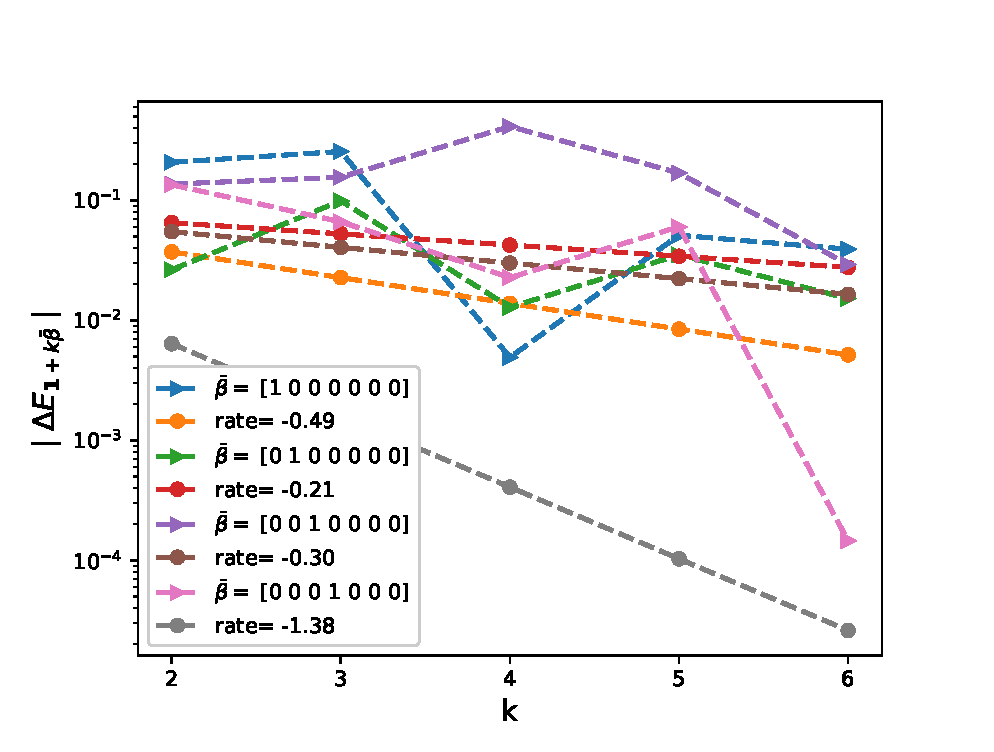
\includegraphics[width=\linewidth]{./figures/Heston_single_call_full_truncation_vol/mixed_rates/set5/N_4/first_difference_heston_4steps_hierarchical}
		\caption{}
		\label{fig:1}
	\end{subfigure}\hfil % <-- added
	\begin{subfigure}{0.4\textwidth}
		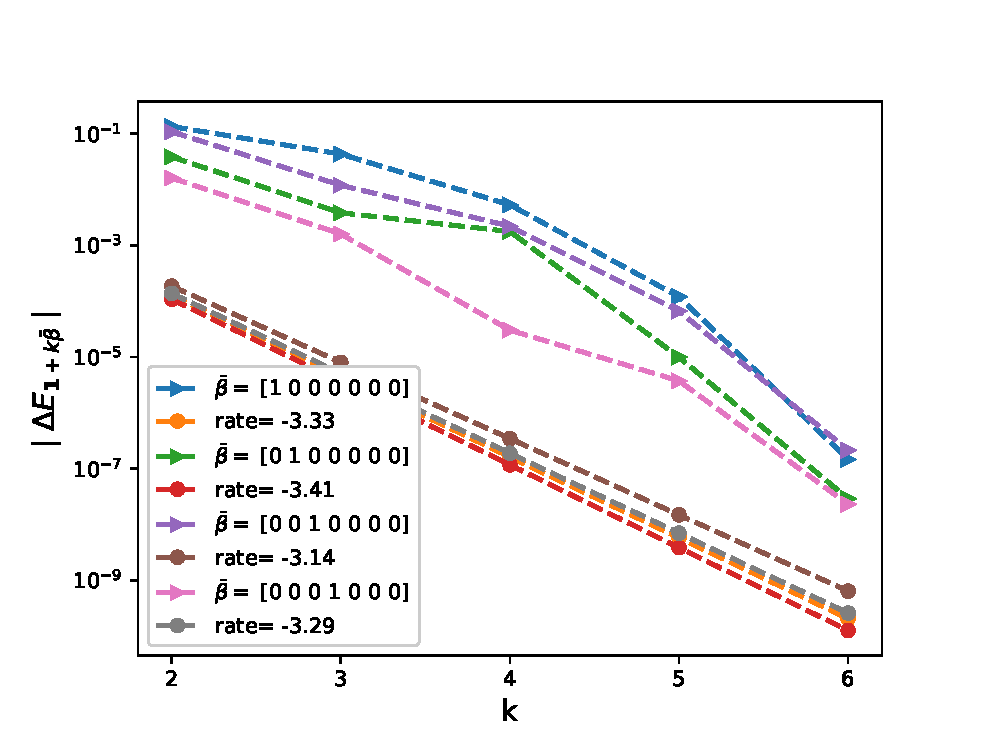
\includegraphics[width=\linewidth]{./figures/Heston_single_call_ABR_moment_matching/mixed_rates/set5/N_4/first_difference_heston_4steps_hierarchical}
		\caption{}
		\label{fig:2}
	\end{subfigure}\hfil % <-- added
		\begin{subfigure}{0.4\textwidth}
		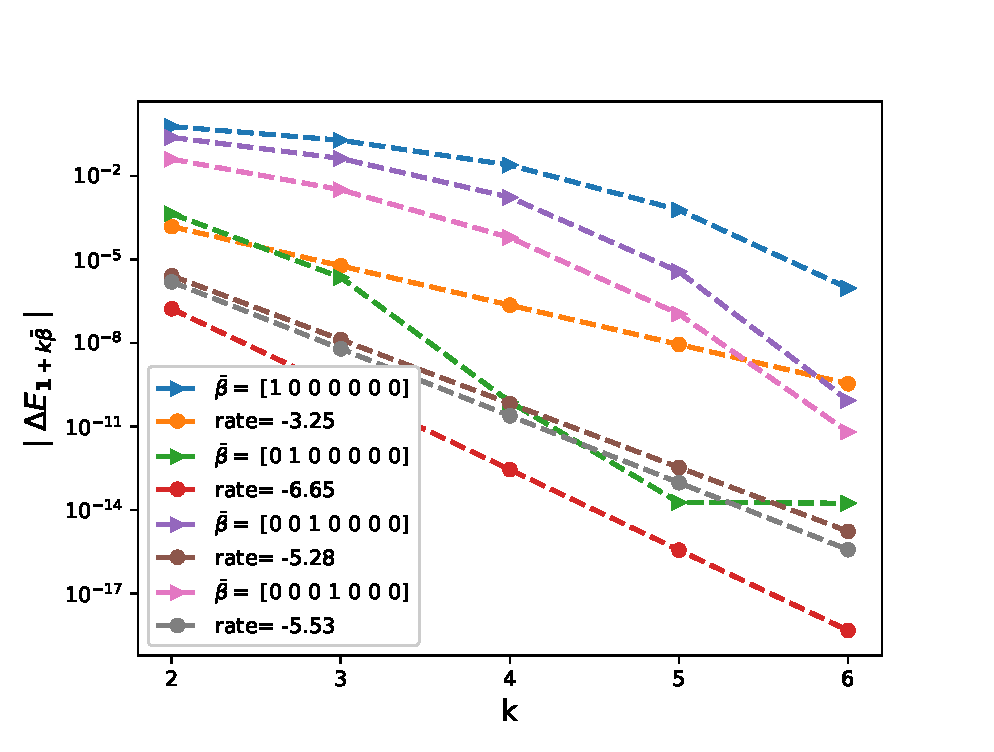
\includegraphics[width=\linewidth]{./figures/Heston_single_call_QE_moment_matching/mixed_rates/set5/N_4/first_difference_heston_4steps_hierarchical}
		\caption{}
		\label{fig:3}
	\end{subfigure}
	\caption{The rate of error convergence of first order differences $\abs{\Delta \text{E}_{\boldsymbol{\beta}}}$, defined by \eqref{eq:Work_error_contributions}, ($\boldsymbol{\beta}=\mathbf{1}+k \bar{\boldsymbol{\beta}}$) for the example of single call option under Heston model, with parameters given by Set $4$ in Table \ref{table:Reference solution, for different parameter constellations.}, using $N=4$ time steps. In this case, we just show  the first  $4$ dimensions which are used for the volatility noise (mainly $dW_v$ in \eqref{eq:dynamics Heston}).(a) using full truncation as in Section \ref{sec:Discretization of Heston model with a non smooth transformations for the volatility process}, (b) using the ABR scheme as in Section \ref{sec:The ABR method}, (c) using the QE scheme as in Section \ref{sec:The QE method}.}
	\label{fig:first_diff_Heston_call_N_4_set5}	
\end{figure}
\FloatBarrier

\subsubsection{Comparison in terms of  the weak error behavior}
\subsubsection*{Weak error behavior for the case of Set 1 parameters}


\FloatBarrier
\begin{figure}[htb]
	\centering % <-- added
	\begin{subfigure}{0.4\textwidth}
		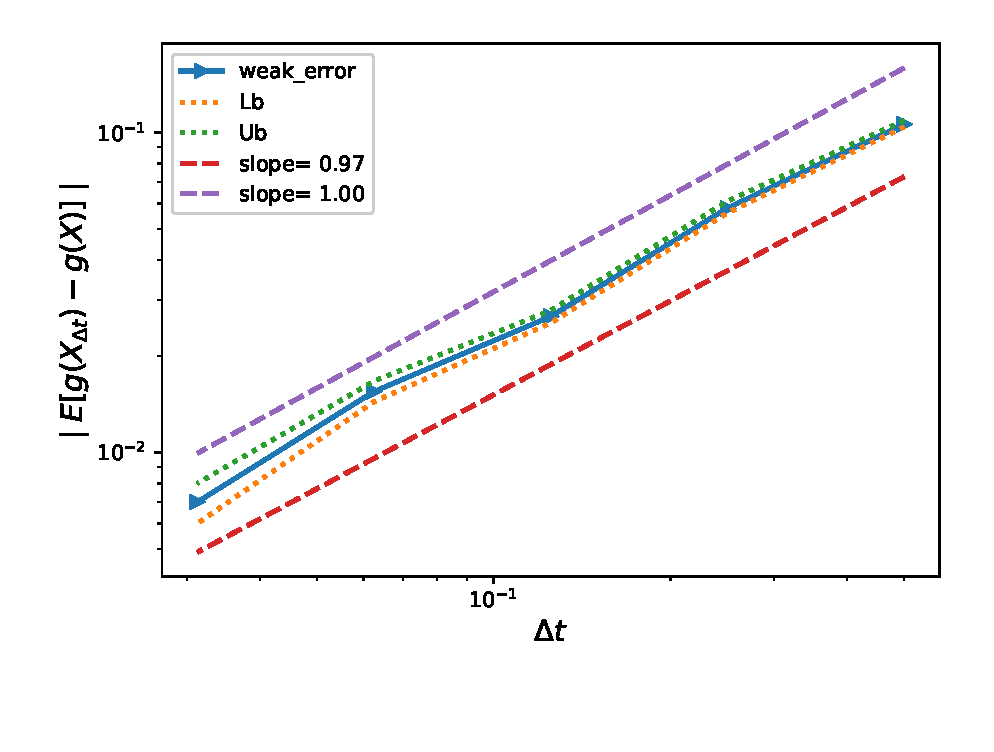
\includegraphics[width=\linewidth]{./figures/Heston_single_call_smooth_vol/weak_convergence/weak_convergence_order_single_call_option_heston_relative_M_4_10_6_beta_512_smooth_scheme_set1}
		\caption{}
		\label{fig:1}
	\end{subfigure}\hfil %% <-- added
	\begin{subfigure}{0.4\textwidth}
		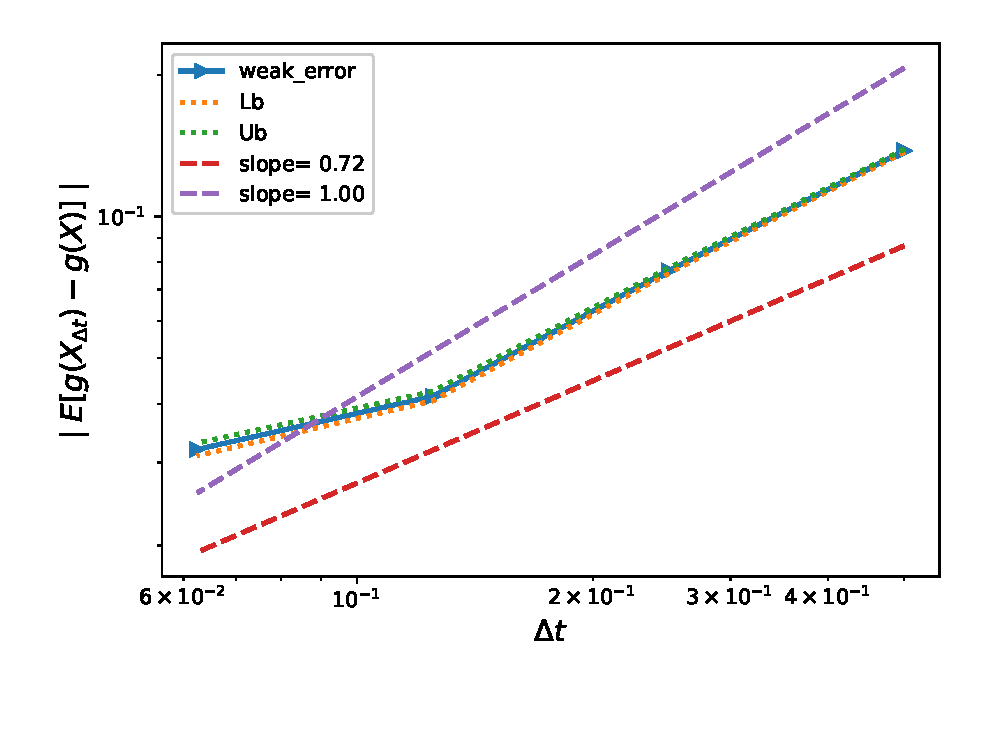
\includegraphics[width=\linewidth]{./figures/Heston_single_call_ABR_moment_matching/weak_convergence/weak_convergence_order_single_call_option_heston_relative_M_1_10_7_beta_128_ABR_set1}
		\caption{}
		\label{fig:2}
	\end{subfigure}\hfil %% <-- added
	\caption{The convergence of the relative weak error  $\mathcal{E}_B(N)$ defined in \ref{eq:total_error}, for the European call option  under the discretized  Heston model, for Set $1$ parameters in Table \ref{table:Reference solution, for different parameter constellations.}. The upper and lower bounds are $95\%$ confidence intervals. (a) using the smooth transformation as in Section \ref{sec:Discretization of Heston model with the volatility process Simulated using the sum of  Ornstein-Uhlenbeck (Bessel) processes}, (b) using the ABR scheme as in Section \ref{sec:The ABR method}.}
	\label{fig:weak convergence comparison set 1}	
\end{figure}
\FloatBarrier
\subsubsection*{Weak error behavior for the case of Set 2 parameters}


\FloatBarrier
\begin{figure}[htb]
	\centering % <-- added
	\begin{subfigure}{0.4\textwidth}
		\includegraphics[width=\linewidth]{./figures/Heston_single_call_smooth_vol/weak_convergence/paths_smooth_vol_scheme_set1_N4_X}
		\caption{}
		\label{fig:1}
	\end{subfigure}\hfil %% <-- added
	\begin{subfigure}{0.4\textwidth}
		\includegraphics[width=\linewidth]{./figures/Heston_single_call_ABR_moment_matching/weak_convergence/weak_convergence_order_single_call_option_heston_relative_M_1_10_7_beta_128_ABR_set2}
		\caption{}
		\label{fig:2}
	\end{subfigure}\hfil %% <-- added
	\caption{The convergence of the relative weak error  $\mathcal{E}_B(N)$ defined in \ref{eq:total_error}, for the European call option  under the discretized  Heston model, for Set $2$ parameters in Table \ref{table:Reference solution, for different parameter constellations.}. The upper and lower bounds are $95\%$ confidence intervals. (a) using the smooth transformation as in Section \ref{sec:Discretization of Heston model with the volatility process Simulated using the sum of  Ornstein-Uhlenbeck (Bessel) processes}, (b) using the ABR scheme as in Section \ref{sec:The ABR method}.}
	\label{fig:weak convergence comparison set 2}	
\end{figure}
\FloatBarrier

\subsubsection*{Weak error behavior for the case of Set 3 parameters}


\FloatBarrier
\begin{figure}[htb]
	\centering % <-- added
		\includegraphics[width=0.5\linewidth]{./figures/Heston_single_call_ABR_moment_matching/weak_convergence/weak_convergence_order_single_call_option_heston_relative_M_1_10_7_beta_128_ABR_set3}
	\caption{The convergence of the relative weak error  $\mathcal{E}_B(N)$ defined in \ref{eq:total_error},using the ABR scheme as in Section \ref{sec:The ABR method}, for the European call option  under the discretized  Heston model, for Set $3$ parameters in Table \ref{table:Reference solution, for different parameter constellations.}. The upper and lower bounds are $95\%$ confidence intervals.}
	\label{fig:weak convergence comparison set 3}	
\end{figure}
\FloatBarrier
\subsubsection{European call option  under the discretized  Heston model with parameters of Set $1$ in Table \ref{table:Reference solution, for different parameter constellations.}}\label{sec:European call option  under the discretized  Heston model with parameters of Set 1}
We consider now  the European call option  under the discretized  Heston model  with parameters given by Set $1$ in Table \ref{table:Reference solution, for different parameter constellations.}. In this case, we use the smooth scheme described  in  Section \ref{sec:Discretization of Heston model with the volatility process Simulated using the sum of  Ornstein-Uhlenbeck (Bessel) processes} and with  $n=1$ (that is we just use one OU process to simulate the volatility). Figure \ref{fig:Weak_rate_call_heston_smooth_vol} shows the estimated weak error  for the case without Richardson extrapolation, and we report the results for comparing MC (we used the Full truncation scheme to simulate the volatility) and ASGQ (we used the smooth approach in Section \ref{sec:Discretization of Heston model with the volatility process Simulated using the sum of  Ornstein-Uhlenbeck (Bessel) processes} to simulate the volatility) in Tables \ref{Total error of MISC and MC to compute European call option price under discretized Heston model of the different tolerances for different number of time steps, without Richardson extrapolation. The numbers between parentheses are the corresponding absolute errors.} and \ref{Comparsion of the computational time of  MC and MISC, used to compute European call option price under discretized Heston model for different number of time steps, without Richardson extrapolation} for the case without Richardson extrapolation, and  Tables \ref{Total relative  error of ASGQ  to compute European call option price under discretized Heston model for different number of time steps, with level $1$ of Richardson extrapolation. The values between parentheses correspond to the different errors contributing to the total relative error: for ASGQ we report the bias and quadrature errors.} and \ref{table:The computational time of  ASGQ, used to compute European call option price under discretized Heston model for different number of time steps, with level $1$ Richardson extrapolation.} for the case of level $1$ Richardson extrapolation. We also compare the performance of the two methods for different configurations in  Figure \ref{fig:Complexity plot for MC and MISC , European call option price under discretized Heston model}.  Our numerical experiments show that Richardson extrapolation improved the performance of both ASGQ and MC, and that for achieving a relative error around $1.4\%$, ASGQ  coupled with level $1$ of Richardson extrapolation is the optimal method, and  requires approximately $33\%$ of the work of MC  coupled with level $1$ of Richardson extrapolation. 
 

\FloatBarrier
\begin{table}[h!]
	\centering
	\begin{tabular}{l*{6}{c}r}
		\toprule[1.5pt]
	Method & & Steps  & &  &    \\
	\hline
           & $2$ & $4$ & $8$   & $16$ & $32$ \\
		\hline
		ASGQ   &  $\underset{(0.106,0.009)}{\mathbf{0.115}}$ & $\underset{(0.058,0.016)}{\mathbf{0.0740}}$ & $\underset{(0.0266,0.0213)}{\mathbf{0.0479}}$ & $\underset{(0.0155,0.0127)}{\mathbf{0.0282}}$ & $\underset{(0.007,0.008)}{\mathbf{0.015}}$   \\
		\hline		
%			MC +root finding   &  $\underset{(0.106,.)}{\mathbf{}}$ & $\underset{(0.058,)}{\mathbf{}}$ & $\underset{(0.0266,)}{\mathbf{.}}$ & $\underset{(0.0155,)}{\mathbf{.}}$ & $\underset{(0.007,)}{\mathbf{}}$   \\
%			M(\# MC samples)   & $.$   &  $.$ &  $.$ &  $.$  \\	
%		\hline	
				MC   &  $\underset{(0.106,0.106)}{\mathbf{0.212}}$ & $\underset{(0.058,0.057)}{\mathbf{ 0.115}}$ & $\underset{(0.0266,0.0262)}{\mathbf{
    0.0528}}$ & $\underset{(0.0155,0.013)}{\mathbf{0.0285}}$  & $\underset{(0.007,0.0072)}{\mathbf{0.0142}}$   \\ 
				M(\# MC samples)   &$10^3$  & $3 \times 10^3$  &  $2 \times 10^4$ &  $6 \times 10^4 $ &  $2 \times 10^5$\\	
			\bottomrule[1.25pt]
	\end{tabular}
	\caption{Total relative  error of ASGQ, with different tolerances, and MC to compute European call option price under discretized Heston model for different number of time steps, without Richardson extrapolation. The values between parentheses correspond to the different errors contributing to the total relative error: for ASGQ we report the bias and quadrature errors and for MC we report the bias and the statistical errors. The number of MC samples,$ M$, is chosen to satisfy \eqref{optimal_number_samples}.}
	\label{Total error of MISC and MC to compute European call option price under discretized Heston model of the different tolerances for different number of time steps, without Richardson extrapolation. The numbers between parentheses are the corresponding absolute errors.}
\end{table}
\FloatBarrier


\begin{table}[h!]
	\centering
	\begin{tabular}{l*{6}{c}r}
		\toprule[1.5pt]
	Method & & Steps  & &      &\\
	\hline
	         & $2$ & $4$ & $8$  & $16$  & $32$   \\
		\hline
		ASGQ & $14$  & $18$ & $24.5$ & $76.5$     & $351$    \\
%			MC  +root finding  & $.$&  $.$&  $.$ &  $.$ &  $.$    \\
				MC  &   $0.5$& $1.5$ &   $10$&   $50$&   $730$  \\
		\bottomrule[1.25pt]
	\end{tabular}
	\caption{Comparison of the computational time of  MC and ASGQ, used to compute European call option price under discretized Heston model for different number of time steps, without Richardson extrapolation. The average computational time of MC is computed over $10$ runs.}
	\label{Comparsion of the computational time of  MC and MISC, used to compute European call option price under discretized Heston model for different number of time steps, without Richardson extrapolation}
\end{table}
\FloatBarrier



\begin{table}[h!]
	\centering
	\begin{tabular}{l*{6}{c}r}
		\toprule[1.5pt]
	Method & &   &Steps &  &   &    \\
	\hline
           & $1-2$ & $2-4$  & $4-8$   \\
		\hline
		ASGQ   &  $\underset{(0.037,0.01)}{\mathbf{0.038}}$ & $\underset{(0.0077,0.0065)}{\mathbf{0.0142}}$  & $\underset{(0.0015,0.0017)}{\mathbf{0.0032}}$ \\
		\hline
						MC   &  $\underset{(0.067,0.064)}{\mathbf{0.131}}$ & $\underset{(0.0061,0.0062)}{\mathbf{0.0123}}$ & $\underset{(0.0016,0.0015)}{\mathbf{0.0031}}$  \\ 
				M(\# MC samples)   &$2 \times 10^3$  &$3 \times 10^5$  &$4 \times 10^6$   \\	
			\bottomrule[1.25pt]
	\end{tabular}
	\caption{Total relative  error of ASGQ and MC to compute European call option price under discretized Heston model for different number of time steps, with level $1$ of Richardson extrapolation. The values between parentheses correspond to the different errors contributing to the total relative error: for ASGQ we report the bias and quadrature errors and for MC we report the bias and the statistical errors. The number of MC samples,$ M$, is chosen to satisfy \eqref{optimal_number_samples}.}
	\label{Total relative  error of ASGQ  to compute European call option price under discretized Heston model for different number of time steps, with level $1$ of Richardson extrapolation. The values between parentheses correspond to the different errors contributing to the total relative error: for ASGQ we report the bias and quadrature errors.}
\end{table}
\FloatBarrier


\begin{table}[h!]
	\centering
	\begin{tabular}{l*{6}{c}r}
		\toprule[1.5pt]
	Method & & Steps  & &      &\\
	\hline
	         & $1-2$ & $2-4$  & $4-8$ \\
	         	\hline
		ASGQ & $4.5$  & $48.5$ & $864$  \\
				MC  &   $1$& $145$& $2764$   \\
		\bottomrule[1.25pt]
	\end{tabular}
	\caption{Comparison of the computational time of  MC and ASGQ, used to compute European call option price under discretized Heston model for different number of time steps, with level $1$ of Richardson extrapolation. The average computational time of MC is computed over $10$ runs.}
	\label{table:The computational time of  ASGQ, used to compute European call option price under discretized Heston model for different number of time steps, with level $1$ Richardson extrapolation.}
\end{table}


\FloatBarrier
	\begin{figure}[h!]
\centering
\includegraphics[width=0.5\linewidth]{./figures/Heston_single_call_smooth_vol/complexity_rates/set1/error_vs_time}

\caption{Computational work comparison for ASGQ and MC methods, for the case of European call option price under discretized Heston model. This plot shows that to achieve a relative error around $1.4\%$, using level $1$ of Richardson extrapolation is the optimal configuration for both methods, and that ASGQ coupled with level $1$ of Richardson extrapolation  outperforms  MC coupled with level $1$ of Richardson extrapolation  method in terms of computational time.}
\label{fig:Complexity plot for MC and MISC , European call option price under discretized Heston model}
\end{figure}
\FloatBarrier



\section{Numerical smoothing with MLMC}
In this section, we want to motivate the advantage of the numerical smoothing idea in the context of MLMC method. For this aim we consider two examples: i) the first one is for computing the price of a digital option (see Section \ref{sec: MLMC for digital options}) , and ii) the second example is for approximating a density function with application to computing Greeks of options having non smooth payoff (see Section \ref{sec: MLMC for approximating densities and greeks}). The results  of the first example can be generalized for any kind of option having low regularity in the payoff function. On the other hand, the second example have two important applications: i) computing density functions which involves the use of Dirac functions and which is hard to approximate its expectation using MLMC due to the infinite variance, and ii) computing Greeks for an option with a non smooth payoff function.


\subsection{MLMC for digital options}\label{sec: MLMC for digital options}
In this section, we motivate the idea of using the numerical smoothing idea to compute option prices for non smooth payoff function. As an illustration, we choose the digital option as an example with parameters: $S_0=K=100$, $T=1$, $r= 0$, and   $\sigma=0.2$, and we compare MLMC results with the original payoff function (without numerical smoothing), given by Figure \ref{fig:euler_digital_without_smoothing},  and MLMC results after applying our numerical smoothing idea, given by Figure \ref{fig:euler_digital_with_smoothing}. From these two Figures we have the following conclusions:
\begin{enumerate}
\item The numerical smoothing has improved the rate of strong convergence from $1/2$ (without smoothing) to $1$ after doing the numerical smoothing (compare both top left plots in Figures \ref{fig:euler_digital_without_smoothing} and Figure \ref{fig:euler_digital_with_smoothing}.
\item The numerical smoothing has also dropped significantly the kurtosis by a factor $100$, this is can be seen clearly by comparing the middle right plots in both Figures \ref{fig:euler_digital_without_smoothing} and Figure \ref{fig:euler_digital_with_smoothing}.
\item Finally, improving the strong error rate after using the numerical smoothing, resulted in an improvement of the complexity rate going from $TOL^{-2.5}$ for the case without smoothing to  $TOL^{-2} \abs{\log TOL}^2$ for the case where MLMC is coupled with numerical smoothing (compare the bottom right plots in Figures \ref{fig:euler_digital_without_smoothing} and \ref{fig:euler_digital_with_smoothing}).
\end{enumerate}

\FloatBarrier
	\begin{figure}[h!]
\centering
\includegraphics[width=1\linewidth]{./figures/MLMC_binary_opt/euler_digital_without_smoothing}

\caption{Numerical results for a digital call option using the MLMC method coupled with Euler-Maruyama discretisation of the GBM SDE, and without smoothing of the payoff.}
\label{fig:euler_digital_without_smoothing}
\end{figure}

\FloatBarrier

\FloatBarrier
	\begin{figure}[h!]
\centering
\includegraphics[width=0.7\linewidth]{./figures/MLMC_binary_opt/digital_option_with_smoothing_L_0_2_steps}

\caption{Numerical results for a digital call option using the MLMC method coupled with Euler-Maruyama discretisation of the GBM SDE, after applying  the numerical smoothing to the payoff.}
\label{fig:euler_digital_with_smoothing}
\end{figure}

\FloatBarrier


\subsection{MLMC for approximating densities and Greeks}\label{sec: MLMC for approximating densities and greeks}


 %%%%%%%%%%%%%%%%%%%%%%%%%%%%%%%%%%%%%%%%%%
%References
%%%%%%%%%%%%%%%%%%%%%%%%%%%%%%%%%%%%%%%%%%

\bibliographystyle{plain}
\bibliography{smoothing} 


%\appendix
%\section{Numerical comparison between MISC and MC}
\subsection{Case of set $1$ parameters in table \ref{table:Reference solution, using MC with $500$ time steps, of Call option price under rBergomi model, for different parameter constellation.}}\label{appendix:Case of set 1 parameters}


\begin{table}[h!]
	\centering
	\begin{tabular}{l*{6}{c}r}
		Method \textbackslash  Steps            & $2$ & $4$ & $8$ & $16$  \\
		\hline
%		MISC ($TOL_{\text{MISC}}=5.10^{-1}$)  & $\underset{0.0062}{\mathbf{  0.0868}}$ & $\underset{ 0.0040}{\mathbf{0.0563}}$ & $\underset{ 0.0040}{\mathbf{0.0563}}$ & $\underset{0.0014}{\mathbf{0.0197}}$  \\
		MISC ($TOL_{\text{MISC}}=10^{-1}$)  & $\underset{0.0062}{\mathbf{  0.0868}}$ & $\underset{ 0.0040}{\mathbf{0.0563}}$& $\underset{0.0049}{\mathbf{0.0681}}$ & $\underset{0.0035
		}{\mathbf{0.0492}}$  \\
%		MISC ($TOL_{\text{MISC}}=5.10^{-2}$)  &$\underset{0.0062}{\mathbf{  0.0868}}$ & $\underset{0.0042}{\mathbf{0.0591}}$ & $\underset{0.0021}{\mathbf{0.0288
%		}}$ & $\underset{0.0057}{\mathbf{0.0800}}$  \\
		MISC ($TOL_{\text{MISC}}=10^{-2}$)  & $\underset{ 0.0001
		}{\mathbf{\red{  0.0017}}}$ & $\underset{ 0.0023}{\mathbf{ 0.0324}}$ & $\underset{0.0016
		}{\mathbf{0.0218
		}}$ & $\underset{0.0005}{\mathbf{\red{0.0070}}}$  \\
		MISC ($TOL_{\text{MISC}}=10^{-3}$)  & $\underset{ 0.0001
		}{\mathbf{  0.0017}}$ & $\underset{1.0e-05
		}{\mathbf{ \red{1.4e-04
		}}}$ & $\underset{3.5e-04
		}{\mathbf{  0.0049
		}}$ & $\underset{0.0005}{\mathbf{ 0.0070}}$  \\
%		MISC ($TOL_{\text{MISC}}=5.10^{-4}$)  & $\underset{ 0.0001
%		}{\mathbf{  0.0017}}$ & $\underset{1.0e-05
%		}{\mathbf{ 1.4e-04
%		}}$ & $\underset{1.5e-04
%		}{\mathbf{    0.0021
%		}}$ & $\underset{-}{\mathbf{-}}$  \\
		MISC ($TOL_{\text{MISC}}=10^{-4}$)  & $\underset{ 0.0001
		}{\mathbf{  0.0017}}$ & $\underset{1.0e-05
		}{\mathbf{ 1.4e-04
		}}$ & $\underset{(  4.9e-05)
		}{\mathbf{\red{6.9e-04}
		}}$ & $\underset{-}{\mathbf{-}}$  \\
		\hline
	\end{tabular}
	\caption{Quadrature error of MISC,  with different tolerances, to compute call option price for different number of time steps. Case  set $1$ parameters in table \ref{table:Reference solution, using MC with $500$ time steps, of Call option price under rBergomi model, for different parameter constellation.}, without Richardson extrapolation. The numbers between parentheses are the corresponding absolute errors. The values marked in red correspond to stable quadrature errors for MISC, and will be used for complexity comparison against MC.}
	\label{Quadrature error of MISC to compute Call option price of the different tolerances for different number of time steps. Case  set $1$ parameters, without Richardson extrapolation. The numbers between parentheses are the corresponding absolute errors.}
\end{table}



\begin{table}[!h]
	\centering
	\begin{tabular}{l*{6}{c}r}
		Method \textbackslash  Steps            & $1-2$ & $2-4$ & $4-8$  \\
		\hline
%		MISC ($TOL_{\text{MISC}}=5.10^{-1}$)  & $\underset{(  0.0120)}{\mathbf{   0.1685}}$ & $\underset{(0.0031)}{\mathbf{0.0435}}$ & $\underset{(0.0014
%			)}{\mathbf{ 0.0197}}$  \\
		MISC ($TOL_{\text{MISC}}=10^{-1}$)  & $\underset{(  0.0120)}{\mathbf{   0.1685}}$ & $\underset{(0.0031)}{\mathbf{0.0435}}$ & $\underset{(0.0064)}{\mathbf{0.0899}}$  \\
%		MISC ($TOL_{\text{MISC}}=5.10^{-2}$)  & $\underset{(  0.0120)}{\mathbf{   0.1685}}$ & $\underset{(0.0079)}{\mathbf{0.1109}}$ & $\underset{(0.0052)}{\mathbf{0.0730}}$   \\
		MISC ($TOL_{\text{MISC}}=10^{-2}$)  & $\underset{(7e-07)}{\mathbf{1e-05}}$ &    $\underset{(0.0029)}{\mathbf{0.0407}}$ & $\underset{(0.0024  )}{\mathbf{0.0337}}$  \\
		MISC ($TOL_{\text{MISC}}=10^{-3}$)  & $\underset{(0.0013)}{\mathbf{
				\red{0.0183}}}$ &    $\underset{(0.0014
			)}{\mathbf{\red{0.0197}}}$ & $\underset{(0.0001)}{\mathbf{ \red{0.0014}
		}}$   \\
		
%		MISC ($TOL_{\text{MISC}}=10^{-4}$)  & $\underset{(0.0013)}{\mathbf{
%				0.0183}}$ &    $\underset{(0.0011
%			
%			)}{\mathbf{0.0154}}$   \\
		\hline
	\end{tabular}
	\caption{Quadrature error of MISC, with different tolerances,  to compute call option price  for different number of time steps. Case set $1$ parameters in table \ref{table:Reference solution, using MC with $500$ time steps, of Call option price under rBergomi model, for different parameter constellation.}, with Richardson extrapolation(level $1$). The numbers between parentheses are the corresponding absolute errors. The values marked in red correspond to stable quadrature errors for MISC, and will be used for complexity comparison against MC.}
	\label{Quadrature error of MISC to compute Call option price of the different tolerances for different number of time steps. Case set $1$ parameters, with Richardson extrapolation(level $1$). The numbers between parentheses are the corresponding absolute errors.}
\end{table}





\begin{table}[!h]
	\centering
	\begin{tabular}{l*{6}{c}r}
		Method \textbackslash  Steps            & $1-2-4$ & $2-4-8$  \\
		\hline
%		MISC ($TOL_{\text{MISC}}=5.10^{-1}$)  & $\underset{(     0.0017)}{\mathbf{    0.0239}}$ & $\underset{(0.0009)}{\mathbf{0.0126}}$ \\
		MISC ($TOL_{\text{MISC}}=10^{-1}$)  & $\underset{(   0.0041)}{\mathbf{  0.0576}}$ & $\underset{(0.0037)}{\mathbf{0.0520}}$  \\
%		MISC ($TOl=5.10^{-2}$)  & $\underset{(  0.0125)}{\mathbf{   0.1755}}$ & $\underset{(0.0072)}{\mathbf{0.1011}}$   \\
		MISC ($TOL_{\text{MISC}}=10^{-2}$)  & $\underset{(0.0031)}{\mathbf{0.0435}}$ &    $\underset{(0.0019)}{\mathbf{0.0267}}$   \\
		
		MISC ($TOL_{\text{MISC}}=5.10^{-3}$)  & $\underset{(0.0012)}{\mathbf{
				\red{0.0169}}}$ &    $\underset{(0.0002
			)}{\mathbf{\red{ 0.0028}}}$ \\
%		MISC ($TOL_{\text{MISC}}=10^{-3}$)  & $\underset{(1.0e-05
%			)}{\mathbf{
%				1.4e-04}}$ &    $\underset{(0.0002
%			)}{\mathbf{ 0.0028}}$ \\
%		
%		MISC ($TOL_{\text{MISC}}=10^{-4}$)  & $\underset{(1.0e-05
%			)}{\mathbf{
%				1.4e-04}}$&    $\underset{(-
%			
%			)}{\mathbf{-}}$   \\
		\hline
	\end{tabular}
	\caption{Quadrature error of MISC, with different tolerances, to compute call option price for different number of time steps. Case set $1$ parameters in table \ref{table:Reference solution, using MC with $500$ time steps, of Call option price under rBergomi model, for different parameter constellation.}, with Richardson extrapolation(level $2$). The numbers between parentheses are the corresponding absolute errors. The values marked in red correspond to stable quadrature errors for MISC, and will be used for complexity comparison against MC.}
	\label{Quadrature error of MISC to compute Call option price of the different tolerances for different number of time steps. Case set $1$ parameters, with Richardson extrapolation(level $2$). The numbers between parentheses are the corresponding absolute errors.}
\end{table}


\FloatBarrier


\subsection{Case of set $2$ parameters in table \ref{table:Reference solution, using MC with $500$ time steps, of Call option price under rBergomi model, for different parameter constellation.} }
\label{appendix:Case of set $2$ parameters_linear}



\begin{table}[h!]
	\centering
	\begin{tabular}{l*{6}{c}r}
		Method \textbackslash  Steps            & $2$ & $4$ & $8$ \\
		\hline
%		MISC ($TOL_{\text{MISC}}=5.10^{-1}$)  & $\underset{(     0.0121)}{\mathbf{
%				0.1525}}$ & $\underset{(    0.0097)}{\mathbf{      0.1231
%		}}$ & $\underset{(   0.0107)}{\mathbf{0.1353
%		}}$ \\
		MISC ($TOL_{\text{MISC}}=10^{-1}$)  & $\underset{(     0.0121)}{\mathbf{
				0.1525}}$ & $\underset{(    0.0097)}{\mathbf{      0.1231
		}}$ & $\underset{( 0.0123
			
			)}{\mathbf{    0.1555}}$   \\
%		MISC ($TOL_{\text{MISC}}=5.10^{-2}$)  &$\underset{(     0.0121)}{\mathbf{
%				0.1525}}$& $\underset{(     0.0134
%			)}{\mathbf{  
%				0.1686}}$ & $\underset{(   0.0065)}{\mathbf{ 0.0823}}$  \\
		MISC ($TOL_{\text{MISC}}=10^{-2}$)  & $\underset{(    0.0099
			)}{\mathbf{     0.1247
		}}$ & $\underset{(   5.0e-05)}{\mathbf{\red{  6.3e-04}
		}}$ & $\underset{(0.0004)}{\mathbf{\red{0.0053}}}$  \\
		MISC ($TOL_{\text{MISC}}=10^{-3}$)        & $\underset{(    
			0.0023)}{\mathbf{0.0288}}$  &$\underset{(   5.0e-05)}{\mathbf{  6.3e-04
		}}$ & $\underset{(0.0004)}{\mathbf{0.0053}}$  \\
		MISC ($TOL_{\text{MISC}}=10^{-4}$)        & $\underset{(2.0e-05)}{\mathbf{  \red{ 2.5e-04}}} $ &$\underset{(   5.0e-05)}{\mathbf{ 6.3e-04
		}}$ &  $-$ \\	
		
		\hline
	\end{tabular}
	\caption{Quadrature error of MISC, with different tolerances, to compute call option price  for different number of time steps. Case  set $2$ parameters in table \ref{table:Reference solution, using MC with $500$ time steps, of Call option price under rBergomi model, for different parameter constellation.}, without Richardson extrapolation. The numbers between parentheses are the corresponding absolute errors. The values marked in red correspond to stable quadrature errors for MISC, and will be used for complexity comparison against MC.}
	\label{Quadrature error of MISC to compute Call option price of the different tolerances for different number of time steps. Case  set $2$ parameters, without Richardson extrapolation. The numbers between parentheses are the corresponding absolute errors,linear}
\end{table}


\begin{table}[h!]
	\centering
	\begin{tabular}{l*{6}{c}r}
		Method \textbackslash  Steps            & $1-2$ & $2-4$ & $4-8$ \\
		\hline
%		MISC ($TOL_{\text{MISC}}=5.10^{-1}$)  & $\underset{ 0.0292}{\mathbf{
%				0.3687}}$ & $\underset{ 0.0090}{\mathbf{    0.1136}}$ & $\underset{    0.0117
%		}{\mathbf{
%				0.1477
%		}}$ \\
		MISC ($TOL_{\text{MISC}}=10^{-1}$)  & $\underset{ 0.0292}{\mathbf{
				0.3687}}$ & $\underset{ 0.0090}{\mathbf{    0.1136}}$ & $\underset{  0.0102}{\mathbf{  0.1288
		}}$   \\
		MISC ($TOL_{\text{MISC}}=5.10^{-2}$)  & $\underset{ 0.0292}{\mathbf{
				0.3687}}$& $\underset{  0.0130}{\mathbf{
				0.1641
		}}$ & $\underset{0.0008}{\mathbf{\red{0.0101}}}$  \\
		MISC ($TOL_{\text{MISC}}=10^{-2}$)  & $\underset{   0.0096
		}{\mathbf{    0.1212
		}}$ & $\underset{0.0008}{\mathbf{
				\red{0.0101}}}$ & $\underset{0.0008 }{\mathbf{
				0.0101}}$  \\
		MISC ($TOL_{\text{MISC}}=10^{-3}$)  & $\underset{     0.0055
		}{\mathbf{ \red{    0.0694}
		}}$ & $\underset{0.0008}{\mathbf{
				0.0101}}$ & $\underset{-}{\mathbf{-}}$   \\
		
%		MISC ($TOL_{\text{MISC}}=10^{-4}$)  & $\underset{  0.0051}{\mathbf{    0.0644		}}$ & $\underset{-}{\mathbf{-}}$ & $\underset{-}{\mathbf{-}}$   \\
%		
		\hline
	\end{tabular}
	\caption{Quadrature error of MISC, with different tolerances,   to compute call option price for different number of time steps. Case set $2$ parameters in table \ref{table:Reference solution, using MC with $500$ time steps, of Call option price under rBergomi model, for different parameter constellation.}, with Richardson extrapolation(level $1$). The numbers between parentheses are the corresponding absolute errors. The values marked in red correspond to stable quadrature errors for MISC, and will be used for complexity comparison against MC.}
	\label{Quadrature error of MISC to compute Call option price of the different tolerances for different number of time steps. Case set $2$ parameters, with Richardson extrapolation(level $1$). The numbers between parentheses are the corresponding absolute errors,linear}
\end{table}



\begin{table}[!h]
	\centering
	\begin{tabular}{l*{6}{c}r}
		Method \textbackslash  Steps            & $1-2-4$ & $2-4-8$  \\
		\hline
%		MISC ($TOL_{\text{MISC}}=5.10^{-1}$)  & $\underset{(    0.0014)}{\mathbf{  0.0177}}$ & $\underset{(0.0123)}{\mathbf{0.1553}}$ \\
		MISC ($TOL_{\text{MISC}}=10^{-1}$)  & $\underset{(    0.0014)}{\mathbf{  0.0177}}$ & $\underset{(  0.0085)}{\mathbf{0.1073}}$  \\
		MISC ($TOL_{\text{MISC}}=5.10^{-2}$)  & $\underset{(  0.0200)}{\mathbf{  0.2525}}$ & $\underset{(0.0004)}{\mathbf{\red{0.0038}}}$   \\
		MISC ($TOL_{\text{MISC}}=10^{-2}$)  & $\underset{(0.0022)}{\mathbf{\red{0.0278}}}$ &     $\underset{(0.0004)}{\mathbf{0.0038}}$  \\
		
%		MISC ($TOL_{\text{MISC}}=5.10^{-3}$)  & $\underset{(0.0022)}{\mathbf{0.0278}}$&    $\underset{(-
%			)}{\mathbf{-}}$ \\
%		MISC ($TOL_{\text{MISC}}=10^{-3}$)  & $\underset{(0.0007
%			)}{\mathbf{
%				0.0088}}$ &    $\underset{(-
%			)}{\mathbf{ -}}$ \\
%		
		
		\hline
	\end{tabular}
	\caption{Quadrature error of MISC, with different tolerances, to compute Call option price   for different number of time steps. Case set $2$ parameters in table \ref{table:Reference solution, using MC with $500$ time steps, of Call option price under rBergomi model, for different parameter constellation.}, with Richardson extrapolation(level $2$). The numbers between parentheses are the corresponding absolute errors. The values marked in red correspond to stable quadrature errors for MISC, and will be used for complexity comparison against MC.}
	\label{Quadrature error of MISC to compute Call option price of the different tolerances for different number of time steps. Case set $2$ parameters, with Richardson extrapolation(level $2$). The numbers between parentheses are the corresponding absolute errors,linear}
\end{table}



\FloatBarrier

\subsection{Case of set $3$ parameters in table \ref{table:Reference solution, using MC with $500$ time steps, of Call option price under rBergomi model, for different parameter constellation.}}\label{appendix:Case of set 3 parameters}


\begin{table}[h!]
	\centering
	\begin{tabular}{l*{6}{c}r}
		Method \textbackslash  Steps            & $2$ & $4$ & $8$ & $16$  \\
		\hline
%		MISC ($TOL_{\text{MISC}}=5.10^{-1}$)  & $\underset{(   0.0011)}{\mathbf{  0.0088}}$ & $\underset{(
%			0.0018)}{\mathbf{ 0.0144}}$ & $\underset{( 0.0022)}{\mathbf{0.0176}}$ & $\underset{(  0.0022)}{\mathbf{ 0.0176}}$  \\
		MISC ($TOL_{\text{MISC}}=10^{-1}$)  & $\underset{(   0.0011)}{\mathbf{  0.0088}}$ & $\underset{(
			0.0018)}{\mathbf{ 0.0144}}$& $\underset{( 0.0022)}{\mathbf{0.0176}}$  & $\underset{(  0.0020)}{\mathbf{ 0.0160}}$   \\
%		MISC ($TOL_{\text{MISC}}=5.10^{-2}$)  &$\underset{(   0.0011)}{\mathbf{  0.0088}}$ & $\underset{(
%			0.0018)}{\mathbf{ 0.0144}}$ & $\underset{( 0.0022)}{\mathbf{0.0176}}$  & $\underset{(0.0008)}{\mathbf{0.0064}}$  \\
		MISC ($TOL_{\text{MISC}}=10^{-2}$)  & $\underset{(   0.0011)}{\mathbf{  0.0088}}$ & $\underset{(0.0011
			)}{\mathbf{ 0.0088
		}}$ & $\underset{(0.0005)}{\mathbf{ 0.0040
		}}$ & $\underset{0.0001}{\mathbf{\red{0.0008}}}$  \\
		MISC ($TOL_{\text{MISC}}=10^{-3}$)  & $\underset{( 0.0002)}{\mathbf{    0.0016}}$ & $\underset{(0.0002
			)}{\mathbf{ 0.0016
		}}$ & $\underset{0.0001}{\mathbf{\red{0.0008}}}$ & $\underset{0.00005}{\mathbf{0.0004}}$ \\
		MISC ($TOL_{\text{MISC}}=10^{-4}$)  & $\underset{( 0.0001)}{\mathbf{    \red{0.0008}}}$ & $\underset{0.0001}{\mathbf{\red{0.0008}}}$& $\underset{0.0001}{\mathbf{0.0008}}$ & $\underset{-}{\mathbf{-}}$  \\
		
%		MISC ($TOL_{\text{MISC}}=10^{-5}$)  & $\underset{( 0.0001)}{\mathbf{    0.0008}}$ & $\underset{0.0001}{\mathbf{0.0008}}$& $\underset{0.0001}{\mathbf{0.0008}}$ & $\underset{-}{\mathbf{-}}$  \\
%		
		\hline
		
	\end{tabular}
	\caption{Quadrature error of MISC, with different tolerances,  to compute call option price  for different number of time steps. Case  set $3$ parameters in table \ref{table:Reference solution, using MC with $500$ time steps, of Call option price under rBergomi model, for different parameter constellation.}, without Richardson extrapolation. The numbers between parentheses are the corresponding absolute errors. The values marked in red correspond to stable quadrature errors for MISC, and will be used for complexity comparison against MC.}
	\label{Quadrature error of MISC to compute Call option price of the different tolerances for different number of time steps. Case  set $3$ parameters, without Richardson extrapolation. The numbers between parentheses are the corresponding absolute errors.}
\end{table}


\begin{table}[h!]
	\centering
	\begin{tabular}{l*{6}{c}r}
		Method \textbackslash  Steps            & $1-2$ & $2-4$ & $4-8$ & $8-16$  \\
		\hline
%		MISC ($TOL_{\text{MISC}}=5.10^{-1}$)  & $\underset{(0.0023)}{\mathbf{    0.0184
%		}}$  & $\underset{( 0.0031)}{\mathbf{ 0.0248}}$  & $\underset{(   0.0027)}{\mathbf{  0.0216}}$  & $\underset{(
%			0.0025
%			)}{\mathbf{  0.0200}}$  \\ 
		MISC ($TOL_{\text{MISC}}=10^{-1}$) & $\underset{(0.0023)}{\mathbf{    0.0184
		}}$  & $\underset{( 0.0031)}{\mathbf{ 0.0248}}$   & $\underset{(   0.0027)}{\mathbf{  0.0216}}$ & $\underset{(  0.0022)}{\mathbf{  0.0176}}$  \\ 
%		MISC ($TOL_{\text{MISC}}=5.10^{-2}$)  &  $\underset{(0.0023)}{\mathbf{    0.0184
%		}}$ & $\underset{( 0.0031)}{\mathbf{ 0.0248}}$   & $\underset{(   0.0027)}{\mathbf{  0.0216}}$  & $\underset{(  0.0008)}{\mathbf{  
%				0.0064}}$  \\ 
		MISC ($TOL_{\text{MISC}}=10^{-2}$)   & $\underset{(    0.0017
			)}{\mathbf{  0.0136}}$  & $\underset{(
			0.0021)}{\mathbf{   0.0168}}$  & $\underset{(0.0004)}{\mathbf{   0.0032
		}}$  & $\underset{(0.0001)}{\mathbf{\red{0.0008}}}$  \\ 
		MISC ($TOL_{\text{MISC}}=10^{-3}$)  & $\underset{(0.0001)}{\mathbf{\red{0.0008}}}$  & $\underset{(0.0006)}{\mathbf{  \red{0.0032}}}$   & $\underset{(0.0002)}{\mathbf{    \red{0.0016}}}$  &  $\underset{(0.0001)}{\mathbf{0.0008}}$  \\ 
		
%		MISC ($TOL_{\text{MISC}}=10^{-4}$)  & $\underset{(0.0001)}{\mathbf{0.0008}}$  & $\underset{(0.0006)}{\mathbf{ 0.0032}}$   & $\underset{(0.0002)}{\mathbf{   0.0016}}$ & $\underset{(-)}{\mathbf{-}}$  \\
%		
%		MISC ($TOL_{\text{MISC}}=10^{-5}$)    &  $\underset{(0.0001)}{\mathbf{0.0008}}$ & $\underset{(0.0006)}{\mathbf{  0.0032}}$   & $\underset{(0.0002)}{\mathbf{    0.0016}}$ & $\underset{(-)}{\mathbf{-}}$  \\
		
		\hline
	\end{tabular}
	\caption{Quadrature error of MISC, with different tolerances, to compute Call option price  for different number of time steps. Case set $3$ parameters in table \ref{table:Reference solution, using MC with $500$ time steps, of Call option price under rBergomi model, for different parameter constellation.}, with Richardson extrapolation(level $1$). The numbers between parentheses are the corresponding absolute errors. The values marked in red correspond to stable quadrature errors for MISC, and will be used for complexity comparison against MC.}
	\label{Quadrature error of MISC to compute Call option price of the different tolerances for different number of time steps. Case set $3$ parameters, with Richardson extrapolation(level $1$). The numbers between parentheses are the corresponding absolute errors.}
\end{table}




\FloatBarrier
\subsection{Case of set $4$ parameters in table \ref{table:Reference solution, using MC with $500$ time steps, of Call option price under rBergomi model, for different parameter constellation.}}\label{appendix:Case of set 4 parameters}



\begin{table}[h!]
	\centering
	\begin{tabular}{l*{6}{c}r}
		Method \textbackslash  Steps            & $2$ & $4$ & $8$ & $16$  \\
		\hline
%		MISC ($TOL_{\text{MISC}}=5.10^{-1}$)  & $\underset{(   0.0007)}{\mathbf{   0.0029}}$ & $\underset{(
%			
%			0.0013)}{\mathbf{     0.0054}}$ & $\underset{( 
%			0.0011)}{\mathbf{   0.0046}}$ & $\underset{(      0.0017)}{\mathbf{     0.0071
%		}}$  \\
		MISC ($TOL_{\text{MISC}}=10^{-1}$)  & $\underset{(   0.0007)}{\mathbf{   0.0029}}$ & $\underset{(
			
			0.0013)}{\mathbf{     0.0054}}$& $\underset{( 
			0.0011)}{\mathbf{   0.0046}}$  & $\underset{(    0.0016)}{\mathbf{     0.0066
		}}$   \\
%		MISC ($TOL_{\text{MISC}}=5.10^{-2}$)  &$\underset{(   0.0007)}{\mathbf{   0.0029}}$ & $\underset{(
%			
%			0.0013)}{\mathbf{     0.0054}}$ & $\underset{( 
%			0.0011)}{\mathbf{   0.0046}}$  & $\underset{(0.0008)}{\mathbf{
%				0.0033}}$  \\
		MISC ($TOL_{\text{MISC}}=10^{-2}$)  & $\underset{(   0.0007)}{\mathbf{   0.0029}}$ &$\underset{(
			
			0.0013)}{\mathbf{     0.0054}}$ & $\underset{(0.0005)}{\mathbf{    0.0021
		}}$ &  $\underset{2.0e-05}{\mathbf{\red{8.3e-05}}}$  \\
		MISC ($TOL_{\text{MISC}}=10^{-3}$)  & $\underset{(   0.0007)}{\mathbf{   0.0029}}$ & $\underset{(0.0005
			)}{\mathbf{ 
				0.0021
		}}$ & $\underset{3.0e-05}{\mathbf{\red{1.2e-04}}}$ &  $\underset{2.0e-05}{\mathbf{8.3e-05}}$  \\
		MISC ($TOL_{\text{MISC}}=10^{-4}$)  & $\underset{( 0.0001)}{\mathbf{    \red{0.0004}}}$ & $\underset{5.0e-05}{\mathbf{\red{2.1e-04}}}$& $\underset{3.0e-05}{\mathbf{1.2e-04}}$ & $\underset{-}{\mathbf{-}}$  \\
		
%		MISC ($TOL_{\text{MISC}}=10^{-5}$)  & $\underset{( 0.0001)}{\mathbf{   0.0004}}$ & $\underset{5.0e-05}{\mathbf{2.1e-04}}$& $\underset{3.0e-05}{\mathbf{1.2e-04}}$& $\underset{-}{\mathbf{-}}$  \\
		
		\hline
		
	\end{tabular}
	\caption{Quadrature error of MISC, with different tolerances,  to compute call option price for different number of time steps. Case  set $4$ parameters in table \ref{table:Reference solution, using MC with $500$ time steps, of Call option price under rBergomi model, for different parameter constellation.}, without Richardson extrapolation. The numbers between parentheses are the corresponding absolute errors. The values marked in red correspond to stable quadrature errors for MISC, and will be used for complexity comparison against MC.}
	\label{Quadrature error of MISC to compute Call option price of the different tolerances for different number of time steps. Case  set $4$ parameters, without Richardson extrapolation. The numbers between parentheses are the corresponding absolute errors.}
\end{table}



\FloatBarrier
\subsection{Case of set $5$ parameters in table \ref{table:Reference solution, using MC with $500$ time steps, of Call option price under rBergomi model, for different parameter constellation.}}\label{appendix:Case of set 5 parameters}


\begin{table}[h!]
	\centering
	\begin{tabular}{l*{6}{c}r}
		Method \textbackslash  Steps            & $2$ & $4$ & $8$ & $16$  \\
		\hline
%		MISC ($TOL_{\text{MISC}}=5.10^{-1}$)  & $\underset{(  0.0015
%			)}{\mathbf{     0.0264}}$ & $\underset{(    0.0023
%			)}{\mathbf{         0.0406}}$ & $\underset{(    0.0028)}{\mathbf{      0.0491
%		}}$ & $\underset{(      
%			0.0030)}{\mathbf{     0.0524
%		}}$  \\
		MISC ($TOL_{\text{MISC}}=10^{-1}$)  & $\underset{(  0.0015
			)}{\mathbf{     0.0264}}$& $\underset{(    0.0023
			)}{\mathbf{         0.0406}}$& $\underset{(    0.0028)}{\mathbf{      0.0491
		}}$  & $\underset{(      
			0.0030)}{\mathbf{     0.0524
		}}$   \\
%		MISC ($TOL_{\text{MISC}}=5.10^{-2}$)  &$\underset{(  0.0015
%			)}{\mathbf{     0.0264}}$ & $\underset{(    0.0023
%			)}{\mathbf{         0.0406}}$ & $\underset{(    0.0028)}{\mathbf{      0.0491
%		}}$ & $\underset{(  0.0019)}{\mathbf{
%				0.0331
%		}}$  \\
		MISC ($TOL_{\text{MISC}}=10^{-2}$)  & $\underset{(  0.0015
			)}{\mathbf{     0.0264}}$ &$\underset{(    0.0023
			)}{\mathbf{         0.0406}}$ & $\underset{(0.0005)}{\mathbf{    0.0021
		}}$ &  $\underset{0.0004}{\mathbf{    0.0065}}$  \\
		MISC ($TOL_{\text{MISC}}=10^{-3}$)  & $\underset{(      3.0e-05)}{\mathbf{    \red{5.3e-04}}}$ & $\underset{2.0e-05}{\mathbf{\red{3.5e-04}}}$& $\underset{1.9e-05}{\mathbf{\red{3.3e-04}}}$ &  $\underset{3.0e-05}{\mathbf{\red{5.3e-04}}}$  \\
%		MISC ($TOL_{\text{MISC}}=10^{-4}$)  & $\underset{(      3.0e-05)}{\mathbf{    5.3e-04}}$ & $\underset{2.0e-05}{\mathbf{3.5e-04}}$& $\underset{1.9e-05}{\mathbf{3.3e-04}}$ & $\underset{-}{\mathbf{-}}$  \\
%		
%		MISC ($TOL_{\text{MISC}}=10^{-5}$)  & $\underset{(      3.0e-05)}{\mathbf{    5.3e-04}}$ & $\underset{2.0e-05}{\mathbf{3.5e-04}}$& $\underset{1.9e-05}{\mathbf{3.3e-04}}$& $\underset{-}{\mathbf{-}}$  \\
%		
		\hline
		
	\end{tabular}
	\caption{Quadrature error of MISC, with  different tolerances,  to compute call option price  for different number of time steps. Case  set $5$ parameters in table \ref{table:Reference solution, using MC with $500$ time steps, of Call option price under rBergomi model, for different parameter constellation.}, without Richardson extrapolation. The numbers between parentheses are the corresponding absolute errors. The values marked in red correspond to stable quadrature errors for MISC, and will be used for complexity comparison against MC.}
	\label{Quadrature error of MISC to compute Call option price of the different tolerances for different number of time steps. Case  set $5$ parameters, without Richardson extrapolation. The numbers between parentheses are the corresponding absolute errors.}
\end{table}
\end{document}
%%% Local Variables:
%%% mode: latex
%%% TeX-master: t
%%% End:
